\PassOptionsToPackage{table,dvipsnames}{xcolor}
%DIF LATEXDIFF DIFFERENCE FILE
%DIF DEL revision/pre_revision/main.tex   Thu May 14 19:43:52 2026
%DIF ADD main.tex                         Thu May 14 17:53:33 2026
\documentclass[sigconf,anonymous,review]{acmart}
\usepackage{popets}

\let\Bbbk\relax
\usepackage{bbm}
\usepackage{amsmath,amsthm}
\usepackage{bbding}
\usepackage{algorithmic}
\usepackage{graphicx}
\usepackage{booktabs}
\usepackage{multirow}
\usepackage{bmpsize}
\usepackage{xcolor}
\usepackage{lipsum}
\usepackage{xspace}
\usepackage{subfig}
\usepackage{tcolorbox}
\usepackage{enumitem}
\usepackage{adjustbox}
\usepackage{dashbox}
\usepackage{siunitx}
\usepackage{float}
\usepackage[all]{hypcap}
\usepackage{tikz}
\usetikzlibrary{trees,positioning,arrows.meta,quotes, patterns}
\usetikzlibrary{matrix, positioning}

%%% set the [enumerate] and [itemize]
\setlist[enumerate]{label=\textcolor{gray}{\texttt{\arabic*}}}
\setlist[itemize]{label=-, leftmargin=*}

\usepackage{pgfplots}
\pgfplotsset{compat=1.18} % Use the latest version

\usepackage{etoolbox}
\usepackage[adversary,
            lambda,
            landau,
            operators,
            probability,
            sets,
            complexity,
            asymptotics]{cryptocode}

\newcommand{\todo}[1]{{\textcolor{red}{[TODO: #1]}}}
\newcommand{\tianxin}[1]{{\textcolor{teal}{[tianxin: #1]}}}
\newcommand{\ff}[1]{{\textcolor{violet}{[francesca: #1]}}}
\newcommand{\ar}[1]{{\textcolor{purple}{[andrea: #1]}}}


\definecolor{trow-light}{HTML}{E7EAED}
\definecolor{trow-dark}{HTML}{CCD2D8}
\newcommand{\bandedrows}{\rowcolors{1}{trow-dark}{trow-light}}
\newcommand{\emptycell}{\cellcolor{white}}



\newtheorem{theorem}{Theorem}[section]
\newtheorem{prop}[theorem]{Proposition}

% plots
\newcommand*{\reconstructionTimePlot}[8]{
	\begin{tikzpicture}
	\begin{axis}[
		width=95pt,
		height=60pt,
		scale only axis,
		title={#1},%{#1$|\setT| = 200$},
		xlabel={#2}, %{Match Rate},
		ticklabel style={font=\scriptsize},
		label style={font=\small},
		ylabel style={yshift=-5pt},
		ylabel={#3},
		title style={font=\small, yshift=-5pt},
		xtick={#6},
		xmin={#7},
		xmax={#8},
		grid=major ]
		\pgfplotsset{every mark/.append style={solid},}
		
		\addplot[color=red, mark=x]table[x=#4, y expr=(\thisrow{Baseline}/1000000),col sep=semicolon]{#5};%{chapters/measurements/time_mr/V200T200.csv};
		\label{legend:baseline}
		\addplot[color=blue, mark=x]table[x=#4, y expr=(\thisrow{RecordEnumeration}/1000000),col sep=semicolon]{#5};%{chapters/measurements/time_mr/V200T200.csv};
		\label{legend:recordenumeration}
		\addplot[color=black, mark=x]table[x=#4, y expr=(\thisrow{Snake}/1000000),col sep=semicolon]{#5};%{chapters/measurements/time_mr/V200T200.csv};
		\label{legend:snake}
	\end{axis}
\end{tikzpicture}}


\newcommand*{\mkpsiQueryNPlot}[2]{
\begin{tikzpicture}
	\begin{axis}[
		width=95pt,
		height=60pt,
		scale only axis,
		title={#1},%$|\setT| = 200$},
		xlabel={$|\setT|$}, %{Match Rate},
		ticklabel style={font=\scriptsize},
		label style={font=\small},
		ylabel style={yshift=-10pt},
		ylabel={},
		title style={font=\small, yshift=-5pt},
		scaled ticks=base 10:-3,
		legend pos=north west,
		legend style={font=\tiny},
		grid=major
		]
		\pgfplotsset{every mark/.append style={solid},}
		
		\addplot[color=black, mark=x]table[x=len_T, y expr=(\thisrow{queries_positive}),col sep=semicolon]{#2MR0.0.csv};%{chapters/measurements/time_mr/V200T200.csv};
		\label{legend:mkpsi_qn0}

		\addplot[color=red, mark=x]table[x=len_T, y expr=(\thisrow{queries_positive}),col sep=semicolon]{#2MR0.1.csv};%{chapters/measurements/time_mr/V200T200.csv};
		\label{legend:mkpsi_qn1}

		\addplot[color=blue, mark=x]table[x=len_T, y expr=(\thisrow{queries_positive}),col sep=semicolon]{#2MR0.2.csv};%{chapters/measurements/time_mr/V200T200.csv};
		\label{legend:mkpsi_qn2}

		\addplot[color=orange, mark=x]table[x=len_T, y expr=(\thisrow{queries_positive}),col sep=semicolon]{#2MR0.3.csv};%{chapters/measurements/time_mr/V200T200.csv};
		\label{legend:mkpsi_qn3}
		
		\addplot[color=violet, mark=x]table[x=len_T, y expr=(\thisrow{queries_positive}),col sep=semicolon]{#2MR0.4.csv};%{chapters/measurements/time_mr/V200T200.csv};
		\label{legend:mkpsi_qn4}

		\addplot[color=teal, mark=x]table[x=len_T, y expr=(\thisrow{queries_positive}),col sep=semicolon]{#2MR0.5.csv};%{chapters/measurements/time_mr/V200T200.csv};
		\label{legend:mkpsi_qn5}
		
		%\legend{0\%,10\%,20\%,30\%,40\%,50\%}
	\end{axis}
\end{tikzpicture}}

\newcommand*{\mkpsiQueryMRPlot}[4]{
\begin{tikzpicture}
	\begin{axis}[
		width=95pt,
		height=60pt,
		scale only axis,
		title={#1},%$|\setT| = 200$},
		xlabel={#2}, %{Match Rate},
		ticklabel style={font=\scriptsize},
		label style={font=\small},
		ylabel style={yshift=-5pt},
		ylabel={#3},
		title style={font=\small, yshift=-5pt},
		xmin={-0.05},
		xmax={1.05},
		% xtick={0, 0.5, 1},
		% ymode=log,
		% xmode=log,
		% log basis x={2},
		% grid style=dashed 
		scaled y ticks=base 10:-3,
		grid=major
		]
		\pgfplotsset{every mark/.append style={solid},}
		
		\addplot[color=OliveGreen, mark=x]table[x=max_V_match_fraction, y expr=(\thisrow{num_queries_positive}),col sep=semicolon]{#4};%{chapters/measurements/time_mr/V200T200.csv};
		\label{legend:mkpsi_q_mr}
		
	\end{axis}
\end{tikzpicture}}

\newcommand*{\mkpsiTimeNPlot}[4]{
	\begin{tikzpicture}
	\begin{axis}[
		width=95pt,
		height=60pt,
		scale only axis,
		title={#1},%{#1$|\setT| = 200$},
		xlabel={#2}, %{Match Rate},
		ticklabel style={font=\scriptsize},
		label style={font=\small},
		ylabel style={yshift=-5pt},
		ylabel={#3},
		title style={font=\small, yshift=-5pt},
		scaled x ticks=base 10:-3,
		% ymode=log,
		% xmode=log,
		% log basis x={2},
		%grid style=dashed
		grid=major ]
		\pgfplotsset{every mark/.append style={solid},}
		\addplot[color=black, mark=x]table[x=len_T, y expr=(\thisrow{time_positive}/1000000),col sep=semicolon]{#4MR0.0.csv};%{chapters/measurements/time_mr/V200T200.csv};
		\label{legend:mkpsi_time0}
		\addplot[color=red, mark=x]table[x=len_T, y expr=(\thisrow{time_positive}/1000000),col sep=semicolon]{#4MR0.1.csv};%{chapters/measurements/time_mr/V200T200.csv};
		\label{legend:mkpsi_time1}
		\addplot[color=blue, mark=x]table[x=len_T, y expr=(\thisrow{time_positive}/1000000),col sep=semicolon]{#4MR0.2.csv};%{chapters/measurements/time_mr/V200T200.csv};
		\label{legend:mkpsi_time2}
		\addplot[color=orange, mark=x]table[x=len_T, y expr=(\thisrow{time_positive}/1000000),col sep=semicolon]{#4MR0.3.csv};%{chapters/measurements/time_mr/V200T200.csv};
		\label{legend:mkpsi_time3}
		\addplot[color=violet, mark=x]table[x=len_T, y expr=(\thisrow{time_positive}/1000000),col sep=semicolon]{#4MR0.4.csv};%{chapters/measurements/time_mr/V200T200.csv};
		\label{legend:mkpsi_time4}
		\addplot[color=teal, mark=x]table[x=len_T, y expr=(\thisrow{time_positive}/1000000),col sep=semicolon]{#4MR0.5.csv};%{chapters/measurements/time_mr/V200T200.csv};
		\label{legend:mkpsi_time5}
	\end{axis}
\end{tikzpicture}}

\newcommand*{\mkpsiTimeMRPlot}[4]{
	\begin{tikzpicture}
	\begin{axis}[
		width=95pt,
		height=60pt,
		scale only axis,
		title={#1},%{#1$|\setT| = 200$},
		xlabel={#2}, %{Match Rate},
		ticklabel style={font=\scriptsize},
		xmin={-0.05},
		xmax={1.05},
		label style={font=\small},
		ylabel style={yshift=-5pt},
		ylabel={#3},
		title style={font=\small, yshift=-5pt},
		grid=major ]
		\pgfplotsset{every mark/.append style={solid},}
		
		\addplot[color=Mahogany, mark=x]table[x=max_V_match_fraction, y expr=(\thisrow{time_positive}/1000000),col sep=semicolon]{#4T5000.csv};%{chapters/measurements/time_mr/V200T200.csv};
		\label{legend:mkpsi_timeTlow}
		\addplot[color=OliveGreen, mark=x]table[x=max_V_match_fraction, y expr=(\thisrow{time_positive}/1000000),col sep=semicolon]{#4T10000.csv};%{chapters/measurements/time_mr/V200T200.csv};
		\label{legend:mkpsi_timeTmid}
		\addplot[color=MidnightBlue, mark=x]table[x=max_V_match_fraction, y expr=(\thisrow{time_positive}/1000000),col sep=semicolon]{#4T15000.csv};%{chapters/measurements/time_mr/V200T200.csv};
		\label{legend:mkpsi_timeThigh}
	\end{axis}
\end{tikzpicture}}


\newcommand*{\mkpsiRecoveredQBPlotPrios}[4]{
\begin{tikzpicture}
	\begin{axis}[
		width=95pt,
		height=60pt,
		scale only axis,
		title={#1},%$|\setT| = 200$},
		xlabel={Query Budget}, %{Match Rate},
		ticklabel style={font=\scriptsize},
		label style={font=\small},
		ylabel style={yshift=-5pt},
		ylabel={#4},
		title style={font=\small, yshift=-5pt},
		grid=major,
		% xtick={0, 0.5, 1},
		% ymode=log,
		% xmode=log,
		% log basis x={2},
		%grid style=dashed 
		]
		\pgfplotsset{every mark/.append style={solid},}
		
		\addplot[color=red, mark=x, mark options={solid}, dashed]table[x=query_budget, y expr=(\thisrow{pos0.2_#3}),col sep=semicolon]{#2};%{chapters/measurements/time_mr/V200T200.csv};
		\label{legend:pos2}
		\addplot[color=red, mark=x, mark options={solid}, densely dotted]table[x=query_budget, y expr=(\thisrow{neg0.2_#3}),col sep=semicolon]{#2};
		\label{legend:neg2}
		\addplot[color=red, mark=x, mark options={solid}, solid]table[x=query_budget, y expr=(\thisrow{tot0.2_#3}),col sep=semicolon]{#2};
		\label{legend:tot2}

		% \addplot[color=blue, mark=diamond*]table[x=query_budget, y expr=(\thisrow{pos0.4}),col sep=semicolon]{#2};%{chapters/measurements/time_mr/V200T200.csv};
		% \label{legend:pos4}
		% \addplot[color=blue, mark=triangle*, dashed]table[x=query_budget, y expr=(\thisrow{neg0.4}),col sep=semicolon]{#2};
		% \label{legend:neg4}
		
		\addplot[color=black, mark=x, mark options={solid}, dashed]table[x=query_budget, y expr=(\thisrow{pos0.6_#3}),col sep=semicolon]{#2};%{chapters/measurements/time_mr/V200T200.csv};
		\label{legend:pos6}
		\addplot[color=black, mark=x, mark options={solid}, densely dotted]table[x=query_budget, y expr=(\thisrow{neg0.6_#3}),col sep=semicolon]{#2};
		\label{legend:neg6}
		\addplot[color=black, mark=x, mark options={solid}, solid]table[x=query_budget, y expr=(\thisrow{tot0.6_#3}),col sep=semicolon]{#2};
		\label{legend:tot6}
		
		% \addplot[color=orange, mark=diamond*]table[x=query_budget, y expr=(\thisrow{pos0.8}),col sep=semicolon]{#2};%{chapters/measurements/time_mr/V200T200.csv};
		% \label{legend:pos8}
		% \addplot[color=orange, mark=triangle*, dashed]table[x=query_budget, y expr=(\thisrow{neg0.8}),col sep=semicolon]{#2};
		% \label{legend:neg8}
		
		\addplot[color=blue, mark=x, mark options={solid}, dashed]table[x=query_budget, y expr=(\thisrow{pos1.0_#3}),col sep=semicolon]{#2};%{chapters/measurements/time_mr/V200T200.csv};
		\label{legend:pos10}
		\addplot[color=blue, mark=x, mark options={solid}, densely dotted]table[x=query_budget, y expr=(\thisrow{neg1.0_#3}),col sep=semicolon]{#2};
		\label{legend:neg10}
		\addplot[color=blue, mark=x, mark options={solid}, solid]table[x=query_budget, y expr=(\thisrow{tot1.0_#3}),col sep=semicolon]{#2};
		\label{legend:tot10}
	\end{axis}
\end{tikzpicture}}

\newcommand*{\recoveredQBPlotPriosDirect}[6]{
\begin{tikzpicture}
	\begin{axis}[
		width=95pt,
		height=60pt,
		scale only axis,
		title={#1},%$|\setT| = 200$},
		xlabel={#2}, %{Match Rate},
		ticklabel style={font=\small},
		label style={font=\small},
		ylabel style={yshift=-5pt},
		ylabel={#3},
		title style={yshift=-5pt},
		grid=major,
		ytick={0, 0.5, 1},
		ymin={-0.1},
		ymax={1.1},
		xtick={1000, 5000, 10000},
		% ymode=log,
		% xmode=log,
		% log basis x={2},
		%grid style=dashed 
		scaled x ticks=false,%{real:100},
		xticklabel={\pgfmathparse{\tick/100}\pgfmathprintnumber{\pgfmathresult}\%}
		]
		\pgfplotsset{every mark/.append style={solid},}
		
		\addplot[color=red, mark=x, mark options={solid}, solid]table[x=query_budget, y expr=(\thisrow{#4#5_positive}),col sep=semicolon]{#6};%{chapters/measurements/time_mr/V200T200.csv};
		\label{legend:pos}
		\addplot[color=blue, mark=x, mark options={solid}, solid]table[x=query_budget, y expr=(\thisrow{#4#5_negative}),col sep=semicolon]{#6};
		\label{legend:neg}
		\addplot[color=black, mark=x, mark options={solid}, solid]table[x=query_budget, y expr=(\thisrow{#4#5_total}),col sep=semicolon]{#6};
		\label{legend:tot}
	\end{axis}
\end{tikzpicture}}


\newcommand{\PSUQueryMRPlot}[4]{%
\begin{tikzpicture}
  \begin{axis}[
    width=95pt,
    height=60pt,
    scale only axis,
    title={#1},
    xlabel={#2},
    ticklabel style={font=\scriptsize},
    label style={font=\small},
    ylabel style={yshift=-5pt},
    ylabel={#3},
    title style={font=\small, yshift=-5pt},
    xmin={-0.05},
    xmax={1.05},
    grid=major,
    scaled y ticks=base 10:-3,
  ]
    \pgfplotsset{every mark/.append style={solid}}
    \addplot[
      color=OliveGreen,
      mark=x,
    ] table[
      x=max_V_match_fraction,
      y expr=(\thisrow{num_queries_positive}),
      col sep=semicolon
    ]{#4};
    \label{legend:PSU_q_mr}
  \end{axis}
\end{tikzpicture}%
}
\newcommand{\heading}[1]{\vspace{1.5mm}\noindent\textbf{{#1}}\xspace}
\newcommand\cmmnt[1]{\text{\noindent\textcolor{gray}{// #1}}}


\newcommand{\calA}{\mathcal{A}}
\newcommand{\tP}{\tilde{P}}

% Leakage
\newcommand{\leak}{\ensuremath{\mathcal{L}}}
\newcommand{\leakX}[1]{{\ensuremath{\leak^1_{X_{#1}}}}}
\newcommand{\leakY}{{\ensuremath{\leak^1_{Y}}}}
\newcommand{\leakT}{{\ensuremath{\leak^1_{T}}}}
\newcommand{\hYone}{\leak^{1}_Y}
\newcommand{\hXone}{\leak^{1}_X}
\newcommand{\hXonePrime}{\leak^{1}_{X'}}
\newcommand{\hXtwo}{\leak^{2}_X}

\newcommand{\MX}{{\mathsf{M}_X}}
\newcommand{\MY}{{\mathsf{M}_Y}}
\newcommand{\Dict}{\mathsf{D}}
\newcommand{\DictE}{\mathsf{E}}
\newcommand{\loc}{\mathsf{Loc}}

\newcommand{\bbU}{\mathbb{U}}

\newcommand{\bt}{\mathbf{t}}
\newcommand{\bc}{\mathbf{c}}
\newcommand{\bp}{\mathbf{p}}
\newcommand{\bx}{\mathbf{x}}
\newcommand{\br}{\mathbf{r}}
\newcommand{\by}{\mathbf{y}}
\newcommand{\bs}{\mathbf{s}}
\newcommand{\hbx}{\hat{\mathbf{x}}}
\newcommand{\hby}{\hat{\mathbf{y}}}
\newcommand{\hbs}{\hat{\mathbf{s}}}

\newcommand{\N}{\ensuremath{\mathbb{N}}}

%Functionalities
\newcommand{\PSI}{\ensuremath{\mathsf{PSI}}}
\newcommand{\PSU}{\ensuremath{\mathsf{PSU}}}
\newcommand{\PSUCA}{\ensuremath{\mathsf{PSU\mbox{-}CA}}}
\newcommand{\PSICA}{\ensuremath{\mathsf{PSI\mbox{-}CA}}}
\newcommand{\MKPM}{\ensuremath{\mathsf{MKPM}}}
\newcommand{\SKPM}{\ensuremath{\mathsf{SKPM}}}
\newcommand{\LMKPM}{\ensuremath{\mathsf{L\mbox{-}MKPM}}}
\newcommand{\PrivateID}{\ensuremath{\mathsf{PrivateID}}}

% Routines, functions and attacks
\newcommand*{\Funcs}{\mathsf{Funcs}}
\newcommand*{\InjFuncs}{\mathsf{InjectiveFuncs}}
\newcommand*{\Perms}{\mathsf{Perms}}

%Attacks
\newcommand{\PSUattack}{{\textsc{PSU\mbox{-}Diff}}}
\newcommand{\PSICAattack}{\textsc{PSI\mbox{-}CA\mbox{-}SearchTree}}
\newcommand{\PSUCAattack}{\textsc{PSU\mbox{-}CA\mbox{-}SearchTree}}
\newcommand{\mkpsiattack}{\textsc{MKPM\mbox{-}SearchTree}}
%DIF 409c409
%DIF < \newcommand{\baselineattack}{\textsc{BaselineAttack}}
%DIF -------
\newcommand{\baselineattack}{\textsc{BaseAttack}} %DIF > 
%DIF -------
\newcommand{\recenumattack}{\textsc{EnumAttack}}
\newcommand{\SeqToIdx}{\textsc{DecodeIndex}}
\newcommand{\IdxToSeq}{\textsc{EncodeIndex}}
\newcommand{\recVT}{R_Y}
\newcommand{\snakeattack}{\textsc{SnakeAttack}}
\newcommand{\snakeencodeUnique}{\textsc{MakeSnake}}
\newcommand{\snakerecoverUnique}{\textsc{UnknotSnake}}


% Priority queue
\newcommand{\push}{\ensuremath{\mathsf{push}}}
\newcommand{\pop}{\ensuremath{\mathsf{pop}}}

\newcommand{\Bin}{\textsc{Bin}}


% Sets and Spaces
\newcommand{\calF}{\ensuremath{\mathcal{F}}}
\newcommand{\calG}{\ensuremath{\mathcal{G}}}
\newcommand{\calC}{\ensuremath{\mathcal{C}}}
\newcommand{\calP}{\ensuremath{\mathcal{P}}}
\newcommand{\calT}{\ensuremath{\mathcal{T}}}
\newcommand{\calV}{\ensuremath{\mathcal{V}}}
\newcommand{\calX}{\ensuremath{\mathcal{X}}}
\newcommand{\calY}{\ensuremath{\mathcal{Y}}}
\newcommand{\calZ}{\ensuremath{\mathcal{Z}}}
\newcommand{\calI}{\ensuremath{\mathcal{I}}}
\newcommand{\calS}{\ensuremath{\mathcal{S}}}
\newcommand{\recP}[1]{\rec{\calP}{#1}}
\newcommand{\recPC}{\recP{\calC}}
\newcommand{\recV}[1]{\rec{\calV}{#1}}

\newcommand{\lenc}{\ell_{\mathsf{enc}}}

%% UID space
\newcommand{\Uspace}{\ensuremath{\mathbb{U}}}

\DeclareMathAlphabet{\mathbbold}{U}{bbold}{m}{n}

%\newcommand{\Ispace}[1]{\ensuremath{\mathbb{V}{(#1)}}}
\makeatletter
\newcommand{\Ispace}[1][]{
  \@ifempty{#1}{\mathbb{V}}{\mathbb{V}{(#1)}}
}
\makeatother

\newcommand{\setX}{\ensuremath{\mathcal{X}}}
\newcommand{\setY}{\ensuremath{\mathcal{Y}}}
\newcommand{\setT}{\ensuremath{\mathcal{T}}}

\newcommand{\id}{\ensuremath{\mathsf{id}}}
\newcommand{\uid}{\ensuremath{\mathsf{uid}}}
\newcommand{\match}{\ensuremath{\mathsf{match}}}
\newcommand{\UID}{\ensuremath{\mathsf{UID}}}
\newcommand{\MC}{\ensuremath{M_C}}
\newcommand{\MP}{\ensuremath{M_P}}
\newcommand{\dictInfer}{\textsc{Substitute}}

\newcommand{\setdsc}{\; | \;}
\newcommand{\rec}{\mathsf{rec}}
\newcommand{\ind}{\mathsf{ind}}

% Trees
\newcommand{\treeRoot}{\mathsf{root}}
\newcommand{\treeLeftChild}{\mathsf{left}}
\newcommand{\treeRightChild}{\mathsf{right}}
\newcommand{\treeSet}{\mathsf{set}}

\newcommand{\colCA}{\ensuremath{\text{ColCA}}}
\newcommand{\posSet}{\ensuremath{\mathsf{pos}}}
\newcommand{\negSet}{\ensuremath{\mathsf{neg}}}

\newif\ifsubmission
\submissionfalse

% Copyright
\setcopyright{popets}
\copyrightyear{YYYY}

% Issue info
\acmYear{YYYY}
\acmVolume{YYYY}
\acmNumber{X}
\acmDOI{XXXXXXX.XXXXXXX}
\acmISBN{}
\acmConference{Proceedings on Privacy Enhancing Technologies}
\settopmatter{printacmref=false,printccs=false,printfolios=true}
%DIF PREAMBLE EXTENSION ADDED BY LATEXDIFF
%DIF UNDERLINE PREAMBLE %DIF PREAMBLE
\RequirePackage[normalem]{ulem} %DIF PREAMBLE
\RequirePackage{color}\definecolor{RED}{rgb}{1,0,0}\definecolor{BLUE}{rgb}{0,0,1} %DIF PREAMBLE
\providecommand{\DIFadd}[1]{{\protect\color{blue}\uwave{#1}}} %DIF PREAMBLE
\providecommand{\DIFdel}[1]{{\protect\color{red}\sout{#1}}}                      %DIF PREAMBLE
%DIF SAFE PREAMBLE %DIF PREAMBLE
\providecommand{\DIFaddbegin}{} %DIF PREAMBLE
\providecommand{\DIFaddend}{} %DIF PREAMBLE
\providecommand{\DIFdelbegin}{} %DIF PREAMBLE
\providecommand{\DIFdelend}{} %DIF PREAMBLE
\providecommand{\DIFmodbegin}{} %DIF PREAMBLE
\providecommand{\DIFmodend}{} %DIF PREAMBLE
%DIF FLOATSAFE PREAMBLE %DIF PREAMBLE
\providecommand{\DIFaddFL}[1]{\DIFadd{#1}} %DIF PREAMBLE
\providecommand{\DIFdelFL}[1]{\DIFdel{#1}} %DIF PREAMBLE
\providecommand{\DIFaddbeginFL}{} %DIF PREAMBLE
\providecommand{\DIFaddendFL}{} %DIF PREAMBLE
\providecommand{\DIFdelbeginFL}{} %DIF PREAMBLE
\providecommand{\DIFdelendFL}{} %DIF PREAMBLE
\newcommand{\DIFscaledelfig}{0.5}
%DIF HIGHLIGHTGRAPHICS PREAMBLE %DIF PREAMBLE
\RequirePackage{settobox} %DIF PREAMBLE
\RequirePackage{letltxmacro} %DIF PREAMBLE
\newsavebox{\DIFdelgraphicsbox} %DIF PREAMBLE
\newlength{\DIFdelgraphicswidth} %DIF PREAMBLE
\newlength{\DIFdelgraphicsheight} %DIF PREAMBLE
% store original definition of \includegraphics %DIF PREAMBLE
\LetLtxMacro{\DIFOincludegraphics}{\includegraphics} %DIF PREAMBLE
\newcommand{\DIFaddincludegraphics}[2][]{{\color{blue}\fbox{\DIFOincludegraphics[#1]{#2}}}} %DIF PREAMBLE
\newcommand{\DIFdelincludegraphics}[2][]{% %DIF PREAMBLE
\sbox{\DIFdelgraphicsbox}{\DIFOincludegraphics[#1]{#2}}% %DIF PREAMBLE
\settoboxwidth{\DIFdelgraphicswidth}{\DIFdelgraphicsbox} %DIF PREAMBLE
\settoboxtotalheight{\DIFdelgraphicsheight}{\DIFdelgraphicsbox} %DIF PREAMBLE
\scalebox{\DIFscaledelfig}{% %DIF PREAMBLE
\parbox[b]{\DIFdelgraphicswidth}{\usebox{\DIFdelgraphicsbox}\\[-\baselineskip] \rule{\DIFdelgraphicswidth}{0em}}\llap{\resizebox{\DIFdelgraphicswidth}{\DIFdelgraphicsheight}{% %DIF PREAMBLE
\setlength{\unitlength}{\DIFdelgraphicswidth}% %DIF PREAMBLE
\begin{picture}(1,1)% %DIF PREAMBLE
\thicklines\linethickness{2pt} %DIF PREAMBLE
{\color[rgb]{1,0,0}\put(0,0){\framebox(1,1){}}}% %DIF PREAMBLE
{\color[rgb]{1,0,0}\put(0,0){\line( 1,1){1}}}% %DIF PREAMBLE
{\color[rgb]{1,0,0}\put(0,1){\line(1,-1){1}}}% %DIF PREAMBLE
\end{picture}% %DIF PREAMBLE
}\hspace*{3pt}}} %DIF PREAMBLE
} %DIF PREAMBLE
\LetLtxMacro{\DIFOaddbegin}{\DIFaddbegin} %DIF PREAMBLE
\LetLtxMacro{\DIFOaddend}{\DIFaddend} %DIF PREAMBLE
\LetLtxMacro{\DIFOdelbegin}{\DIFdelbegin} %DIF PREAMBLE
\LetLtxMacro{\DIFOdelend}{\DIFdelend} %DIF PREAMBLE
\DeclareRobustCommand{\DIFaddbegin}{\DIFOaddbegin \let\includegraphics\DIFaddincludegraphics} %DIF PREAMBLE
\DeclareRobustCommand{\DIFaddend}{\DIFOaddend \let\includegraphics\DIFOincludegraphics} %DIF PREAMBLE
\DeclareRobustCommand{\DIFdelbegin}{\DIFOdelbegin \let\includegraphics\DIFdelincludegraphics} %DIF PREAMBLE
\DeclareRobustCommand{\DIFdelend}{\DIFOaddend \let\includegraphics\DIFOincludegraphics} %DIF PREAMBLE
\LetLtxMacro{\DIFOaddbeginFL}{\DIFaddbeginFL} %DIF PREAMBLE
\LetLtxMacro{\DIFOaddendFL}{\DIFaddendFL} %DIF PREAMBLE
\LetLtxMacro{\DIFOdelbeginFL}{\DIFdelbeginFL} %DIF PREAMBLE
\LetLtxMacro{\DIFOdelendFL}{\DIFdelendFL} %DIF PREAMBLE
\DeclareRobustCommand{\DIFaddbeginFL}{\DIFOaddbeginFL \let\includegraphics\DIFaddincludegraphics} %DIF PREAMBLE
\DeclareRobustCommand{\DIFaddendFL}{\DIFOaddendFL \let\includegraphics\DIFOincludegraphics} %DIF PREAMBLE
\DeclareRobustCommand{\DIFdelbeginFL}{\DIFOdelbeginFL \let\includegraphics\DIFdelincludegraphics} %DIF PREAMBLE
\DeclareRobustCommand{\DIFdelendFL}{\DIFOaddendFL \let\includegraphics\DIFOincludegraphics} %DIF PREAMBLE
%DIF COLORLISTINGS PREAMBLE %DIF PREAMBLE
\RequirePackage{listings} %DIF PREAMBLE
\RequirePackage{color} %DIF PREAMBLE
\lstdefinelanguage{DIFcode}{ %DIF PREAMBLE
%DIF DIFCODE_UNDERLINE %DIF PREAMBLE
  moredelim=[il][\color{red}\sout]{\%DIF\ <\ }, %DIF PREAMBLE
  moredelim=[il][\color{blue}\uwave]{\%DIF\ >\ } %DIF PREAMBLE
} %DIF PREAMBLE
\lstdefinestyle{DIFverbatimstyle}{ %DIF PREAMBLE
	language=DIFcode, %DIF PREAMBLE
	basicstyle=\ttfamily, %DIF PREAMBLE
	columns=fullflexible, %DIF PREAMBLE
	keepspaces=true %DIF PREAMBLE
} %DIF PREAMBLE
\lstnewenvironment{DIFverbatim}{\lstset{style=DIFverbatimstyle}}{} %DIF PREAMBLE
\lstnewenvironment{DIFverbatim*}{\lstset{style=DIFverbatimstyle,showspaces=true}}{} %DIF PREAMBLE
%DIF END PREAMBLE EXTENSION ADDED BY LATEXDIFF

\begin{document}
\title{Beyond the Output: Inference Attacks on Private Set Union and Multi-Key Private Matching}

%%%%%%%%%%%%%%%% Authors' Info %%%%%%%%%%%%%%%%%
%%
%% The "author" command and its associated commands are used to define
%% the authors and their affiliations.
% \author{Ben Trovato}
% \orcid{1234-5678-9012}
% \affiliation{%
%   \institution{Institute for Clarity in Documentation}
%   \city{Dublin}
%   \state{Ohio}
%   \country{USA}}
% \email{trovato@corporation.com}
% \renewcommand{\shortauthors}{Trovato et al.}

\begin{abstract}
Recent work (Falzon and Tang USENIX 2025) has shown that a protocol participant who behaves honestly but strategically chooses its inputs can break input privacy in the Private Join and Compute functionality.
In this work, we expand our understanding of attacks in this setting by investigating a broader class of functionalities, namely: Private Set Union (PSU), PSU-Cardinality (PSU-CA), and Meta's multi-key private matching (MKPM) functionality.

We \DIFdelbegin \DIFdel{first present an }\DIFdelend \DIFaddbegin \DIFadd{begin with a simple yet novel }\DIFaddend attack on PSU that \DIFaddbegin \DIFadd{fully }\DIFaddend reconstructs the intersection using only two protocol invocations \DIFdelbegin \DIFdel{. We then }\DIFdelend \DIFaddbegin \DIFadd{and forms the conceptual foundation for our more complex attacks. We also }\DIFaddend show that any attack on PSI-Cardinality, such as that of Guo et al.\ (USENIX~2023), lifts to an attack on PSU-CA that recovers the intersection \DIFdelbegin \DIFdel{using }\DIFdelend \DIFaddbegin \DIFadd{with }\DIFaddend only three additional queries. For the MKPM protocol, we distinguish its intended matching functionality from the \DIFdelbegin \DIFdel{additional }\DIFdelend protocol-specific leakage\DIFdelbegin \DIFdel{. We }\DIFdelend \DIFaddbegin \DIFadd{, }\DIFaddend give an attack against the intended functionality, and then show that exploiting the additional leakage enables even stronger attacks, including \DIFdelbegin \DIFdel{partially reconstructing }\DIFdelend \DIFaddbegin \DIFadd{partial reconstruction of }\DIFaddend the other party’s records from a single protocol invocation.

We conclude by discussing possible mitigations for deploying such systems. Our analysis demonstrates limitations of existing secure multi-party computation security definitions and highlights the real-world privacy risks associated with deploying these functionalities in practice.
\end{abstract}


\keywords{private set union, private set intersection, multi-key private
  matching, attacks, multi-party computation}

\maketitle

 
\section{Introduction}
\label{sec:introduction}
Functionality leakage is an inherent feature of systems, such as secure multi-party computation (MPC), that allow two or more parties to compute over private inputs. Until recently, MPC primitives were largely theoretical, and their security definitions reflected this focus: standard MPC security aims to ensure that the only information leaked is the functionality output.

Today, these primitives are increasingly deployed. For example, Google’s Private Join and Compute protocol uses MPC for ad-conversion measurement~\cite{googlePJC}, and Coinbase's MPC wallet employs MPC to split a client's private key into two shares---one held by the client and the other by Coinbase~\cite{Coinbase}. At the same time, it is well known that given a function and access to one input and the resulting output, an adversary can infer additional information about the other party's input. This information leakage is intrinsic to the functionality and not a failure of the protocol to meet its defined security. The growing adoption of MPC protocols thus makes it critical to understand what information can be inferred by participants and under which threat models such leakage becomes practically significant. 

Among the most widely studied and deployed MPC protocols are set-operation functionalities, such as private set intersection (PSI), which allows parties to privately compute the intersection of their datasets. Set-operation functionalities have been extensively explored in both protocol design and attack analysis (see Section~\ref{sec:related-work}). However, prior cryptanalytic work that considers adversaries who honestly execute the protocol and seek to infer information from the output is narrow in scope, focusing almost exclusively on PSI-like protocols~\cite{USENIX:GHLWJL22, NDSS:JiaDuYan24, USENIX:FalTan25}. This leaves a broad range of other functionalities largely unstudied in this adversarial setting.

\heading{Analyzing New Functionalities.} 
In this work, we focus on private set operations and more complex join functionalities. Our analysis begins with \emph{private set union (PSU)}, where two or more parties, each holding a set, compute and output the union without revealing anything else~\DIFdelbegin \DIFdel{\mbox{%DIFAUXCMD
\cite{USENIX:DZBC25,USENIX:TBZCC25,USENIX:JSZG24,USENIX:ZCLZL23,USENIX:JSZDG22,CCS:GNBT25,CCS:ZCLPHW24,CCS:TCLZ23,ASIACCS:CSSW25,ASIACCS:BlaAgu12,AC:LiuGao23,AC:KRTW19,PoPETS:GaoNguTri24,ACNS:Frikken07,C:KisSon05,EC:PuJiaTri26,EC:PisTri26}}\hskip0pt%DIFAUXCMD
. 
PSU aims to facilitate data sharing while preventing the disclosure of the records in the intersection. PSU has been proposed for various applications, including the private aggregation of IP block lists~\mbox{%DIFAUXCMD
\cite{USENIX:JSZDG22,AC:KRTW19}}\hskip0pt%DIFAUXCMD
, hospital data~\mbox{%DIFAUXCMD
\cite{USENIX:JSZDG22}}\hskip0pt%DIFAUXCMD
, and network traffic data~\mbox{%DIFAUXCMD
\cite{USENIX:BSMD10}}\hskip0pt%DIFAUXCMD
. }\DIFdelend \DIFaddbegin \DIFadd{\mbox{%DIFAUXCMD
\cite{USENIX:DZBC25,USENIX:TBZCC25,USENIX:JSZG24,USENIX:ZCLZL23,USENIX:JSZDG22,CCS:GNBT25,CCS:ZCLPHW24,CCS:TCLZ23,ASIACCS:CSSW25,ASIACCS:BlaAgu12,AC:LiuGao23,AC:KRTW19,PoPETS:GaoNguTri24,ACNS:Frikken07,C:KisSon05,EC:PuJiaTri26,EC:PisTri26, USENIX:BSMD10}}\hskip0pt%DIFAUXCMD
. 
%DIF > PSU aims to facilitate data sharing while preventing the disclosure of the records in the intersection. PSU has been proposed for various applications, including the private aggregation of IP block lists~\cite{USENIX:JSZDG22,AC:KRTW19}, hospital data~\cite{USENIX:JSZDG22}, and network traffic data~\cite{USENIX:BSMD10}. 
}\DIFaddend We also consider a \DIFdelbegin \DIFdel{PSU }\DIFdelend variant called \emph{PSU-Cardinality (PSU-CA)}, which computes and outputs the cardinality of the union, offering aggregate statistics without revealing the contents of the inputs~\cite{CCS:FMJS17, CANS:DeCGasTsu12}.

To enable richer private data analytics, database operations often go beyond basic set operations. For example, a company may wish to group information about the same individual across multiple databases, where each record contains a key (e.g., name) and associated attributes (e.g., email, credit score). If a key appears in the intersection, the corresponding attributes can be \emph{unioned} to complete the individual’s information. This functionality, known as a \emph{database join}, can be viewed as a rich generalization of PSI and PSU. 
In practice, more expressive operations such as multi-key joins are often required. Building on our analysis of PSU and PSU-CA, we further study the multi-key extension of Meta’s Private-ID protocol, \emph{Multi-key Private Matching for Compute (MKPM)}~\cite{MKPMC}, to understand the security guarantees provided by such protocols.


\heading{Threat Model and Recovery.} 
In this work, we consider a realistic adversary who executes the protocol honestly but may craft its inputs to maximize the information it can infer about the other party’s data.
A simple illustration of this arises in PSU, which is designed to hide the intersection of the input sets. While the intended security goal is to disclose ``nothing beyond the output,'' even trivial queries can violate this guarantee. For example, an adversary could submit the empty set and immediately learn the other party’s entire input. Prior work, such as Frikken~\cite{ACNS:Frikken07}, addresses this problem by assuming thresholds or authorization mechanisms to prevent such pathological queries. In this work, we go further: we ask whether it is possible to circumvent these types of mitigation strategies.

Looking beyond simple, abstract functionalities to concrete protocol instantiations introduces additional subtleties. We explicitly separate the intended functionality (what is supposed to be computed) from additional protocol-specific leakage (e.g., set sizes and structural information). For example, many PSI/PSU schemes leak the parties’ input set sizes in addition to the intersection/union. In the case of Meta’s multi-key join protocol~\cite{MKPMC}, we also distinguish between the ideal multi-key matching functionality and the actual protocol leakage, which reveals extra information in exchange for efficiency.
This distinction motivates our two-part analysis of MKPM: one part considers the intended functionality, and the other considers all leakage available in a real protocol execution. Our analysis shows that attacks can become drastically more efficient when the adversary also learns this additional leakage. This highlights the importance of carefully examining protocol-specific leakages, which is often neglected in the literature, as was the case for MKPM~\cite{MKPMC}.



\subsection{Contributions}

We present seven attacks that reveal the fundamental limitations in how existing PSU and multi-key join functionalities protect input privacy.
Our attacks are summarized in Table~\ref{tab:attack_comparison}.

We consider an adversary that participates in the two-party protocol, honestly executes it, and learns the output, but may maliciously craft its input to maximize information gained. As in prior work~\cite{USENIX:GHLWJL22, NDSS:JiaDuYan24,USENIX:FalTan25}, we assume that the adversarial party, $\tP_1$, holds a \textbf{target set} $T$ it seeks to learn about. The honest party, $P_2$, holds the \textbf{recovery set} $Y$.
The input structure depends on the functionality. For PSU and PSU-CA, $T=\{t_i\}_{i\in[n]}$ and $Y=\{y_k\}_{k\in[m]}$ are sets of values. For MKPM, $T=\{\bt_i\}_{i\in[n]}$ and $Y=\{\by_i\}_{i\in[m]}$ are sets of records, where each record is a vector of values. As in prior work~\cite{USENIX:FalTan25}, we assume the recovery set is static. However, as we will see, many of our attacks do not rely on this assumption, as significant information can be recovered in one protocol invocation.


\heading{Attacks against PSU and PSU-CA.} \DIFdelbegin \DIFdel{Our first
attack targets the PSUfunctionality. We show that when the protocol is invoked on two
disjoint subsets forming }\DIFdelend \DIFaddbegin \DIFadd{To pave the way for the attacks
against the more complex functionality of multi-key private matching, we first
describe a straghtforward set-based attack against PSU. The attack only requires two
queries on disjoint sets that form }\DIFaddend a partition of \DIFaddbegin \DIFadd{the target set }\DIFaddend $T$ (e.g.,
$T = X_1 \cup X_2$)\DIFaddbegin \DIFadd{. Using these two queries}\DIFaddend , the adversary can fully recover
the intersection $T \cap Y$ \DIFdelbegin \DIFdel{. }\emph{\DIFdel{This result significantly constrains how PSU can be safely used, both as a standalone protocol and as a component within more complex systems.}}
%DIFAUXCMD
%DIFDELCMD < 

%DIFDELCMD < %%%
\DIFdelend \DIFaddbegin \DIFadd{that PSU is supposed to protect. }\DIFaddend Next, we consider
PSU-CA\DIFdelbegin \DIFdel{. We demonstrate that although PSU-CA reveals only the cardinality of the set union}\DIFdelend \DIFaddbegin \DIFadd{, which only reveals the cardinality. Even in this setting}\DIFaddend , we can \DIFdelbegin \DIFdel{nevertheless }\DIFdelend \DIFaddbegin \DIFadd{still
}\DIFaddend recover the intersection $T \cap Y$ through a sequence of adaptively chosen
queries. We establish a direct connection to PSI-CA, showing that any attack
against PSI-CA (e.g.,~\cite{USENIX:GHLWJL22,NDSS:JiaDuYan24,USENIX:FalTan25})
can be transformed into an attack against PSU-CA using only three additional
queries. \DIFaddbegin \DIFadd{Although our results on PSU are simple, they have not been noted in the
literature, nor can they be circumvented using, for example, enforcing a
threshold on the input set size as is commonly suggested. }\DIFaddend \emph{This \DIFdelbegin \DIFdel{attack demonstrates }\DIFdelend \DIFaddbegin \DIFadd{further
  raises question of whether PSU can be safely used as a standalone protocol or
  as as a component within more complex systems. Moreover, by establishing the
  relation between attacks on PSU-CA and PSI-CA, we demonstrate }\DIFaddend how
  vulnerabilities in one functionality can be leveraged to attack a broader
  class of functionalities.}

%DIF > % Our first attack targets the PSU functionality. Through show that when the
%DIF > % protocol is invoked on two disjoint subsets forming a partition of $T$ (e.g.,
%DIF > % $T = X_1 \cup X_2$), the adversary can fully recover the intersection $T \cap
%DIF > % Y$. \emph{This result significantly constrains how PSU can be safely used,
%DIF > % both as a standalone protocol and as a component within more complex
%DIF > % systems.}
\DIFaddbegin 

%DIF > % Next, we consider PSU-CA. We demonstrate that although PSU-CA reveals only
%DIF > % the cardinality of the set union, we can nevertheless recover the
%DIF > % intersection $T \cap Y$ through a sequence of adaptively chosen queries. We
%DIF > % establish a direct connection to PSI-CA, showing that any attack against
%DIF > % PSI-CA (e.g.,~\cite{USENIX:GHLWJL22,NDSS:JiaDuYan24,USENIX:FalTan25}) can be
%DIF > % transformed into an attack against PSU-CA using only three additional
%DIF > % queries. \emph{This attack demonstrates how vulnerabilities in one
%DIF > % functionality can be leveraged to attack a broader class of functionalities.}


\DIFaddend \heading{Attacks against Meta's Multi-Key Private Match.} 
We next turn our attention to Meta’s multi-key join functionality~\cite{MKPMC} and present five concrete attacks. We begin by analyzing the intended functionality (without leakage) and show that, even under the most idealized output specification, an adversary can infer which records in $T$ share attribute values with records in $Y$.
We further establish a close relationship between PSU-CA and MKPM, demonstrating that our attack on PSU-CA can be directly leveraged to recover this information in the multi-key join setting.

The remaining attacks further exploit protocol-specific leakage. In particular, one attack recovers all values shared between $T$ and $Y$, while the final three produce an exact reconstruction of the records in $Y$, up to the shared values. These latter attacks are able to do so using a \emph{single} query.
\emph{Together, these results underscore the importance of explicitly modeling and cryptanalyzing seemingly benign, protocol-specific leakage that extends beyond the intended functionality.}

\heading{Experimental Evaluation.} 
We implemented all attacks to demonstrate their practical efficiency. For example, our PSU attack scales to recovery sets of size $|Y| = 10^6$ elements, with runtimes ranging from \SI{0.74}{\second} to \SI{3.13}{\second}.
For adaptive attacks requiring multiple queries (e.g., PSU-CA and MKPM without leakage), the empirical query cost is significantly lower than the theoretical upper bound, demonstrating greater practical efficiency than theory alone suggests.

\heading{Broader Impact.} 
Finally, we discuss the broader implications of our work. We re-examine common mitigation strategies, such as rate limiting and input validation, and explain why these mechanisms may be insufficient against the adversaries considered in this work. 


\subsection{Related Work}\label{sec:related-work}

\begin{table}[tb!]
\small
\centering
\begin{tabular}{l c c c c c }
\toprule
\textbf{Ref.} & \textbf{Func.} & \textbf{Goal} & \textbf{\#Qry} & \textbf{Approx.} & \textbf{Adapt.} \\
\midrule
\cite{USENIX:GHLWJL22} & PSI-CA & IR & $\bigO{n}$ &  & \checkmark  \\ 
\hline
\multirow{2}{*}{\cite{NDSS:JiaDuYan24}} & PSI-CA  & IR & $\bigO{n}$ &   & \checkmark \\ 
 & PSI-Sum & IR & -- & & \checkmark \\
\hline
\multirow{4}{*}{\cite{USENIX:FalTan25}} & \multirow{4}{*}{PJC}  & KVR & $\bigO{k\log n}$ &  & \checkmark  \\
 & & KVR & -- & \checkmark &   \\
 & & KVR & $2k$ &  &   \\
 & & KVR & $\Theta(k\log(n/k))$ & \checkmark &   \\
\hline
\S\ref{sec:psu-attack} & PSU & IR & 2 &  &   \\
\S\ref{sec:PSUCA_attack} & PSU-CA & IR & $\bigO{n}$ &  & \checkmark \\
\S\ref{sec:PSUCA_to_matching} & $\MKPM$ & MRR & $\bigO{n}$ &  & \checkmark \\
\S\ref{sec:st-mkpm-attack} & \multirow{4}{*}{$\LMKPM$} & VIR & $\bigO{n}$ &  & \checkmark \\
\S\ref{sec:baseline-attack} & & TR & 1 & & \\
\S\ref{sec:rec_enum_attack} & & TR & 1 & & \\
\S\ref{sec:snake_attack} & & TR & 1 & & \\
\bottomrule
\end{tabular}
\vspace{3mm}
\caption{An overview of our attacks and prior work. We report the recovery goal, the number of queries required, whether the attack can reconstruct the values approximately, and whether it is adaptive. 
We abbreviate the recovery goals as follows: IR$=$intersection recovery (Def.~\ref{def:intersection-recovery}), KVR$=$key-value recovery,
MRR$=$matchable record recovery (Def.~\ref{def:matchable_records_recovery}), VIR$=$value intersection recovery (Def.~\ref{def:VIR_goal}), and TR$=$ $T$-reconstruction (Def.~\ref{def:max_recons}).
Here $n$ denotes the size of the adversary's target set and $k$ is the size of the intersection of the target set and the recovery set. }
\label{tab:attack_comparison}
\end{table}


% \begin{table}[h!]
% \centering
% \small
% \begin{tabular}{r c c c c c }
% \toprule
% \textbf{Attacks} & \textbf{Functionality}  & \textbf{Recovery Goal} & \textbf{\# Queries} & \textbf{Approx.} & \textbf{Adaptive} \\
% \midrule
% Guo et al.~\cite{USENIX:GHLWJL22} & PSI-CA & IR & $\bigO{n}$ &  & \checkmark  \\ 
% \hline
% Jiang et al.~\cite{NDSS:JiaDuYan24} & PSI-CA  & IR & $\bigO{n}$ &  & \\ 
% Jiang et al.~\cite{NDSS:JiaDuYan24} & PSI-CA  & IR & $\bigO{n}$ & \checkmark &  \checkmark \\ 
% Jiang et al.~\cite{NDSS:JiaDuYan24} & PSI-Sum~\cite{EuroSP:IKNPSS20} & Intersection & -- &  &  \checkmark \\
% \hline
% Falzon \& Tang~\cite{USENIX:FalTan25} & \multirow{4}{*}{PJC~\protect\cite{AC:LPRST21}}  & Key-value & $\bigO{k \log n}$ &  &  \checkmark  \\
% Falzon \& Tang~\cite{USENIX:FalTan25} &  &  Key-value & -- & \checkmark &   \\
% Falzon \& Tang~\cite{USENIX:FalTan25} &  &  Key-value & $2k$ &  &    \\
% Falzon \& Tang~\cite{USENIX:FalTan25} &  &  Key-value & $\Theta(k \log(n/k))$ & \checkmark &    \\
% \hline
% \textbf{This work} (\S\ref{sec:psu-attack}) & PSU & IR (Def.~\ref{def:intersection-recovery}) & 2 &  &    \\
% \textbf{This work} (\S\ref{sec:PSUCA_attack}) & PSU-CA &  IR (Def.~\ref{def:intersection-recovery}) & $\bigO{n}$ &  &  \checkmark   \\
% \textbf{This work} (\S\ref{sec:PSUCA_to_matching}) & $\MKPM$~\protect\cite{MKPMC} &  MRR (Def.~\ref{def:matchable_records_recovery}) & $\bigO{n}$ &  &  \checkmark  \\
% \textbf{This work} (\S\ref{sec:st-mkpm-attack}) & \multirow{4}{*}{$\LMKPM$~\protect\cite{MKPMC}} &  VIR (Def.~\ref{def:VIR_goal}) & $\bigO{n}$ &  &  \checkmark  \\
% \textbf{This work} (\S\ref{sec:baseline-attack}) &  & TR (Def.~\ref{def:max_recons}) & 1 &  &   \\
% \textbf{This work} (\S\ref{sec:rec_enum_attack}) &  &  TR (Def.~\ref{def:max_recons}) & 1 &  &   \\
% \textbf{This work} (\S\ref{sec:snake_attack}) &  &  TR (Def.~\ref{def:max_recons}) & 1 &  &    \\
% \bottomrule
% \end{tabular}
% \vspace{3mm}
% \caption{An overview of functionalities and their corresponding attacks. In all the attacks, the adversary behaves honestly according to the protocol specification but may provide maliciously chosen inputs. For each attack, we report the recovery goal, the number of queries required, whether the attack can reconstruct the values approximately, and whether it is adaptive. Here $n$ denotes the size of the adversary's target set and $k$ is the size of the intersection of the target set and the recovery set. }
% \label{tab:protocol_comparison}
% \end{table}


The seminal works of Freedman, Nissim, and Pinkas~\cite{EC:FreNisPin04} and Agrawal, Evfimievski, and Srikant~\cite{SIGMOD:AgrEvfSri03} laid the foundations for modern PSI. Since then, a long line of work has proposed protocols for both PSI (e.g.,\cite{C:PRTY19,USENIX:PinSchZoh14, CCS:CheLaiRin17, CCS:DonCheWen13, FC:DeCTsu10, ASIACCS:Kerschbaum12, CCS:RosTri21, C:ChaMia20}) and PSU (e.g.,~\cite{USENIX:DZBC25,USENIX:TBZCC25,USENIX:JSZG24,USENIX:ZCLZL23,USENIX:JSZDG22,CCS:GNBT25,CCS:ZCLPHW24,CCS:TCLZ23}). More recent constructions extend PSI to support private computation over payloads on intersecting elements, such as sums~\cite{EUROSP:IKNPSSRSY20} and inner products~\cite{ASIACCS:CHIKT23,AC:LPRST21}.

The systematic study of attacks on set-operation functionalities was initiated by Guo et al.~\cite{USENIX:GHLWJL22}, who presented intersection-recovery attacks against PSI-CA, PSI-SUM, and Meta’s Private-ID~\cite{PMC}. Jiang et al.~\cite{NDSS:JiaDuYan24} strengthened these results by reducing the required number of queries. Falzon and Tang~\cite{USENIX:FalTan25} proposed attacks on Google’s Private Join and Compute (PJC)~\cite{AC:LPRST21} using combinatorial, statistical, and signal-processing techniques. In a complementary direction, Zinkus et al.~\cite{USENIX:ZinCaoGre23} described a generic approach to automatically quantify functionality leakage.

These attack works, however, largely focus on single-key or set-based operations and do not analyze more complex matching and join protocols on multi-key tables. For example, subsequent work extended Private-ID to support multi-key datasets~\cite{MKPMC}. Other protocols consider different models, such as delegation of computation to an untrusted third party~\cite{PoPETS:MMTSBC24}, joins across multiple parties~\cite{PoPETS:LehMouSid26}, or secret-shared outputs to enable downstream computation~\cite{CCS:MohRinRos20,IDCloak}. Asharov et al.~\cite{CCS:AHKNPT23} proposed the first maliciously secure protocols that support JOIN and GROUP-BY. However, attacks involving adversarially chosen inputs and repeated executions often fall outside their explicit threat models, leaving their resilience to the kinds of inference attacks we study as an open question.





% Recent focus of cryptographic research has shifted from conventional
% all-or-nothing security to allowing secure computation on private data. This
% change is reflected by a plethora of work on secure two-party computation (2PC)
% and multi-party computation (MPC). In particular, multiple functionalities have
% been introduced and deployed in the real world \cite{}. These include basic set
% operations, such as private set intersection (PSI) and private set union (PSU).

% At the functionality level, the security goals of PSI and PSU are subtly different. PSI aims to reveal which elements lie in the intersection, whereas PSU aims to hide this information and reveal only the union. In principle, both are intended to reveal ``nothing beyond the output.'' However, trivial queries already show that additional constraints are needed: in PSU, an adversary could input the empty set and learn the other party’s entire input. Frikken~\cite{ACNS:Frikken07}, The usual justification is that thresholds or authorization mechanisms restrict such pathological inputs. In this work, we ask whether it is still possible to circumvent these mitigation mechanisms and recover the underlying set.

%\subsubsection{Attacks.}  

% \subsubsection{Protocols.} 
% The seminal works of Freedman, Nissim, and Pinkas~\cite{EC:FreNisPin04} and Agrawal, Evfimievski, and Srikant~\cite{SIGMOD:AgrEvfSri03} laid the foundations for modern private set intersection and private database operations. Kissner and Song~\cite{C:KisSon05} introduced a framework for privacy-preserving set
% operations, including union, intersection, and element reduction. Since then, a long line of work has proposed protocols for both PSI
% (e.g.,\cite{C:PRTY19,USENIX:PinSchZoh14, CCS:CheLaiRin17, CCS:DonCheWen13, FC:DeCTsu10, ASIACCS:Kerschbaum12, CCS:RosTri21, C:ChaMia20}) and PSU (e.g.,~\cite{USENIX:DZBC25,USENIX:TBZCC25,USENIX:JSZG24,USENIX:ZCLZL23,USENIX:JSZDG22,CCS:GNBT25,CCS:ZCLPHW24,CCS:TCLZ23}). More recent constructions extend PSI to support private computation over payloads associated with intersecting values, such as the sum~\cite{EUROSP:IKNPSSRSY20} and inner product~\cite{ASIACCS:CHIKT23,AC:LPRST21}.

% Protocols supporting computations on tables as inputs have also been
% proposed. Buddhavarapu et al.~\cite{PMC} proposed two protocols: (i) Private-ID, which computes a set of pseudorandom universal identifiers corresponding to the records in the union of the parties’ inputs, and (ii) PS$^3$I, which outputs secret shares of the matched records. Subsequent work extends Private-ID to support multi-key datasets~\cite{MKPMC} and to enable delegation of the computation to an untrusted third party~\cite{PoPETS:MMTSBC24}.

% Mohassel et al.~\cite{CCS:MohRinRos20} proposed a protocol for SQL-like join and
% select queries and whose inputs and outputs can be secret shared between the
% parties. Similarly, IDCloak~\cite{IDCloak} privately computes an $n$-party join
% and outputs secret shares of the result. Asharov et al.~\cite{CCS:AHKNPT23}
% proposed the first protocols that support JOIN and GROUP-BY (i.e., aggregation)
% operations and are secure against malicious adversaries. Most recently, Lehmann
% et al.~\cite{PoPETS:LehMouSid26} described a protocol that enables multiple
% parties to provide a receiver with the inner joins over their respective
% datasets. \ff{include explanation of why these works are relevant; do they consider a different threat model? Leave open for investigation in future works?}

% \subsubsection{Attacks.}  The study of attacks against set-operation
% functionalities was initiated by Guo et al.~\cite{USENIX:GHLWJL22}, who
% presented two intersection-recovery attacks against the Private Set Intersection
% Cardinality (PSI-CA) and Private Set Intersection Sum (PSI-SUM)
% functionalities. This work was extended by Jiang et al.~\cite{NDSS:JiaDuYan24},
% who introduced new attacks on the same functionalities that required fewer
% queries. Most recently, Falzon and Tang \cite{USENIX:FalTan25} proposed a series
% of attacks on Google’s Private Join and Compute (PCJ)
% functionality~\cite{AC:LPRST21}, which takes as input two key-value stores and
% computes the inner product of the values associated with intersecting
% keys. In another line of work, Zinkus et al.~\cite{USENIX:ZinCaoGre23} described a generic approach for automatically quantifying the leakage of a given functionality.


\section{Preliminaries}
\heading{Notation.} For $n \in \NN$, we define $[n] := \{1, \dots, n\}$.  For
any $\ell, n\in \NN$ such that $\ell \geq \lfloor \log_2 (n+1)\rfloor$,
$\Bin_{\ell}(n) \in \{0,1\}^\ell$ denotes the $\ell$-bit binary representation of
$n$.

For sets $X,Y$ and any function $f:X\to Y$, we denote the image of $X$ under $f$
as $f(X) := \{f(x) | x \in X\} \subseteq Y$.  Moreover, $\Funcs[X, Y]$ denotes
the space of functions $f: X \to Y$ and $\InjFuncs[X, Y]$ denotes the set of all
injective functions of $\Funcs[X, Y]$. $\Perms[X]$ denotes the set of all
permutations of $X$.

\subsection{PSU and PSU-CA Functionalities}

In its most basic form, the \emph{PSU functionality} is a two-party protocol in which parties $P_1$ and $P_2$ hold sets $X$ and $Y$, respectively. At the end of the protocol, both parties learn the union of their sets, $X \cup Y$.

The \emph{PSU-Cardinality (PSU-CA) functionality} is a variant in which $P_1$ and $P_2$, holding sets $X$ and $Y$ as above, learn only the cardinality of the union, i.e., $|X \cup Y|$.

\subsection{Multi-key Private Matching Functionality}
\label{sec:MKPM-functionality}
\heading{Indexed Records.} The Multi-Key PrivateID (MK-PrivateID)
protocol~\cite{MKPMC} extends the single-key PrivateID protocol~\cite{PMC} to
support matching on multiple keys (e.g., names or email addresses). We use terms
\emph{identifiers} and \emph{keys} interchangeably, following the terminology of
the original paper \cite{MKPMC}. Each record contains multiple indexed values
under different keys (See Section~\ref{sec:mkpmc_functionality} for the
representation). The keys themselves are implicit.

\heading{Matching Procedure.} We refer to the functionality implemented by
MK-PrivateID as the \emph{Multi-key Private Matching (MKPM)} functionality. In
this setting, two parties $P_1$ and $P_2$ hold sets of records $X$ and $Y$,
respectively. MKPM first groups records that share at least one common indexed
value, and then applies a tailored matching procedure to produce a one-to-one
correspondence between the two sets. This design is motivated by the use case in
which partially duplicated records correspond to the same individual, and a
one-to-one mapping suffices for downstream data analysis.

During matching, one-to-many and many-to-one relationships may arise (i.e., when
a record from one party shares indexed values with multiple records from the
other.). The protocol resolves many-to-one matches using a ranked, deterministic
join logic, and resolves one-to-many matches randomly.

To enable downstream computation over the associated data, the protocol
introduces \emph{universal identifiers (UIDs)} to label joined records. It
outputs to each party a mapping from UIDs to its records such that matched
records are assigned the same UID, while unmatched records receive distinct
UIDs.

Figure~\ref{fig:matching-logic-example} illustrates this process. It shows an
example input featuring a one-to-many match (Fig.~\ref{fig:match-input}) that is
resolved into a one-to-one correspondence, along with the resulting output
(Fig.~\ref{fig:match-output}).

\heading{Security Guarantee.} The original work~\cite{MKPMC} sketches a proof
for semi-honest security. However, we note that the specified functionality
leaks more information than the intended output. We therefore distinguish the
intended functionality, which computes the set of UIDs and the mapping of UIDs
to records ($\calF_{\MKPM{}}$), from the real functionality
($\calF_{\LMKPM{}}$), which reveals additional information. Returning to our
example, given the tables in Figure~\ref{fig:match-input}, $\calF_{\MKPM{}}$
outputs only the maps and UID sets shown in Figure~\ref{fig:match-output},
whereas $\calF_{\LMKPM{}}$ additionally leaks to party $P_1$ a graph isomorphic
to that comprising the \DIFdelbegin \DIFdel{green and red }\DIFdelend \DIFaddbegin \DIFadd{red and blue }\DIFaddend edges in Figure~\ref{fig:match-input}.

\subsubsection{Functionality}
\label{sec:mkpmc_functionality}
We now present a formal description of the functionality $\calF_{\MKPM{}}$. Let
$\Ispace$ denote the universe of record values.

Party $P_1$ holds
\[
  X:= \{\bx_i = (x_{i,1}, \ldots, x_{i,j}, \ldots, x_{i, n_i}) \mid j \in
  [n_i]\}
\]
of size $n$,
and party $P_2$ holds
\[
  Y := \{\by_k = (y_{k,1}, \ldots, y_{k,\ell}, \ldots, y_{k, m_k}) \mid \ell \in
  [m_k]\}
\] of size $m$. Here, we slightly abuse notation, using $n_i, m_k $ to denote
the lengths of records $\bx_i$ and $\by_k$, respectively, for all $i \in [n]$
and all $k \in [m]$; all values $x_{i,j}$ and $y_{k,\ell}$ lie in $\Ispace$.

%% Since the positional leakage is not entirely eliminated, we augment the
%% functionality explicitly specifies operation performed and the leakage profile.

To suppress leakage arising from positional information in the matching
protocol, the original work \cite{MKPMC} introduces random
permutations. Specifically, the records in $X$ are permuted while preserving the
order of indexed values within each record, whereas in $Y$ both the records and
the values within each record are permuted. We denote the resulting collections
by $X'$ and $Y'$, respectively.\footnote{Although sets are unordered, the
  implementation~\cite{PIDRepo} treats inputs as ordered lists of records; we
  follow the authors of~\cite{MKPMC} in adopting this terminology.}

The core of the protocol is the $\match$ procedure (see Appendix~\ref{ap:mkpc}
for detailed pseudocode), which outputs a one-to-one correspondence between the
two sets. It takes as input the shuffled inputs $X'$ and $Y'$. Each record in
$X'$ (resp. $Y'$) is matched with at most one record in $Y'$ (resp. $X'$). Both
parties receive a common set of universal identifiers, along with a mapping from
each UID to their local records or $\bot$ for unmatched records.

The intuition behind $\match$ is to process indexed values in an order chosen by
Party $P_1$, allowing it to prioritize values that are less likely to
change. For example, matching on a social security number typically yields
higher-quality results than matching on a phone number, which is more likely to
change.

More formally, for each identifier position $j$ in $X'$, the $\match$ procedure
scans all $\by_k \in Y'$ and matches $\by_k$ to the first $\bx_i \in X'$ whose
$j$-th value appears in $\by_k$, that is, for which there exists an $\ell$ such
that $\by_k[\ell] = \bx_i[j]$, where $i$ is minimal.

A detailed description of $\calF_{\MKPM}$ is provided in Figure~\ref{fig:MKPM}.

\begin{figure}
  \fbox{%
    \begin{minipage}[t]{0.98\columnwidth}
      \textbf{Parameters:} Two parties, $P_1$ and $P_2$, set sizes $n, m\in \NN$
      and
      record lengths $n_i, m_k \in \NN$ for $i\in[n]$ and $k\in[m]$.\\
      \textbf{Functionality} $\calF_{\MKPM}(X; Y)$ \dbox{$\calF_{\LMKPM}(X; Y)$}~: 
      %%% 
      \begin{enumerate}
      \item Receive the input from party $P_1$:
        $X = \{\bx_i \setdsc i \in [n]\}$
      \item Receive the input from party $P_2$:
        $Y = \{\by_k \setdsc k \in [m]\}$
      \item Sample $\pi_X \sample \Perms[[n]]$ and $\pi_Y \sample \Perms[[m]]$
      \item Let $X' := \{\bx'_i \setdsc i \in [n]\}$, where $\bx'_i := \bx_{\pi_X(i)}$
      \item Let $Y' := \{\by'_k \setdsc k \in [m]\}$, where $\by'_k :=
        \by_{\pi_Y(k)}$
      \item Shuffle the values in $\by'_k$ for all $k \in [m]$
      \item Compute set $\UID$, mappings $\MX, \MY$ $\gets \match(X', Y')$ (See
        Figure \ref{fig:match_logic} in Appendix~\ref{ap:mkpc}.)
      \end{enumerate}
      \begin{adjustbox}{minipage=0.98\textwidth,precode=\dbox}
        \begin{enumerate}
          \addtocounter{enumi}{7}
        \item  Sample $f_1, f_2 \sample \InjFuncs[\Ispace,\; \Uspace]$
        \item  $\hXone := \{(f_1(\bx'_i[1]), \dots, f_1(\bx'_i[n_i])) \setdsc i
          \in [n]\}$.
        \item  $\hYone := \{(f_1(\by'_k[1]), \dots, f_1(\by'_k[m_k])) \setdsc k
          \in [m]\}$.
        \item  $\pi \sample \Perms[[n]]$.
        \item  $X'' := \{\bx''_i \setdsc i \in [n]\}$, where $\bx''_i :=
          \bx_{\pi(i)}$.
        \item  $\hXtwo := \{(f_2(\bx''_i[1]), \dots, f_2(\bx''_i[n_i])) \setdsc i \in [n]\}$.
        \item $\leak^1 \gets (\hXone,\hYone)$,\ \  $\leak^2 \gets \hXtwo$
        \end{enumerate}
      \end{adjustbox}
      \begin{enumerate}
        \addtocounter{enumi}{14}
      \item Output:\hfill
        \begin{itemize}[label=-]
        \item Send $\UID, \MX$ \dbox{$,\leak^1$} to $P_1$.
        \item Send $\UID, \MY$ \dbox{$,\leak^2$} to $P_2$.
        \end{itemize}
      \end{enumerate}
    \end{minipage}
  }
  \caption{The Multi-Key Private Matching functionality $\calF_{\MKPM}(X;
    Y)$. The additional steps of the leakage-aware functionality
    $\calF_{\LMKPM}(X; Y)$ are shown in \protect\dbox{dashed boxes}.}
  \label{fig:MKPM}
\end{figure}

\begin{figure*}[t]
  \centering
  \def\rowspace{-.4pt}
  \def\minwidthemail{2.1cm}
  \def\minwidthphone{2.1cm}
  \def\minwidthid{.5cm}
  \def\minwidthuid{.8cm}
  \def\linecorr{-.4pt}
  \def\blockminheight{1.3em}
  \definecolor{added-id}{HTML}{15b01a}
  \definecolor{matched-light}{HTML}{DCEDC8}
  \definecolor{matched-dark}{HTML}{C4E1A3}
  \definecolor{tiebreaker}{HTML}{A3CEE1}
  \definecolor{highlight-blue}{HTML}{4A90E2} 
  % Subfigures
  \subfloat[\label{fig:match-input}The inputs from Parties $P_1$ (left) and $P_2$ (right).]{
    \resizebox{1.335\columnwidth}{!}{%
      \begin{tikzpicture}[
    block/.style={
    draw,
    minimum width=#1,
    minimum height=\blockminheight,
    font=\small,
    text height=1.2ex,
    text depth=0.25ex,
    align=center
}
]
\def\arrowgap{0.4em}
\def\arrowdot{3pt}

% ---- Left table ----
\node[block=\minwidthid, draw=none] (a_idx1) {$\bx_0:$};
\node[block=\minwidthemail,fill=trow-dark, right=\linecorr of a_idx1] (a11) {alice@mail.com};
\node[block=\minwidthphone,fill=trow-dark, right=\linecorr of a11] (a12) {30 4829 1746};

\node[block=\minwidthid, draw=none, below=\rowspace of a_idx1] (a_idx2) {$\bx_1:$};
\node[block=\minwidthemail,fill=trow-light, right=\linecorr of a_idx2] (a21) {bob@mail.com};
\node[block=\minwidthphone,fill=trow-light, right=\linecorr of a21] (a22) {90 5561 2844};


% ---- Right table (copy with xshift) ----
\begin{scope}[xshift=18em]

\node[block=\minwidthid, draw=none] (b_idx1) {$\by_0:$};
\node[block=\minwidthemail,fill=trow-dark, right=\linecorr of b_idx1] (b11) {alice@mail.com};
\node[block=\minwidthphone,fill=trow-dark, right=\linecorr of b11] (b12) {04 8632 5578};

\node[block=\minwidthid, draw=none, below=\rowspace of b_idx1] (b_idx2) {$\by_1:$};
\node[block=\minwidthemail,fill=trow-light, right=\linecorr of b_idx2] (b21) {carol@mail.com};
\node[block=\minwidthphone,fill=trow-light, right=\linecorr of b21] (b22) {30 4829 1746};

\node[block=\minwidthid, draw=none, below=\rowspace of b_idx2] (b_idx3) {$\by_2:$};
\node[block=\minwidthemail,fill=trow-dark, right=\linecorr of b_idx3] (b31) {bob@mail.com};

\end{scope}

\node[font=\small, anchor=south, yshift=0.1em] at (a11.north) {\textbf{Email:}};
\node[font=\small, anchor=south, yshift=0.1em] at (a12.north) {\textbf{Phone \#}};
\node[font=\small, anchor=south, yshift=0.1em] at (b11.north) {\textbf{Email:}};
\node[font=\small, anchor=south, yshift=0.1em] at (b12.north) {\textbf{Phone \#}};

\colorlet{darkgreen}{green!70!black}

\draw[-, red, line width=.9pt, line cap=round]
  ($(a12.east)+(\arrowgap,0)$) -- ($(b_idx1.west)$);

\draw[-, red, line width=.9pt, line cap=round]
  ($(a12.east)+(\arrowgap,0)$) -- ($(b_idx2.west)$);

\draw[-, highlight-blue, line width=.9pt, line cap=round]
  ($(a22.east)+(\arrowgap,0)$) -- ($(b_idx3.west)$);

\path (current bounding box.south west) ++(0,-1.3em);
\end{tikzpicture}

    }
  }
  \subfloat[\label{fig:match-output}The outputs to Parties $P_1$ (left) and $P_2$ (right).]{
    \resizebox{0.76\columnwidth}{!}{%
      \begin{tikzpicture}[
    block/.style={
    draw,
    minimum width=#1,
    minimum height=\blockminheight,
    font=\small,
    text height=1.2ex,
    text depth=0.25ex,
    align=center
  }
]
\def\arrowgap{0.4em}
\def\arrowdot{3pt}


% ---- Left table ----
\node[block=\minwidthuid, fill=trow-dark] (a11) {2093};
\node[block=\minwidthid, fill=trow-dark, right=\linecorr of a11] (a12) {$\bx_0$};

\node[block=\minwidthuid, fill=trow-light, below=\rowspace of a11] (a21) {9349};
\node[block=\minwidthid, fill=trow-light, right=\linecorr of a21] (a22) {$\bot$};

\node[block=\minwidthuid, fill=trow-dark, below=\rowspace of a21] (a31) {3042};
\node[block=\minwidthid, fill=trow-dark, right=\linecorr of a31] (a32) {$\bx_1$};



% ---- Right table (copy with xshift) ----
\begin{scope}[xshift=10.5em]
\node[block=\minwidthuid, fill=trow-dark] (b11) {2093};
\node[block=\minwidthid, fill=trow-dark, right=\linecorr of b11] (b12) {$\by_0$};

\node[block=\minwidthuid, fill=trow-light, below=\rowspace of b11] (b21) {9349};
\node[block=\minwidthid, fill=trow-light, right=\linecorr of b21] (b22) {$\by_1$};

\node[block=\minwidthuid, fill=trow-dark, below=\rowspace of b21] (b31) {3042};
\node[block=\minwidthid, fill=trow-dark, right=\linecorr of b31] (b32) {$\by_2$};
\end{scope}

\node[font=\small, anchor=south, yshift=0.1em] at (a11.north) {\textbf{UID:}};
\node[font=\small, anchor=south, yshift=0.1em] at (a12.north) {\textbf{Rec:}};
\node[font=\small, anchor=south, yshift=0.1em] at (b11.north) {\textbf{UID:}};
\node[font=\small, anchor=south, yshift=0.1em] at (b12.north) {\textbf{Rec:}};

% ---- Labels under tables ----
\node[font=\small, anchor=north, yshift=-0.4em]
  at ($(a31.south)!0.5!(a32.south)$) {$\UID=\{2093,9349,3042\}$};

\node[font=\small, anchor=north, yshift=-0.4em]
  at ($(b31.south)!0.5!(b32.south)$)  {$\UID=\{2093,9349,3042\}$};
\end{tikzpicture}

    }
  }
  \caption{In (a), we illustrate a one-to-many match: party $P_1$’s record
    $\bx_0$ matches party $P_2$’s records $\by_0$ on email and $\by_1$ on phone
    (red edges). The conflict is resolved randomly, yielding a one-to-one
    mapping in which $\bx_0$ and $\by_0$ are assigned the same UID (2093), while
    $\by_1$ is assigned a distinct UID (9349). Record $\bx_1$ matches only
    $\by_2$ on email (blue edge) and thus both are assigned UID 3042. Both
    parties learn their local mappings and the universe of UIDs.
    \label{fig:matching-logic-example}}
\end{figure*}

\subsubsection{Leakage.}
\label{sec:leakage}
In favour of higher efficiency, MK-PrivateID leaks additional information. We
capture this leakage using an extended ``leaky'' functionality, denoted by
$\calF_{\LMKPM{}}$. The leakage differs for $P_1$ and $P_2$, and we describe
each separately.

To model this leakage, we introduce a \emph{hiding function}, which is an
injective random function from the value space to the UID space,
$f_1:\Ispace\to\Uspace$. This function assigns UIDs to values and allows us to
formalize the relationships between records that can be inferred from the output
UIDs. By applying the hiding function to the values in the shuffled sets $X'$ and $Y'$, we
obtain \emph{hidden copies} of these sets, which are available to party $P_1$.
In particular, repeating values are mapped to the same UIDs consistently in the hidden copies of $X'$ and $Y'$.
See the definition of $\hXone$ and $\hYone$ in Figure~\ref{fig:MKPM}.
Also note that the order of indexed values within the records of $X$
is preserved in $\hXone$. In contrast, the order within the records of $Y$ is shuffled
to obtain $Y'$ and, thus, the same does not hold for $\hYone$.

% This leakage can alternatively be interpreted as a \emph{bipartite graph}
% $G = (V_{X'} \cup V_{Y'}, E)$, where $V_{X'}, V_{Y'}$ correspond to the records
% in $X'$ and $Y'$, respectively. An edge $(\bx_i', \by_k') \in E$ exists if and
% only if the records $\bx_i' \in X'$ and $\by_k' \in Y'$ share at least one
% indexed value.

% Note that because the order of indexed values within each record of $X'$ is
% preserved, the matching process induces a priority ordering over the columns ("attributes"). 
% This ordering is determined by the position of shared values within the records of
% $X'$.

% Although $\match$ computes only a partial matching in $G$, such that each vertex
% is matched to at most one vertex in the other vertex set, party $P_1$ still
% learns the entire graph $G$.

The leakage observed by $P_2$ is more limited. Party $P_2$ learns only a hidden
and re-shuffled copy of $X$. Specifically, the records of $X$ are re-shuffled
using fresh randomness, yielding a set $X''$. A new hiding function
$f_2 : \Ispace \to \Uspace$ is then sampled and applied to all values in $X''$,
and the resulting hidden set is available to $P_2$.

The pseudocode can be found in Figure~\ref{fig:MKPM}, where the additional
leakage is shown dashed boxes.

\section{Threat Model and Recovery Goals}
\label{sec:threat-model-recovery-goals}

\heading{Threat Model.}
Without loss of generality, and in line with prior work~\cite{USENIX:GHLWJL22,NDSS:JiaDuYan24,USENIX:FalTan25}, we assume that $P_1$ is adversarial (denoted by $\tP_1$). The adversary follows the protocol specification but may adaptively choose its inputs and repeatedly invoke the functionality. Party $P_2$ is honest and holds a fixed set $Y$ of elements, the \textbf{recovery set}, about which $P_1$ aims to learn information. We note that three of our attacks require only a single query and therefore also apply when $P_2$’s recovery set is dynamic.

A \textbf{target set} $T$ of values is also introduced, which is held by the
adversarial party $\tP_1$. The set $T$ represents values corresponding to points
of interest, and the adversary aims to determine which elements of $T$ also
appear in $Y$, according to the recovery goals defined in the next section.

\subsection{Recovery Goals}
\label{sec:recovery-goals}
Since we analyze multiple set operations in this work, we specify a recovery
goal for each functionality to model attack scenarios. Looking ahead, we focus
on intersection recovery in $\calF_\PSU$ and $\calF_\PSUCA$. For the complex
functionality $\calF_{\MKPM}$, we introduce tailored recovery notions that
capture the information about the target set that an adversary may aim to learn.
In the following discussion, we let $T$ be the target set and $Y$ be the
recovery set.

\subsubsection{Recovery Goal against $\calF_{\PSU}$ and $\calF_{\PSUCA}$}
\label{sec:IR_goal}
Private Set Union (PSU) aims to hide the intersection of the input
sets~\cite{USENIX:JSZG24}. Accordingly, the natural attack objective against PSU
and PSU-CA is to recover this intersection, i.e., determine which elements of
the target set $T$ also appear in $Y$.

\begin{definition}
  \label{def:intersection-recovery}
  An adversary $\adv$ achieves \textbf{intersection recovery} if it outputs
  $T \cap Y$.
\end{definition}

\subsubsection{Recovery Goal against $\calF_{\MKPM}$}
\label{sec:MRR_goal}
Given that $\calF_{\MKPM}$ operates on sets of records, a natural recovery goal
would be to recover the set of records that appear in both input sets. However,
the functionality aims at matching records based on shared values (not on the
equality of the records). We thus adapt the notion of intersection recovery to
the multi-key setting to mirror this logic, aiming instead to identify the
records in the target set $T$ that share values with records in $Y$.

The matching logic of MK-PrivateID (see Figure~\ref{fig:match_logic} for a definition and Figure~\ref{fig:matching-logic-example} for an example) assigns the same UID to matched pairs of records and distinct UIDs to unmatched ones. One can view $\match$ as computing a pseudo-union of records, where a record in the target set and one in the recovery set are considered ``equal'' if they are assigned the same UID. A natural generalization of set intersection is to recover the records in the adversary’s target set that are matched with some record in the recovery set.

%% However, because $T$ and $Y$ are shuffled prior to matching, identical inputs
%% across different executions are not consistently paired, and even the number
%% of matches may vary.

Since the adversary's goal is to learn as much as information about the target
set, which may contain sensitive information, we define the recovery goal as
outputting all records in the target set that share at least one value with a
record in the recovery set. This captures scenarios in which indexed values,
such as social security numbers or email addresses, uniquely identify an
individual. Notably, the original paper~\cite{MKPMC} explicitly emphasizes
precautions against leaking this information in the protocol design. We refer to
records that could \emph{potentially} be matched by the protocol logic as
\textbf{matchable records}. We formalize this as follows:
\[
  T \sqcap Y := \{\bt \in T \setdsc \exists \by \in Y,\ \exists j, \ell \in \NN
  \text{ s.t. } \bt[j] = \by[\ell]\}.
\]

% For an example, consider the input sets depicted in
% Figure~\ref{fig:matching-logic-example}. Here $X\sqcap Y = \{\bx_0, \bx_1\}$
% since both records in $X$ share a value with some record in $Y$.

\begin{definition}\label{def:matchable_records_recovery}
  An adversary $\adv$ achieves \textbf{matchable record recovery (MRR)} if it
  outputs $T\sqcap Y$.
\end{definition}

%% Note that MRR does not require the adversary to reconstruct values or
%% records in $Y$. Nevertheless, this information is sensitive and should not be
%% recoverable, since simply knowing that a user's attribute appears in another
%% organization's dataset can compromise the privacy of that user.

\subsubsection{Recovery Goals against $\calF_{\LMKPM}$}\label{sec:IRR_MR_goal}
As discussed in Sec.~\ref{sec:leakage}, $\calF_{\LMKPM}$ is the extended
functionality that captures the leakage inherent to the protocol. Thus we
introduce two additional recovery goals to better understand potential attacks
that were not considered in the original paper~\cite{MKPMC}.

The first recovery goal is to recover the set of shared values. This precisely captures the values that the adversary would like to identify in the recovery
set. Given a record set $X$ (defined as in Section~\ref{sec:mkpmc_functionality}),
we denote by $\Ispace[X]$ the set of values present in the records of $X$,
defined as
\[
  \Ispace[X] \;=\; \{\, v \in \Ispace{} \mid \exists\, \bx \in X \text{ such that
  } v \in \bx \,\}.
\]
Here, we slightly abuse notation by writing $v \in \bx$ to denote that there
exists an index $i \in \N$ such that $\bx[i] = v$. The value recovery
goal is formally defined as follows.

\begin{definition}\label{def:VIR_goal}
  An adversary $\adv$ achieves \textbf{value intersection recovery (VIR)} if it
  outputs $\Ispace[T] \cap \Ispace[Y]$.
\end{definition}

The final goal is the strongest one: identifying all values shared between the
target and recovery sets \emph{and} how these values co-occur across the records
of $Y$. It reveals which shared values appear in the same record
and which values are repeated across multiple records---information that is not
captured by VIR.

This corresponds to the most informative inference about $Y$ with respect to the
target set $T$ that an adversary can obtain from $\tP_1$’s output. We refer to
this notion as \emph{$T$-reconstruction} of $Y$, and formalize it as
follows. See Figure~\ref{fig:maximum-reconstruction-example} for an
illustration.

\iffalse Notably, since $\mathcal{F}_{\LMKPM}$ outputs a map $\MX$ to $\tP_1$
  that maps UIDs to matched records, the strongest plaintext inference
  achievable from this output is the recovery of the shared values and how these
  values are distributed across records in $Y$. \fi

\begin{definition}\label{def:max_recons}
  An adversary $\adv$ achieves \textbf{$T$-reconstruction (TR)} of $Y$ if it
  outputs a multiset $R_Y$ for which there exists an injective mapping
  $\varphi : R_Y \to Y$ such that
  \begin{enumerate}
  \item For all $\by^* \in R_Y$ and all $v \in \by^*$ we have $v\in
    \varphi(\by^*)$.
  \item For all $\by^* \in R_Y$ and all $v \in\varphi(\by^*)$ we have if
    $v \in \Ispace[T]$ then $v \in \by^*$.
  \item For all $\by \in Y$, if there is some $v \in \by$ 
    such that $v \in \Ispace[T]$, then $\by \in \varphi\left(R_Y\right)$. 
  \end{enumerate} 
\end{definition}
These three conditions formally define correctness. We defer the detailed
discussion to Appendix~\ref{sec:correctness-TR}.

\begin{figure}[t]
  \vspace{-3mm}
    \centering
    \subfloat[\label{fig:target-set-example}]%
    {
    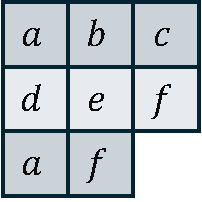
\includegraphics[width=0.2\columnwidth]{figures/target-set.pdf}} 
    \quad  \quad
	\subfloat[\label{fig:victim-set-example}]%
    {
    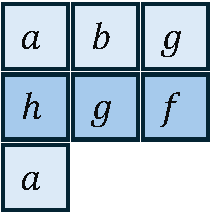
\includegraphics[width=0.204\columnwidth]{figures/victim-set.pdf}} 
    \quad  \quad
    \subfloat[\label{fig:max-recon-output} ]%
    {
    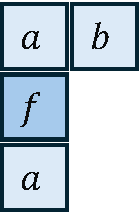
\includegraphics[width=0.149\columnwidth,trim={-0.1cm 0 -0.1cm 0},clip]{figures/max-recon.pdf}}
  \caption{
    Given a (a) target set $T$ and a (b) recovery set $Y$, we depict a (c) possible $T$-reconstruction $R_Y$. Each matched record in $Y$ corresponds to
    exactly one record in $R_Y$, and all values shared between the matched
    record and the target set $T$ appear in the corresponding record in $R_Y$.
    \label{fig:maximum-reconstruction-example}}
\end{figure}

\section{Analysis of PSU and PSU-CA}
\label{sec:psu-psuca}
\DIFaddbegin \DIFadd{In this section, we present the analysis
of PSU and PSU-CA. Since they are relatively straightfoward, we use them as a warm-up to the more involved attacks against multi-key matching in the later sections.
}

\DIFaddend While PSU and PSU-CA have received increasing attention, the information leaked by their output remains largely unstudied. \DIFdelbegin \DIFdel{It was observed by }\DIFdelend Frikken~\cite{ACNS:Frikken07}
\DIFaddbegin \DIFadd{observed }\DIFaddend that submitting an empty set in PSU fully reveals the other party's
input and proposed abort-based mitigations. Jia et al.~\cite{USENIX:JSZG24}
further analyzed PSU leakage, showing that Guo et al.'s~\cite{USENIX:GHLWJL22} PSI-CA attack extends to certain PSU variants, even under early-abort conditions, and proposed an ``enhanced'' PSU functionality that delays \DIFdelbegin \DIFdel{leakage until protocol termination}\DIFdelend \DIFaddbegin \DIFadd{protocol leakage to the end of protocol executions}\DIFaddend .

We show that such countermeasures are insufficient by \DIFdelbegin \DIFdel{introducing }\DIFdelend \DIFaddbegin \DIFadd{describing }\DIFaddend an
intersection-recovery attack \DIFdelbegin \DIFdel{on }\DIFdelend \DIFaddbegin \DIFadd{against }\DIFaddend PSU that uses only two queries and does not require the adversarial input to be empty or disjoint from the recovery set. We then prove that PSU-CA leaks at least as much information as PSI-CA by reducing
any PSI-CA attack with $q$ queries to a PSU-CA attack with $q{+}3$ queries.
%DIF < In the next section, we further show that our PSU-CA attack extends to Meta's $\calF_{\MKPM}$ functionality.


\subsection{Analysis of PSU}
\label{sec:psu-attack}
Recall that the corrupted party $\tP_1$ holds the target set $T$ and can invoke
$\calF_{\PSU}(X; Y)$ on arbitrary sets $X$ with a fixed $Y$. Its goal is to
recover $T \cap Y$. Our attack relies on the following \DIFdelbegin \DIFdel{identity,
}\begin{displaymath}
  \DIFdel{\label{eqn:PSU_basis}
  X \cap Y = (X \cup Y) \setminus (Y \setminus X) \setminus (X \setminus Y).
}\end{displaymath}%DIFAUXCMD
%DIFDELCMD <  
%DIFDELCMD < %%%
\DIFdelend \DIFaddbegin \DIFadd{observation:
}\DIFaddend 

\DIFdelbegin \DIFdel{From a $\PSU$ query, the adversary directly obtains $X \cup Y$ and can compute
$Y \setminus X = (X \cup Y) \setminus X$. The remaining challenge is to
determine $X \setminus Y$. To address this, we rely on two additional
observations, with proofs deferred to
Appendix~\ref{proof:PSU_difference_distributes}
and~\ref{proof:PSU_comp_partial_difference}, respectively.
}%DIFDELCMD < 

%DIFDELCMD < %%%
\DIFdelend \begin{proposition}\DIFdelbegin %DIFDELCMD < \label{prop:PSU_difference_distributes}
%DIFDELCMD <   %%%
\DIFdel{Let $X$ }\DIFdelend \DIFaddbegin \label{prop:PSU_recon_Y}
  \DIFadd{Let $T$ }\DIFaddend and $Y$ be sets and $X_1 \cup X_2$ be a partition of \DIFdelbegin \DIFdel{$X$}\DIFdelend \DIFaddbegin \DIFadd{$T$}\DIFaddend . It holds
  that \DIFdelbegin \DIFdel{$X \setminus Y = (X_1 \setminus Y) \cup (X_2 \setminus Y).$
}\DIFdelend \DIFaddbegin \DIFadd{$Y = (X_1 \cup Y) \cap (X_2 \cup Y)$.
}\DIFaddend \end{proposition}

\DIFdelbegin %DIFDELCMD < \begin{proposition}
%DIFDELCMD <   \label{prop:PSU_comp_partial_difference}
%DIFDELCMD <   %%%
\DIFdel{Let $X$ }\DIFdelend \DIFaddbegin \DIFadd{Proposition~\ref{prop:PSU_recon_Y} follows directly from the fact that $X_1$ }\DIFaddend and \DIFaddbegin \DIFadd{$X_2$ are disjoint. 
The recovery set }\DIFaddend $Y$ \DIFdelbegin \DIFdel{be sets and let $X_1\cup X_2$ be a partition of $X$.
Furthermore, let $Z_1 := X_1 \cup Y$ and $Z_2 := X_2 \cup Y$. Then,
  $X_1 \setminus Y = X_1 \setminus Z_2$ and
  $X_2 \setminus Y = X_2 \setminus Z_1$.
}%DIFDELCMD < \end{proposition}
%DIFDELCMD < 

%DIFDELCMD < %%%
\DIFdel{We combine Propositions~\ref{prop:PSU_difference_distributes} and
\ref{prop:PSU_comp_partial_difference} with the identity in
Eq. 
~\ref{eqn:PSU_basis} to compute $X \cap Y$ using three evaluations of
}\DIFdelend \DIFaddbegin \DIFadd{can therefore be reconstructed with only two }\DIFaddend $\PSU$ \DIFaddbegin \DIFadd{queries.
Since the adversary knows $T$, the intersection $T \cap Y$, if needed, can then be computed easily}\DIFaddend .
\DIFdelbegin \DIFdel{Moreover, one evaluation can be saved: the full union can be derived
from two partial unions, since $X \cup Y = (X_1 \cup Y) \cup (X_2 \cup Y)$.
}\DIFdelend 

We refer to this \DIFdelbegin \DIFdel{generic }\DIFdelend attack as $\PSUattack$. 
\DIFdelbegin \DIFdel{Let $X_1$ and $X_2$ be disjoint
sets forming a partition of the target set$T$, i. 
e.
}\DIFdelend \DIFaddbegin \DIFadd{Note that it requires no special inputs such as the empty set}\DIFaddend , \DIFdelbegin \DIFdel{$X_1 \cap X_2 = \emptyset$
and $X_1 \cup X_2 = T$. Then the adversarial party $\tP_1$ can recover the
intersection by querying $\calF_{\PSU}(X_1;Y)$ and $\calF_{\PSU}(X_2;Y)$. We
provide the pseudocode in Figure~\ref{fig:PSU_attack} in
Appendix~\ref{ap:psu-attack-pseudocode}.
}\DIFdelend \DIFaddbegin \DIFadd{but works with any two inputs that are disjoint from each other. 
Specific mitigation strategies that focus on prohibiting such special inputs are therefore ineffective.
%DIF > Allowing only one protocol execution per party is arguably not only unrealistic for many PSU deployment scenarios, but can also be easily circumvented via Sybil attacks.
}\DIFaddend 


\DIFdelbegin %DIFDELCMD < \begin{theorem}
%DIFDELCMD <   %%%
\DIFdel{Let $T$ be the target set and $Y$ be the recovery set. The attack
  $\PSUattack^{\calF_{PSU}(\cdot; Y)}(T)$ (Figure~\ref{fig:PSU_attack}) achieves
  intersection recovery (Def.~\ref{def:intersection-recovery}).
}%DIFDELCMD < \end{theorem}
%DIFDELCMD < \begin{proof}
%DIFDELCMD <   %%%
\DIFdel{The theorem follows from Propositions~\ref{prop:PSU_difference_distributes}
  and \ref{prop:PSU_comp_partial_difference}.
}%DIFDELCMD < \end{proof}
%DIFDELCMD < 

%DIFDELCMD < %%%
%DIF < % This is a very general attack, which only requires that $\calF_{\PSU}$ be
%DIF < % evaluated twice on disjoint sets while the recovery set $Y$ remains
%DIF < % static. These assumptions are well within the security model of proposed PSU
%DIF < % protocols.
%DIFDELCMD < 

%DIFDELCMD < %%%
\DIFdelend \subsection{PSU-CA Attack}\label{sec:PSUCA_attack}
The cardinalities of the union and intersection of two sets are \DIFdelbegin \DIFdel{closely
}\DIFdelend \DIFaddbegin \DIFadd{tightly }\DIFaddend related. We \DIFdelbegin \DIFdel{present }\DIFdelend \DIFaddbegin \DIFadd{give }\DIFaddend a generic transformation that converts any \DIFdelbegin \DIFdel{intersection
recovery }\DIFdelend \DIFaddbegin \DIFadd{intersection-recovery }\DIFaddend attack against PSI-CA (e.g.,~\cite{USENIX:GHLWJL22}) into one against PSU-CA\DIFdelbegin \DIFdel{to recover the intersection. }%DIFDELCMD < 

%DIFDELCMD < %%%
\DIFdel{Let }\DIFdelend \DIFaddbegin \DIFadd{. For sets }\DIFaddend $X$ and \DIFdelbegin \DIFdel{$Y$ be sets. Our attack relies on the following relation
,
}\begin{displaymath}\DIFdel{\label{eqn:union_intersect_cardinalities}
  |X \cap Y| = |X| + |Y| - |X \cup Y|
}\end{displaymath}%DIFAUXCMD
\DIFdelend \DIFaddbegin \DIFadd{Y, our attack uses the relation
}\[
  \DIFadd{|X \cap Y| = |X| + |Y| - |X \cup Y|.
}\]\DIFaddend 
\DIFdelbegin %DIFDELCMD < 

%DIFDELCMD < %%%
\DIFdel{This enables a translation from }\DIFdelend \DIFaddbegin \DIFadd{This equation lets us translate }\DIFaddend PSU-CA \DIFdelbegin \DIFdel{to }\DIFdelend \DIFaddbegin \DIFadd{outputs into the }\DIFaddend PSI-CA \DIFdelbegin \DIFdel{, and thus allows }\DIFdelend \DIFaddbegin \DIFadd{setting, thereby }\DIFaddend lifting any PSI-CA \DIFdelbegin \DIFdel{intersection recovery attack to the }\DIFdelend \DIFaddbegin \DIFadd{intersection-recovery attack to }\DIFaddend PSU-CA\DIFdelbegin \DIFdel{setting.
A }\DIFdelend \DIFaddbegin \DIFadd{.
The }\DIFaddend remaining challenge is that $|Y|$ is \DIFdelbegin \DIFdel{generally unknown}\DIFdelend \DIFaddbegin \DIFadd{not guaranteed to be known}\DIFaddend . We therefore \DIFdelbegin \DIFdel{present
the following method to determine }\DIFdelend \DIFaddbegin \DIFadd{show how to infer }\DIFaddend $|Y|$ \DIFdelbegin \DIFdel{with }\DIFdelend \DIFaddbegin \DIFadd{using }\DIFaddend three $\PSUCA$ evaluations\DIFdelbegin \DIFdel{that
avoids the trivial solution }\DIFdelend \DIFaddbegin \DIFadd{, while avoiding the trivial approach }\DIFaddend of querying the empty set\DIFdelbegin \DIFdel{, i.
e.,
$\calF_{\PSUCA}(\emptyset; Y)$}\DIFdelend .

\begin{proposition}\label{prop:PSUCA_comp_m}
  Let $X$ and $Y$ be two sets and let $X_1\cup X_2$ be a partition of
  $X$. Moreover, let $z:= |X \cup Y|$, $z_1 := |X_1 \cup Y|$ and
  $z_2 := |X_2 \cup Y|$. Then, we have $|Y| = z_2 - (z - z_1)$.
\end{proposition}

The proof is provided in Appendix~\ref{proof:PSUCA_comp_m}. Thus, with three
additional $\calF_{\PSUCA}$ evaluations at the start of the attack, the
adversary can simulate the $\calF_{\PSICA}$ functionality. In particular, for
any PSI-CA attack, the adversary can replace each query
$z\gets \calF_{\PSICA}(X;Y)$ with $z'\gets \calF_{\PSUCA}(X;Y)$ and then compute
$z$ as $|X|+|Y|-z'$.

We state our result in the following theorem:
\begin{theorem}\label{thm:PSICA-to-PSUCA}
  For every adversary $\adv$ such that
  $\adv^{\calF_{\PSICA}(\cdot; Y)}(T) = T \cap Y$ which makes $q$ $\PSICA$
  queries, there is an efficient adversary $\bdv$ with access to
  $\calF_{\PSUCA}(\cdot; Y)$ which recovers $T \cap Y$ and makes $q + 3$
  $\PSUCA$ queries.
\end{theorem}

The proof is given in Appendix~\ref{proof:PSICA-to-PSUCA}. In
Appendix~\ref{attack:PSUCA}, we describe and analyze
$\PSUCAattack$---an attack that uses the transformation described above to turn
the PSI-CA attack from Guo et al.\DIFdelbegin \DIFdel{\mbox{%DIFAUXCMD
\cite{USENIX:GHLWJL22} }\hskip0pt%DIFAUXCMD
(See
Appendix~\ref{ap:guo_attack} for an overview) }\DIFdelend \DIFaddbegin \DIFadd{~\mbox{%DIFAUXCMD
\cite{USENIX:GHLWJL22} }\hskip0pt%DIFAUXCMD
}\DIFaddend to one against PSU-CA.
\section{\DIFdelbegin \DIFdel{Matachable }\DIFdelend \DIFaddbegin \DIFadd{Matchable }\DIFaddend Record Recovery with $\calF_{\MKPM}$}\label{sec:PSUCA_to_matching}
In this section, we show how the $\PSUCAattack{}$ attack can be applied to $\calF_{\MKPM}$ with some additional assumptions to achieve \emph{matchable record recovery}
(Definition~\ref{def:matchable_records_recovery}). In
Appendix~\ref{sec:psuca-privateID-attack} we explain how the attack can
be applied to the single key private matching functionality $\calF_{\SKPM}$ realized by PrivateID~\cite{PMC}.

\DIFdelbegin \DIFdel{The adversary is }\DIFdelend \DIFaddbegin \subsection{\DIFadd{A Primer on Guo et al.'s PSI-CA Attack}}
\DIFadd{Before describing our attack, we briefly review Guo et al.’s~\mbox{%DIFAUXCMD
\cite{USENIX:GHLWJL22} }\hskip0pt%DIFAUXCMD
intersection-recovery attack against the PSI-CA functionality,which outputs the intersection cardinality \(|X \cap Y|\). 
}

\DIFadd{In Guo et al.’s attack, the adversary has a target set $X$ and can query the PSI-CA functionality $\calF_{\PSICA}(\cdot ;Y)$ on adaptively chosen sets $X' \subseteq X$, where $Y$ is a fixed recovery set. The goal is to recover $X \cap Y$. The key observation is that some PSI-CA outputs immediately reveal membership information: (1) if $|X' \cap Y| = 0$, then no element of $X'$ lies in $Y$ and (2) if $|X' \cap Y| = |X'|$, then every element of $X'$ lies in $Y$.
}

\DIFadd{To exploit this, the adversary builds a balanced binary search tree over $X$, where each node contains a subset of $X$ and its children form a partition of that subset. The adversary traverses the tree and queries PSI-CA on selected nodes until it finds subsets whose membership can be fully determined by the two termination cases above. Since the children partition their parent, the adversary can infer one child’s intersection cardinality from the parent and sibling values, reducing the number of queries needed: if $X_1 \cup X_2$ is a disjoint partition of $X$, we have $|X_2 \cap Y| = |X \cap Y| - |X_1\cap Y|$. Repeating this process recursively allows the adversary to label elements as either in $X\cap Y$ or in $X \setminus Y$, thereby recovering the intersection.
}

\DIFadd{We give a pictorial example of the attack in Figure~\ref{fig:guo_basline_tree} and a more detailed description of the attack in Appendix~\ref{ap:guo_attack}.
}

\begin{figure}
  \centering
  {	\colorlet{positive}{LimeGreen}
    \colorlet{negative}{BrickRed}
    \newcommand{\pos}[1]{\raisebox{.9pt}{#1}}
    \newcommand{\fullcirc}{\position{\tikz{\draw[line width=.5pt, color=black, fill=black] circle(1.1pt);}}}
    \newcommand{\ocirc}{\position{\tikz[]{\draw[line width=.5pt, color=black, fill=none] circle(1.1pt);}}}

    \begin{tikzpicture}
      [
      level 1/.style = {sibling distance = 4cm},
      level 2/.style = {sibling distance = 2cm},
      level 3/.style = {sibling distance = 1.5cm}
      ]
      {	\tiny
        \node {\fullcirc\;$X = \{1, 2, 3, 4, 5, 6\}$}[level distance =.8cm]
        child {node {\fullcirc\;$X_{1,1} = \{1, 2, 3\}$}
          child {node {\fullcirc\;\color{positive}$X_{2,1} = \{1, 2\}$} {
              child {node {\color{positive}$X_{3,1} = \{1\}$}}
              child {node {\color{positive}$X_{3,2} = \{2\}$}}
            }}
          child {node {\ocirc\;\color{negative}$X_{2,2} = \{3\}$}}}
        child {node {\ocirc\;\color{negative}$X_{1,2} = \{4, 5, 6\}$}
          child {node {\color{negative}$X_{2,3} = \{4, 5\}$} {
              child {node {\color{negative}$X_{3,3} = \{4\}$}}
              child {node {\color{negative}$X_{3,4} = \{5\}$}}
            }}
          child {node {\color{negative}$X_{2,4} = \{6\}$}}};}
    \end{tikzpicture}
    \caption{
      \DIFaddFL{The binary search tree for the target set $X=\{1,2,3,4,5,6\}$ in the intersection-recovery attack of~\mbox{%DIFAUXCMD
\cite{USENIX:GHLWJL22}}\hskip0pt%DIFAUXCMD
, shown for recovery set \(Y=\{1,2\}\). Nodes marked with $\circ$ are queried via PSI-CA, while nodes marked with $\bullet$ have their intersection cardinality inferred from their parent and sibling. Depth first search terminates early at \(X_{2,1}\) and \(X_{1,2}\). Inferred membership is shown in }{\color{positive} \DIFaddFL{green}} \DIFaddFL{for $X\cap Y$ and }{\color{negative} \DIFaddFL{red}} \DIFaddFL{for $X\setminus Y$.}}
    \label{fig:guo_basline_tree}
  }
\end{figure}

\subsection{\DIFadd{From Union to UID Cardinalities}}
\DIFadd{In the context of MKPM,
the adversary is }\DIFaddend given a target set of records $T \subseteq \Ispace{}^n$, and
can evaluate $\calF_{\MKPM}(X; Y)$ for arbitrarily many inputs $X$. Its goal is
to determine the set of matchable records, $T \sqcap Y$. The functionality
$\mathcal F_{\MKPM}$ outputs the set universal identifiers, $\UID$, to both
parties. Rather than assigning a common UID to two identical records, it applies
a matching logic (see Figure~\ref{fig:match_logic}) which assigns a common UID
to each pair of matched records, and a distinct UID to every unmatched record in
$T$ and $Y$. Thus, using $|\UID|$ as the cardinality for carrying out
$\PSUCAattack{}$ appears to be a natural approach for identifying matching
records in $T$.

The $\PSUCAattack{}$ attack (Section~\ref{sec:PSUCA_attack}) relies
on the fact that $|X \cup Y| = |X_1 \cup Y| + |X_2 \cup Y| - |Y|$
\DIFdelbegin \DIFdel{(Eq.~\ref{eqn:union_intersect_cardinalities}), }\DIFdelend %DIF > (Prop.~\ref{prop:PSUCA_comp_m}), 
where $X$ and $Y$ are arbitrary
sets and $X_1\cup X_2$ form a partition of $X$. We now translate this to the
multi-key setting. Let $\UID$, $\UID_1$, and $\UID_2$ be the UIDs output when
evaluating $\calF_{\MKPM}(X; Y)$ and $\calF_{\MKPM}(X_i; Y)$ for
$i \in \{1, 2\}$ respectively. For the attack to apply, we require the following
relation to hold:
\begin{equation}
  \label{eqn:MKPM_PSUCA_condition}
  |\UID| = |\UID_1| + |\UID_2| - |Y|.
\end{equation}

Unfortunately, this condition does not hold for general inputs. The reason is
that the MKPM functionality shuffles the inputs before applying the matching
logic. Consequently, the matching procedure introduces randomness, leading to
inconsistent record matches across different protocol runs, even with the same
input sets. Thus, different evaluations of $\calF_\MKPM$ on identical inputs can
yield $\UID$ sets with varying cardinalities.

We give an example of such a matching in
Figure~\ref{fig:MPMK_PSUCA_counterexample}.

To rule out such cases, we impose a restriction on the input sets that, if
satisfied, ensures that Eq.~\ref{eqn:MKPM_PSUCA_condition} holds, thus allowing
us to carry out the attack. Luckily, one-to-many relations do not violate
Eq.~\ref{eqn:MKPM_PSUCA_condition}. It therefore suffices to exclude many-to-one
relations.

\begin{definition}\label{def:isolated_set}
  Let $X, Y$ be sets of records.
  We say $X$ is \textbf{$Y$-isolated}, 
  if for all $\by\in Y$ we have 
  $$|\{\bx \in X \setdsc \exists i, j \text{ s.t. } \bx[i] = \by[j]\}|
  \leq 1.$$
\end{definition}

This constraint may exclude certain scenarios. For example, if the sets contain
IP addresses, many-to-one relationships are likely to occur since multiple users
in the same local network share an IP address. However, the adversary's input
may be $Y$-isolated in scenarios where the adversary targets a specific range of
identifiers, such as all phone numbers with a specific area code or all email
addresses from a particular domain.

\begin{theorem}\label{thm:psu-mkpm:correctness}
  Let $T,V\subseteq \Ispace{}^n$ be sets of records. If $T$ is $Y$-isolated,
  then $\PSUCAattack^{\calF_{\MKPM}(\cdot; Y)}(T)$ recovers $T \sqcap Y$.
\end{theorem}

The proof can be found in Appendix~\ref{sec:psu-mkpm:correctness}.

\heading{Time and Query Complexity.} The $\PSUCAattack{}$ can be applied
directly to the output of $\calF_{\MKPM}$, as long as the adversary's input sets
satisfy Definition~\ref{def:isolated_set}. The attack thus has the same worst-case time complexity and maximum number of protocol invocations as when
applied to $\calF_{\PSUCA}$. Specifically, it requires $\bigO{n\log n}$ time and
at most $n + 1$ protocol invocations (although typically fewer queries are
needed due to the probability of early termination).

\begin{figure}
  \centering
  {\def\linecorr{-.4pt} % Reduced correction for tighter placement
	\def\rowspace{1cm} % Adjust row space
	\def\colspace{2.5cm} % Widen the figures
	\def\setspace{0.2cm} % Reduce space between figures
	\def\setvertspace{.5cm} % Adjust vertical space between figure rows
	\def\minwidthid{0.6cm} % Slightly smaller blocks
	\def\blockminheight{1.3em} % Slightly smaller blocks
	\begin{tikzpicture}
		[block/.style={draw,minimum width=#1, minimum height=\blockminheight,font={\small}},
		block/.default=10em,high/.style={},auto,
		node distance=0, % Initially 0 to control spacing
		>=Stealth]

		% Top Figure
		% Nodes
		\node[block=\minwidthid,fill=trow-dark] (alice1) {$v_1$};
		\node[block=\minwidthid,fill=trow-dark, right=\linecorr of alice1] (alice2) {$v_2$};

		\node[block=\minwidthid,fill=trow-light, below=\linecorr of alice1] (bob1) {$v_3$};
		\node[block=\minwidthid,fill=trow-light, right=\linecorr of bob1] (bob2) {$v_4$};

		%\coordinate (mid) at ($(alice2)!0.5!(bob2)$);

		\node[block=\minwidthid,fill=trow-dark, right=\colspace of alice2.south east] (vic1) {$v_3$};
		\node[block=\minwidthid,fill=trow-dark, right=\linecorr of vic1] (vic2) {$v_2$};


		% Connections
		\draw[dashed] (alice2) to (vic1);
		\draw (bob2) to (vic1);

		% Labels and descriptions
		\coordinate (center1) at ($(alice2.east)!0.5!(vic1.west)$);

		\node[left=.3cm of alice1.south west] (Tlabel) {$T$};
		\node[right=.3cm of vic2.east] (Vlabel1) {$Y$};
		\node[below=.5cm of center1] (UIDlabel) {$|\UID| = 2$};

		% Bottom Figure
		% Adjust vertical placement by node distance and below distance
		\coordinate (bottom_start) at ($(bob1.south) + (0,-\setspace)$);

		\node[block=\minwidthid,fill=trow-dark, below=\setvertspace of bottom_start] (alicesub1) {$v_1$};
		\node[block=\minwidthid,fill=trow-dark, right=\linecorr of alicesub1] (alicesub2) {$v_2$};
		\node[block=\minwidthid,fill=trow-dark, right=\colspace of alicesub2] (vicsub1) {$v_3$};
		\node[block=\minwidthid,fill=trow-dark, right=\linecorr of vicsub1] (vicsub2) {$v_2$};

		\node[block=\minwidthid,fill=trow-dark, below=\setvertspace of alicesub1] (bobsub1) {$v_3$};
		\node[block=\minwidthid,fill=trow-dark, right=\linecorr of bobsub1] (bobsub2) {$v_4$};
		\node[block=\minwidthid,fill=trow-dark, right=\colspace of bobsub2] (vicsub3) {$v_3$};
		\node[block=\minwidthid,fill=trow-dark, right=\linecorr of vicsub3] (vicsub4) {$v_2$};

		% Connections
		\draw (alicesub2) to (vicsub1);
		\draw (bobsub2) to (vicsub3);

		% Labels and descriptions
		\coordinate (center2) at ($(alicesub2.east)!0.5!(vicsub1.west)$);
		\coordinate (center3) at ($(bobsub2.east)!0.5!(vicsub3.west)$);

		\node [left=.3cm of alicesub1.west] (Tlabel2) {$T_1$};
		\node [right=.3cm of vicsub2.east] (Vlabel2) {$Y$};
		\node [below=0cm of center2] (UIDlabel1) {$|\UID_1| = 1$};

		\node [left=.3cm of bobsub1.west] (Tlabel3) {$T_2$};
		\node [right=.3cm of vicsub4.east] (Vlabel3) {$Y$};
		\node [below=0cm of center3] (UIDlabel2) {$|\UID_2| = 1$};
\end{tikzpicture}}
  \caption{An example that $\PSUCAattack{}$ attack cannot be applied to the output of $\calF_{\MKPM}(T;Y)$. Lines between records indicate potential matches based on matching values. Solid lines denote the matched records
  chosen by the matching logic. We see that
    $|\UID| \neq |\UID_1| + |\UID_2| - |Y|$ and, as such, $T$ is not
    $Y$-isolated.}
  \label{fig:MPMK_PSUCA_counterexample}
\end{figure}

\section{Value Intersection Recovery with $\calF_{\LMKPM}$}\label{sec:st-mkpm-attack}

We now leverage the additional leakage that $\calF_{\LMKPM}$ outputs to $\tP_1$ to mount stronger attacks. We adapt Guo et al.'s search tree approach~\cite{USENIX:GHLWJL22}, designed for $\calF_{\PSICA}$, to recover the shared values and achieve \emph{value intersection recovery} (Def.~\ref{def:VIR_goal}). 
%In the full version, we additionally show how to recover the multiplicities of each value.

For this attack, we restrict the adversary to using only subsets of its target set $T$ as input: it may submit any $T' \subseteq T$ but cannot append, split, or rearrange the values within records (this contrasts with Section~\ref{sec:lmkpm-attacks}, where the adversary can modify record contents by appending or reordering values). 
We assume all records in $T$ have equal length $\ell_{\rec} \in \NN$. 
The goal is to compute the intersection of values which we denote as $\posSet := \Ispace[T] \cap \Ispace[Y]$. Throughout the attack, we also construct a second set, $\negSet := \Ispace[T] \setminus \Ispace[Y]$, of values in $T$ that are not in $Y$. 

% Recall that the output of $\calF_{\LMKPM}(X;Y)$ to party $\tP_1$ is
% \[
% (\UID, \MX, \leak^1) = (\UID, \MX, (\hXone, \hYone)),
% \]
% where $\UID$ denotes the set of all assigned UIDs, $\MX$ is the local mapping from UIDs to records in $X$, and $(\hXone, \hYone)$ are the hidden, shuffled records of $X$ and $Y$, respectively. 

%DIF >  \subsection{Leveraging the Search Tree Approach}
\DIFaddbegin 


\DIFaddend Our adapted attack starts by building a binary search tree $\calT$ over $T$ similar to \DIFdelbegin \DIFdel{the original }\DIFdelend \DIFaddbegin \DIFadd{Guo et al.'s }\DIFaddend attack~\cite{USENIX:GHLWJL22}. The root node corresponds to the entire target set $T$. Each node $v$ is labeled with a subset $v.\treeSet \subseteq T$. Its children $v_L \gets v.\treeLeftChild$ and $v_R \gets v.\treeRightChild$ form a disjoint partition of the parent:
$v_L.\treeSet \cup v_R.\treeSet = v.\treeSet$ and $v_L.\treeSet \cap v_R.\treeSet = \emptyset$.
We use a fixed, deterministic rule to compute the partition (e.g., by index into equal halves) and recurse until leaves are single records. 


Starting at the root, the adversary traverses $\calT$ in DFS order, selecting a node at each step and querying $\calF_{\LMKPM}(\cdot; Y)$ on that node’s associated subset of records. Let $X \gets v.\treeSet$ for a non-leaf node $v$, and $X_1 \gets v_L.\treeSet$, $X_2 \gets v_R.\treeSet$ be its children. In Guo et al.'s PSI-CA attack, querying a parent $X$ and one child $X_1$ suffices to infer the sibling’s output: from $|X \cap Y|$ and $|X_1 \cap Y|$ one immediately obtains $|X_2 \cap Y|$ without a third query.

Under $\calF_{\LMKPM}$, this sibling inference is not possible: each query
generates UIDs with fresh randomness, so given $(\leakX{}, \leakY)$ and
$(\leakX{1}, \leakY)$, one cannot derive $(\leakX{2}, \leakY)$. Instead of
inferring the sibling’s full leakage, we switch to a metric for which the
sibling’s value \emph{can} be inferred without an additional query---namely, the
number of matched values \emph{per column} in $\leakX{}$ and $\leakX{1}$---and
use this to guide the DFS traversal. Formally, this metric is defined as:
\begin{equation*}
  \text{ColCA}(\leakX{}, \leakY) :=
  \left(\sum_{\bt\in\leakX{}}\mathbbm{1}\{\bt[i] \in
    \Ispace[\leakY]\}\right)_{i\in[\ell_{\rec}]}.
\end{equation*}

% \begin{align*}
%     \text{Col}&\text{CA}(\leakX{}, \leakY) \\
% 	&:= \left(\sum_{\bt\in\leakX{}}\mathbbm{1}\{\bt[1] \in
% 	\Ispace[\leakY]\}, \dots,
% 	\sum_{\bt\in\leakX{}}\mathbbm{1}\{\bt[\ell_{\rec}] \in
%  \Ispace[\leakY]\}\right).
% \end{align*}

We make the following important observations about \colCA.
\begin{proposition}
	\label{prop:mkpsi_equiv}
	For any two sets of records $X$ and $Y$, we have
	\begin{equation*}
		\colCA(\leakX{}, \leakY) = \colCA(X, Y).
	\end{equation*}
\end{proposition}
In words, because the hiding function used is deterministic, the leakage preserves the per-column counts of matching values between the plaintext inputs $X$ and $Y$.

\begin{proposition}
	\label{prop:mkpsi_inference}
	Let $X$ and $Y$ be sets of records, and let $X_1 \cup X_2$ be a partition of $X$. Then we have
\begin{equation*}
		\colCA(\leakX{}, \leakY)
		= \colCA(\leakX{1}, \leakY) + \colCA(\leakX{2}, \leakY)\footnote{We use standard vector operations; addition and subtraction are applied element-wise.}.
	\end{equation*}
\end{proposition}

Proofs are given in Appendix~\ref{proof:mkpsi_equiv} and~\ref{proof:mkpsi_inference}, respectively.

From Prop.~\ref{prop:mkpsi_inference} we obtain $\colCA(\leakX{2}, \leakY)
  = \colCA(\leakX{}, \leakY) - \colCA(\leakX{1}, \leakY).$
Here, $\leakX{2}$ denotes the (hypothetical) leakage from a protocol run on $X_2$, which is never actually executed. This suffices, since we only need $\colCA(\leakX{2}, \leakY)$, and this vector can be inferred without knowing $\leakX{2}$ explicitly.

For a leaf node containing a single record, i.e., $X = \{\bx\}$, the vector $\colCA(\leakX{},\leakY)$ is binary: its $i$-th entry is $1$ if and only if the $i$-th value of $\bx$ appears in $Y$, and $0$ otherwise.
More generally, consider any node with record set $X$. Suppose that after querying this node we obtain
\[
    \bc=\colCA(\leakX{}, \leakY) \in \{0, |X|\}^{\ell_{\rec}}.
\]
By Prop.~\ref{prop:mkpsi_equiv}, this equals $\colCA(X,Y)$, so the $i$-th entry counts how many records in $X$ have their $i$-th value in $\Ispace[Y]$. If the $i$-th entry is $|X|$, then \emph{every} record in $X$ has its $i$-th value in $Y$; if it is $0$, then \emph{no} record in $X$ has its $i$-th value in $Y$. Thus, for such a node, each column is either entirely positive (all values occur in $Y$) or entirely negative (no value occurs in $Y$).
Thus for each $i\in[0,\dots,\ell_{\rec}-1]$ if $\bc[i]=|X|$ we add $\{\bx[i]: \bx\in X\}$ to $\posSet$, and otherwise we add it to $\negSet$. Once we have processed all the nodes in this way, $\posSet$ must include all values in $\Ispace[T]\cap\Ispace[Y]$.

% For a leaf node storing a single record, i.e., $X = \{\bx\}$, the vector $\colCA(\leakX{},\leakY)$ is binary: its $i$-th entry is $1$ if and only if the $i$-th value of $\bx$ appears in $Y$, and $0$ otherwise. More generally, once a node is queried and the resulting sum entry in the vector is the number of records in that set,

% $\colCA(\leakX{}, \leakY) \in \{0, |X|\}^{\ell_{\rec}}$ for some $X$, Prop.~\ref{prop:mkpsi_equiv} implies that, for each column, either all or none of the values in that column of $X$ occur in $Y$, depending on whether the corresponding entry equals $|X|$ or $0$.


The remaining component of our adapted attack is a heuristic that (i) decides which child to follow during DFS traversal and (ii) provides the priority for enqueuing the other child. For any set $X$, this heuristic must be computable from $X$ and $\colCA(\leakX{}, \leakY)$ alone, since this is all we know about the (hypothetical) leakage for that node. For $\bc = \colCA(\leakX{}, \leakY)$, we define
\begin{equation}
      p_{MK}^+(\bc, X) := \frac{\sum_{x \in \bc} x}{\ell_{\rec} |X|}.
\end{equation}
As in the original PSI-CA attack~\cite{USENIX:GHLWJL22}, our heuristic prioritizes the child node whose subsets contain more matched values, which increases the fraction of the intersection that can be recovered when the adversary is limited to a bounded number of protocol invocations.
We additionally propose two further heuristics in~\ref{ap:IRR:heuristics} and evaluate our three heuristics in Appendix~\ref{ap:evaluation}. 

The pseudocode of \mkpsiattack{} is given in Figure~\ref{fig:MKPSIattack} (Appendix~\ref{ap:VIR}).
%The attack is similar to the original PSI-CA attack, with the difference that we maintain two sets $\posSet$ and $\negSet$ to keep track of the inferred positive and negative membership information.

\begin{theorem}\label{thm:VIR-attack-correctness}
  $\mkpsiattack^{\calF_{\LMKPM}(\cdot;Y)}(T)$ (Figure~\ref{fig:MKPSIattack})
  achieves value intersection recovery (Def.~\ref{def:VIR_goal}).
\end{theorem}
The proof can be found in Appendix~\ref{proof:VIR-attack-correctness}.

\heading{Time and Query Complexity.}  Let $n = |T|$, $m = |Y|$, and let
$\ell_{\rec}$ be the maximum record length in $T$ and $Y$. Assume $n$ is a power
of two and that priority-queue operations \push{} and \pop{} take amortized time
\bigO{\log n}. Since $n$ nodes are pushed and popped in total, this contributes
\bigO{n \log n} time.  For inputs $X$ of size $a$ and $Y$ of size $b$,
$\colCA(X,Y)$ can be computed in expected time \bigO{\ell_{\rec}(a+b)}. It is
called once at the root and for half the nodes at each depth, yielding an
expected total cost of $\bigO{\ell_{\rec} n(\log n + m)}$. The heuristic
$p_{MK}^+$ adds only lower-order terms, so the overall expected runtime is
$\bigO{\ell_{\rec} n(\log n + m)}$.

Like the original PSI-CA attack, \mkpsiattack{} requires at most $n$ protocol
invocations, though this bound is loose due to early termination of DFS
traversals (see Section~\ref{sec:evaluation} for an empirical evaluation).  Even
when the number of protocol invocations is restricted, partial intersection
recovery remains feasible (see Appendix~\ref{ap:evaluation}).
\section{$T$-Reconstruction with $\calF_{\LMKPM}$}\label{sec:lmkpm-attacks}
In this section, we describe three powerful attacks that exploit the ``leaky''
functionality $\calF_{\LMKPM}$. Buddhavarapu et al.~\cite{MKPMC} acknowledge
this leakage but deem it acceptable as an aggregate metric that would only raise
concerns across multiple executions. In contrast, we present three attacks that
achieve \emph{$T$-reconstruction} (Definition~\ref{def:max_recons}) with a
single protocol invocation.

We first present a baseline attack that is highly efficient but relies on a
strong assumption on the protocol inputs. We then describe two additional
attacks that progressively relax these assumptions.

% All three attacks preprocess the target set $T$ so that the resulting records are uniquely identifiable from the protocol output in a single invocation. This allows the adversary to map hidden identifiers revealed by the leakage back to their plaintext values. 

\subsection{The Baseline Attack}
\label{sec:baseline-attack}
Recall that while the records in the adversary's input $X$ are hidden and shuffled, the order of values \emph{within} each record is preserved.
We first observe that matching records between $X$ and the leakage $\hXone$ is trivial when $X$
contains one record. Exploiting this, we present \baselineattack{}, which
flattens the target set $T$ into an input $X$ consisting of a single record \DIFaddbegin \DIFadd{$\br$ }\DIFaddend that
contains all values in $\Ispace[T]$.

The baseline attack constructs a dictionary $\Dict$ that maps hidden values appearing in the leakage $\hXone = \{\hbx\}$ back to their original plaintext values in the input $X = \{\bx\}$. Specifically, for all $j = 0, \dots, |\hbx|$, the adversary sets
\[
    \Dict : \hbx[j] \mapsto \bx[j].
\]
It then uses $\Dict$ to recover plaintext values in the recovery set
$\hYone$. It initializes an empty multiset $R_Y$, and for each hidden record
$\hby_i \in \hYone$ it initializes an empty record $\bs_i$. For all
$j = 0, \dots, |\hby_i|$, it checks whether $\hby_i[j] \in \Dict$; if so, it
appends $\Dict[\hby_i[j]]$ to $\bs_i$. Finally, it adds $\bs_i$ to $R_Y$. In
this way, the adversary recovers the plaintexts of all values in $Y$ that are in
common with those in $T$. This procedure yields a $T$-reconstruction $R_Y$ of
$Y$.

\DIFdelbegin \DIFdel{We omit a full proof of correctness. }\DIFdelend \DIFaddbegin \DIFadd{The pseudocode of \baselineattack{} is shown in Figure~\ref{fig:toy_attack} (left).  
We also define an algorithm $\dictInfer$ that takes a set of hidden records $\leak^1_Y$ and a dictionary $D: G \to \Ispace{}$ mapping hidden to plaintext values, and replaces the values in the records of $\leak^1_Y$ with the corresponding entries in $D$. Identifiers that do not occur in $D$ are not replaced. This algorithm is used as a subroutine in all attacks in this section and is given in Figure~\ref{fig:toy_attack} (right).
}


\DIFaddend Correctness of the attack directly follows
from the fact that all values in the flattened target record are uniquely
identifiable in a single invocation of $\calF_{\LMKPM}$. 

\heading{Time and Query Complexity.}
Let $\ell_{\rec}$ denote the maximum record length in $T$ and $Y$. Let $n = |T|$ and $m = |Y|$.
The attack has an asymptotic time complexity of
$\bigO{\ell_{\rec}(n + m)}$.
%The membership check can be reduced to constant time by maintaining an auxiliary set of already added identifiers, as set membership can be tested in constant time.
The attack requires only one query and therefore establishes a tight lower bound on the number of queries needed to achieve TR (Definition~\ref{def:max_recons}).

%DIF <  \begin{figure*}
%DIF <  	\input{pseudocode/recenum-code.tex}
%DIF <  	\caption{Record enumeration attack $\recenumattack$ with oracle access to the extended MK-PrivateID functionality $\calF_{LMKPM}(\cdot; Y)$. 
%DIF <  	Note that $Y$ is part of the oracle and not known to the adversary.}\label{fig:rec_enum_attack}\label{fig:idx_to_seq}\label{fig:seq_to_idx}\label{fig:dict_infer}
%DIF <  \end{figure*}
\DIFaddbegin \begin{figure}
	\centering
	\begin{pchstack}[boxed, center]
		\pchspace
		\procedure[linenumbering]{$\baselineattack^{\calF_{\LMKPM}(\cdot, Y)}(T)$}{%
            \rule{0pt}{2em}%
			\br \gets () \label{lin:baseline_r_start}\\
			\pcfor \bt \in T \pcdo \\
			    \t	\pcfor i = 1, \dots, |\bt| \pcdo \label{lin:toy_attack_membership_check}\\
			        \t	\t	\pcif \bt[i] \not\in \br \pcthen \\
			            \t	\t	\t	\br \gets \br \| \bt[i] \label{lin:baseline_r_end}\\
			X \gets \{\br\} \label{lin:toy_attack_def_T_prime} \\
			(\UID, \MC, (\leak_X^1, \leakY))\pcskipln \\
            \t\t \sample \calF_{\LMKPM}(X, Y) \label{lin:baseline_eval}\\
			\{\hat{\br}\} \gets \leak^1_X \\
			\text{Initialize dictionary $D\gets\emptyset$} \\
			\pcfor i \in [0, |\hat{\br}|-1] \pcdo \label{lin:baseline_D_start}\\
			\t	D[\hat{\br}[i]] \gets r[i] \label{lin:baseline_D_end}\\
			R_Y \gets \dictInfer(\leak^1, D) \\
			\pcreturn R_Y
		}
		\DIFaddFL{\hspace{2mm}
		}\procedure[linenumbering]{$\dictInfer(\leak^1_Y, D)$}{
        \rule{0pt}{2em}%
		\text{Initialize $R\gets\emptyset$} \\
		\pcfor \hby \in \leak^1_Y \pcdo \\
		\t	\br \gets () \\
		\t	\pcfor i \in [0, |\hby|-1] \pcdo \\
		\t	\t	\pcif \hby[i] \in D \pcthen \label{lin:substitute_membership_check} \\
		\t	\t	\t	\br \gets \br \| D\left[\hby[i]\right] \label{lin:substitute_add_id} \\
		\t	R \gets R \cup \{\br\} \label{lin:substitute_add_record}\\
		\pcreturn R
	}
	\end{pchstack}
	\caption{\DIFaddFL{Baseline attack with oracle access to the MKPM functionality with leakage $\calF_{\LMKPM}(\cdot, Y)$. 
	$Y$ is part of the oracle and is unknown to the adversary.
	}} \label{fig:toy_attack} \label{fig:dict_infer}
\end{figure}
\DIFaddend 


\begin{figure}[t]
    \centering
    \def\rowspace{-.4pt}
    \def\minwidthemail{2.5cm}
    \def\minwidthphone{2.5cm}
    \def\minwidthid{.6cm}
    \def\linecorr{-.4pt}
    \def\blockminheight{1.5em}
    \definecolor{added-id}{HTML}{15b01a}
    \definecolor{matched-light}{HTML}{DCEDC8}
    \definecolor{matched-dark}{HTML}{C4E1A3}
    \definecolor{tiebreaker}{HTML}{A3CEE1}
    \definecolor{highlight-blue}{HTML}{4A90E2} 
    % Subfigures
    \subfloat[Target set $T$ (boxed in blue) and input set $X$ (the entire table).\label{subfig:recenum_example_plain}]{
        %\resizebox{1\columnwidth}{!}{%
        \begin{tikzpicture}
  [block/.style={draw,minimum width=#1, minimum height=\blockminheight,font={\small}},
	block/.default=10em,high/.style={},auto,
	node distance=0, 
	>=Stealth]

% Nodes
\node[block=\minwidthid, draw=none ] (alice_idx) {$\bx_0:$};
\node[block=\minwidthid,fill=matched-light, right=\linecorr of alice_idx] (alice1) {$v_0$};
\node[block=\minwidthid,fill=matched-light, right=\linecorr of alice1] (alice2) {$v_0$};
\node[block=\minwidthemail,fill=trow-dark, right=\linecorr of alice2] (alice3) {alice@mail.com};
\node[block=\minwidthphone,fill=trow-dark, right=\linecorr of alice3] (alice4) {+41 98 765 43 21};

\node[block=\minwidthid, draw=none, below=\rowspace of alice_idx] (bob_idx) {$\bx_1:$};
\node[block=\minwidthid,fill=trow-light, right=\linecorr of bob_idx] (bob1) {$v_0$};
\node[block=\minwidthid,fill=trow-light, right=\linecorr of bob1] (bob2) {$v_1$};
\node[block=\minwidthemail,fill=trow-light, right=\linecorr of bob2] (bob3) {bob@mail.com};
\node[block=\minwidthphone,fill=trow-light, right=\linecorr of bob3] (bob4) {+41 12 345 67 89};

\node[block=\minwidthid,below=\rowspace of bob_idx, draw=none ] (eve_idx) {$\bx_2:$};
\node[block=\minwidthid,fill=trow-dark, right=\linecorr of eve_idx] (eve1) {$v_1$};
\node[block=\minwidthid,fill=trow-dark, right=\linecorr of eve1] (eve2) {$v_0$};
\node[block=\minwidthemail,fill=trow-dark, right=\linecorr of eve2] (eve3) {eve@mail.com};
\node[block=\minwidthphone,fill=trow-dark, right=\linecorr of eve3] (eve4) {+41 45 678 91 23};

\node[block=\minwidthid,below=\rowspace of eve_idx, draw=none ] (gus_idx) {$\bx_3:$};
\node[block=\minwidthid,fill=trow-light, right=\linecorr of gus_idx] (gus1) {$v_1$};
\node[block=\minwidthid,fill=tiebreaker, right=\linecorr of gus1] (gus2) {$v_2$};
\node[block=\minwidthemail,fill=trow-light, right=\linecorr of gus2] (gus3) {gus@mail.com};
\node[block=\minwidthphone,fill=trow-light, right=\linecorr of gus3] (gus4) {+41 56 789 12 34};

% Rectangles
\draw[draw=added-id, line width=.7pt] (alice1.north west) rectangle (gus2.south east); % green
\draw[draw=highlight-blue, line width=.7pt] (alice3.north west) rectangle (gus4.south east); % blue

\end{tikzpicture}

        %}
    }
    \quad
    \subfloat[The hidden, shuffled leakage $\hXone$.\label{subfig:recenum_example_leakage}]{
        %\resizebox{0.48\columnwidth}{!}{%
        \hspace{0.5cm}

\begin{tikzpicture}
	[block/.style={draw,minimum width=#1, minimum height=\blockminheight,font={\small}},
	block/.default=10em,high/.style={},auto,
	node distance=0, 
	>=Stealth]
	% Nodes
	\node[block=\minwidthid, draw=none] (eve_idx) {$\bx_2:$};
	\node[block=\minwidthid,fill=trow-dark, right=\linecorr of eve_idx](eve1) {$e_0$};
	\node[block=\minwidthid,fill=trow-dark, right=\linecorr of eve1] (eve2) {$e_1$};
	\node[block=\minwidthid,fill=trow-dark, right=\linecorr of eve2] (eve3) {$e_2$};
	\node[block=\minwidthid,fill=trow-dark, right=\linecorr of eve3] (eve4) {$e_3$};

	\node[block=\minwidthid,below=\rowspace of eve_idx, draw=none ] (bob_idx) {$\bx_1:$};
	\node[block=\minwidthid,fill=trow-light, right=\linecorr of bob_idx] (bob1) {$e_1$};
	\node[block=\minwidthid,fill=trow-light, right=\linecorr of bob1] (bob2) {$e_0$};
	\node[block=\minwidthid,fill=trow-light, right=\linecorr of bob2] (bob3) {$e_4$};
	\node[block=\minwidthid,fill=trow-light, right=\linecorr of bob3] (bob4) {$e_5$};

	\node[block=\minwidthid,below=\rowspace of bob_idx, draw=none ] (gus_idx) {$\bx_3:$};
	\node[block=\minwidthid,fill=trow-dark, right=\linecorr of gus_idx] (gus1) {$e_0$};
	\node[block=\minwidthid,fill=tiebreaker, right=\linecorr of gus1] (gus2) {$e_6$};
	\node[block=\minwidthid,fill=trow-dark, right=\linecorr of gus2] (gus3) {$e_7$};
	\node[block=\minwidthid,fill=trow-dark, right=\linecorr of gus3] (gus4) {$e_8$};

	\node[block=\minwidthid,below=\rowspace of gus_idx, draw=none ] (alice_idx) {$\bx_0:$};
	\node[block=\minwidthid,fill=matched-light, right=\linecorr of alice_idx] (alice1) {$e_1$};
	\node[block=\minwidthid,fill=matched-light, right=\linecorr of alice1] (alice2) {$e_1$};
	\node[block=\minwidthid,fill=trow-light, right=\linecorr of alice2] (alice3) {$e_{9}$};
	\node[block=\minwidthid,fill=trow-light, right=\linecorr of alice3] (alice4) {$e_{10}$};

	\draw[draw=added-id, line width=.7pt] (eve1.north west) rectangle (alice2.south east);
\end{tikzpicture}
        \hspace{0.5cm}
        %}
    }
    \caption{
    An example of a target set transformation by \recenumattack.
    (\ref{subfig:recenum_example_plain}) shows the target set $T$ (blue box) and the input set $X$, extended with prepended encoding (green box). 
    Note the second value $v_2$ in the last record.
    (\ref{subfig:recenum_example_leakage}) shows the corresponding hidden, shuffled records $\hXone$.
    The hidden values corresponding to $(v_0,v_0)$ are highlighted in green, and that corresponding to $v_2$ is highlighted in blue.
    }
    \label{fig:recenum_example}
\end{figure}

\subsubsection{A First Optimization}
The baseline attack relies on an atypical input structure---one very long record---which is both unnatural and easy to detect in practice. This motivates more refined attacks that achieve TR without such conspicuous inputs.

A first optimization avoids arbitrarily long records by exploiting that record lengths are preserved in the leakage. The values in $\Ispace[T]$ can be partitioned into multiple records, each of a \emph{unique} length. Let $X'$ denote the resulting set of records and ${\hXonePrime}$ the corresponding leakage. Since each record has a distinct length and the order of values within records is preserved, the adversary can uniquely match each record in ${\hXonePrime}$ to the plaintext record of equal length in $X'$, build a dictionary as before, and again achieve TR.

\heading{Time and Query Complexity.}
This optimized attack still uses one query and has time complexity \bigO{\ell_{\rec}(n + m)}. The maximum record length decreases from $|\Ispace[T]|$ to approximately $\sqrt{2|\Ispace[T]|}$. While less conspicuous than the single-record variant, it remains easily detectable. %Our next two attacks remove this assumption.




\subsection{Record Enumeration Attack}\label{sec:rec_enum_attack}
We now present an attack whose input set consists of equal-length records. For
simplicity, we assume that every record in the target set $T$ has the same
length; the attack extends directly to target sets with records of varying
lengths.

We refer to this attack as the \emph{Record Enumeration Attack}. It relies only
on two properties of the functionality $\calF_{\LMKPM}$: (i) the order of values
within each record of $\tP_1$'s input is preserved in the leakage, and (ii) values are hidden deterministically, so that
repeated occurrences of the same value yield the same hidden value within a single protocol execution. The attack proceeds by enumerating the records in $T$ and prepending to each record an encoding of its index using known values. If this enumeration can be recovered from the leakage, then the adversary can compute a dictionary $\Dict$ from hidden to plaintext values and subsequently use $\Dict$ to output a $T$-reconstruction of the recovery set $Y$.

Without loss of generality, assume that $|T|$ is not a power of two, and let
$v_0, v_1 \in \Ispace[]$ be two distinct values. Fix an ordering
$(\bt_0,\ldots,\bt_{n-1})$ of the records in $T$, where $\bt_i$ denotes the
$i$-th record. Each index $i \in [0,n-1]$ is encoded as a binary string of
length $\lenc := \lceil \log_2 n\rceil$, where bits $0$ and $1$ are represented
by $v_0$ and $v_1$, respectively. This binary encoding is prepended to $\bt_i$,
and we denote by $X$ the resulting set of records. 
%For example, if $n = 5$, then $\lceil \log_2 5 \rceil = 3$, and the first record $\bt_0$ is augmented as $v_0 \| v_0 \| v_0 \| \bt_0$ and added to $X$.

% See Figure~\ref{subfig:recenum_example_plain} for a small example. The encoding procedure \IdxToSeq{} is given in Figure~\ref{fig:idx_to_seq}.

We now analyze the output to $\tP_1$ when $\calF_{\LMKPM}(\ \cdot\ ; Y)$ is
invoked on $X$. Recall that $\calF_{\LMKPM}$ hides
values via an injective random function $f_X$ while preserving the order of
values within each record of $X$. Consequently, for any $\hbx \in \hXone$, the
first $\lenc$ hidden values correspond to the encoded prefix and therefore
comprise only two hidden values, i.e., $e$ and $e'$. Moreover, we have
either $e = f_X(v_0)$ and $e' = f_X(v_1)$, or $e = f_X(v_1)$ and
$e' = f_X(v_0)$.

By distinguishing between these two cases, the adversary can recover the index
encoded in the prefix of each $\hbx \in \hXone$ and establish a correspondence
between the hidden records in $\hXone$ and the plaintext records in $X$. To
determine whether a hidden value $e$ corresponds to $v_0$ or $v_1$, observe that
since $n$ is not a power of two and $|T| < 2^{\lenc}$, no record is assigned
index $2^{\lenc} - 1$, and the corresponding encoding $(v_1,\ldots,v_1)$ is not
used. This serves as a tiebreaker: the encoding of index $0$ is the only
encoding composed of a single value, namely $(v_0,\ldots,v_0)$.

Without loss of generality, suppose that $e = f_X(v_0)$. The decoding procedure
first identifies the hidden record in $\hXone$ whose first $\lenc$ values are
all equal; denote this record by $\hbx_0$. Since values are not permuted within
records, we must have $\hbx_0[0] = f_X(v_0) = e$. As before, the adversary can
now compute a dictionary that maps hidden values to plaintext values. It
initializes an empty dictionary $\Dict$.  Then using the encoded prefix of each
$\hbx \in \hXone$, the adversary recovers the corresponding index
$i \in [0,n-1]$. For each $\hbx \in \hXone$ and each $j = 0,\dots,|\hbx|-1$, it
sets $\Dict : \hbx[j] \mapsto \bx_i[j]$, where $\bx_i$ is the record in $X$ with
index $i$. As before, this dictionary, together with $\hYone$, can be used to
compute a $T$-reconstruction $R_Y$.

%%%%%%%%%%%%%

The assumption that $n$ is not a power of two can be dropped. The adversary can
introduce a third tie-breaking value $v_2 \notin \{v_0,v_1\}$ and modify the
encoding of the index $2^\ell - 1$ by replacing the last symbol in
$(v_1,\ldots,v_1)$ with $v_2$. This guarantees a unique, identifiable prefix and
removes the ambiguity between the encodings of $0$ and $2^\ell - 1$. We adopt
this approach in our full attack.  An example of a target set and its augmented
input is shown in Figure~\ref{subfig:recenum_example_plain}. Its resulting
leakage is shown in Figure~\ref{subfig:recenum_example_leakage}.

The pseudocode of $\recenumattack$ is given in Figure~\ref{fig:rec_enum_attack}.

\begin{theorem}\label{thm:recenumattack:correctness}
  $\recenumattack^{\calF_\LMKPM(\cdot, Y)}(T)$
  (Figure~\ref{fig:rec_enum_attack}) achieves $T$-reconstruction of $Y$
  (Def.~\ref{def:max_recons}).
\end{theorem}

The proof of Theorem~\ref{thm:recenumattack:correctness} can be found in
Appendix~\ref{sec:recenumattack:correctness}.

\heading{Time and Query Complexity.}  Assuming that the binary encoding can be
computed in time $\bigO{\log n}$, then computing the augmented input set takes
$\bigO{n \log n}$.  Identifying $\hbx_0$ also incurs time $\bigO{n \log
  n}$. Constructing the dictionary $\Dict$ takes time
$\bigO{n(\log n + \ell_{rec})}$, while computing $R_Y$ using $\Dict$ and
$\hYone$ requires time $\bigO{\ell_{\rec} m}$.

Overall, the attack runs in time \bigO{n \log n + \ell_{\rec}(n+m)} and requires only a single query.

\subsubsection{Generalizing to base-$k$.} We note that while our attack uses as
base-2 (binary) encoding, one could also generalize this approach to base-$k$
for any integer $k\geq 2$. This would naturally reduce the length of the
encoding needed at the expense of more complex encoding/decoding procedure. Care
must be taken to avoid encodings that cannot be uniquely recovered e.g.,
avoiding use of the $(v_i,\dots, v_i)$ for $i>0$. We leave the details for
future work.


% \textbf{Discussion.}
% Compared to the baseline attack, the records are now much shorter and are of uniform length.
% Specifically, records are now of length $\lceil \log_2 n\rceil + \lambda$,
% where $\lambda$ denotes the original record length in the target set.
% Ignoring the constant $\lambda$, this is an exponential reduction from the maximum record lengths 
% $|\Ispace{\setT}|$ and $\approx \sqrt{2|\Ispace{\setT}|}$
% for the baseline attack and its first optimization respectively.
% At the same time, \recenumattack{} makes considerably weaker assumptions on the set of admissible inputs, thus,
% resulting in a clear improvement.



\subsection{Snake Attack}\label{sec:snake_attack}

\begin{figure}
	\centering
	{\def\rowspace{.4cm}
	\def\minwidthemail{2cm}
	\def\minwidthphone{2.1cm}
	\def\minwidthid{.6cm}
	\def\linecorr{-.4pt}
	\def\blockminheight{1.3em}
	\definecolor{added-id}{HTML}{15b01a}
        \resizebox{0.75\columnwidth}{!}{%
        \begin{tikzpicture}
	[block/.style={
    draw,
    minimum width=#1,
    minimum height=\blockminheight,
    font=\small,
    text height=1.2ex,
    text depth=.25ex
  	}
	]
	%node distance=5em,auto]
	% Nodes
	\node[block=\minwidthemail,fill=trow-dark] (alice1) {alice@mail.com};
	\node[block=\minwidthphone,fill=trow-dark, right=\linecorr of alice1] (alice2) {+41 98 765 43 21};
	\node[block=\minwidthemail,fill=trow-dark, right=\linecorr of alice2, draw=added-id] (alice3) {bob@mail.com};

	\node[block=\minwidthemail,fill=trow-light, below=\rowspace of alice1] (bob1) {bob@mail.com};
	\node[block=\minwidthphone,fill=trow-light, right=\linecorr of bob1] (bob2) {+41 12 345 67 89};
	\node[block=\minwidthemail,fill=trow-light, right=\linecorr of bob2, draw=added-id] (bob3) {eve@mail.com};

	\node[block=\minwidthemail,fill=trow-dark, below=\rowspace of bob1] (eve1) {eve@mail.com};
	\node[block=\minwidthphone,fill=trow-dark, right=\linecorr of eve1] (eve2) {+41 45 678 91 23};
	\node[block=\minwidthemail,fill=trow-dark, right=\linecorr of eve2, draw=added-id] (eve3) {$v$};
	% Connections
	\draw[->] (alice3) to[out=225, in=60, looseness=.5] (bob1);
	\draw[->] (bob3) to[out=225, in=60, looseness=.5] (eve1);
\end{tikzpicture}


        }
    }
    %\quad
	% \subfloat[\label{subfig:snake_example_general}]{
    %     \resizebox{0.75\columnwidth}{!}{%
    %     \input{figures/snake_encode2_example.tex}
    %     }
    % }
	%}
	\caption{Result of preprocessing a set of records in $\snakeattack$. The first attribute is unique across all records.
	The original records have black borders. Added values are outlined in green. Arrows indicate the (implicit) linked list.}\label{fig:snake_exmp}
\end{figure}


While $\recenumattack$ improves over $\baselineattack$ in terms of
detectability, it still requires inputs whose record lengths grow with the
target set size. We address this limitation by imposing an order on the records
without explicitly assigning a unique index to each one. Concretely, we extend
each record by only two values; these values form a chain of pointers that
enables the adversary to reconstruct a total order on the records.

The attack starts by checking whether there exists a column (attribute) $j^*$ in
$T$ such that every value in that column is unique, i.e.,
$|\{\bt[j^*] \setdsc \bt \in T\}| = |T|$. This is a reasonable assumption, as
many values (e.g., email addresses) are typically unique per user. If no such
column exists, the adversary can create one by sampling $n$ distinct values in
$\Ispace[]$ and prepending one value to each record in $T$ (in which case
$j^* = 0$).


The adversary links the records of $T$ by fixing an arbitrary ordering
$(\bt_0, \dots, \bt_{n-1})$ and appending the unique value of the $(i+1)$-st
record to the $i$-th record for all $i \in [n-1]$. This yields an
input set $X = \{\bx_0, \dots, \bx_{n-1}\}$ such that $\bt_i$ corresponds to
$\bx_i$ in an (implicit) linked list. Party $\tP_1$ then invokes the
functionality $\calF_{\LMKPM}(\ \cdot\ ;Y)$ on $X$ to obtain the output. See
Figure~\ref{fig:snake_exmp} for a small example.

Since the hiding function $f_X$ used in $\calF_\LMKPM$ is injective and
deterministic, the pointers in $X$ are preserved in the corresponding leakage
$\hXone$. The adversary can thus locate the start of the list as the record
whose $j^*$-th value is not appended to any other record (i.e., the head of the
linked list), and traverse the linked list to recover the original ordering of
$X$.

Formally, given the leaked set $\hXone$ and the column index $j^*$, the
adversary can reorder the elements of $\hXone$ into a list
$(\bs_0, \dots, \bs_{n-1})$ as follows: $\bs_0$ is the unique record whose
$j^*$-th value does not appear as an appended ``next'' value in any other
record, and for each $i \geq 1$, $\bs_i$ is the unique record whose $j^*$-th
value equals the appended pointer in $\bs_{i-1}$. Thus, $\bs_i$ corresponds to
the $i$-th plaintext record in the linked list.


The adversary then initializes an empty dictionary $\Dict$ and, for each
$i = 0,\dots,n-1$ and each $j = 0,\dots,|\bs_i|-1$, sets
$\Dict : \bs_i[j] \mapsto \bx_i[j]$. The adversary can once again apply this
dictionary to $\hYone$ to recover a $T$-reconstruction of $Y$.

The pseudocode of $\snakeattack$ is given in Figure~\ref{fig:snakeattack}.

\begin{theorem}\label{thm:snakeattack:correctness}
  $\snakeattack^{\calF_\LMKPM(\cdot, Y)}(T)$ (Figure~\ref{fig:rec_enum_attack})
  achieves $T$-reconstruction of $Y$ (Def.~\ref{def:max_recons}).
\end{theorem}
The proof of Theorem~\ref{thm:snakeattack:correctness} can be found in
Appendix~\ref{sec:snakeattack:correctness}.

\heading{Time and Query Complexity.} Let \(\ell_{\rec}\) denote the length of
the largest record in \(T\) and \(Y\). Determining whether a column in \(T\)
contains only unique values can be done in $\bigO{\ell_{\rec} n}$ time.
Constructing the (implicit) linked list has an average-case time complexity of
\(\bigO{n}\), as does identifying the linked list in the leakge.  Constructing
the dictionary involves up to \(\ell_{\rec} n\) writes. Computing $R_Y$ using
$\Dict$ and $\hYone$ requires time $\bigO{\ell_{\rec} m}$. The overall
average-case time complexity for \snakeattack{} is
\(\bigO{\ell_{\rec} (n + m)}\). Similar to the previous attacks, it requires
only one protocol invocation.

% \heading{Discussion and mitigation.}
% While requiring the same number of protocol invocations and incurring a comparable computational complexity to the other attacks, \snakeattack{} stands out for requiring only minimal modifications to the target set and is applicable to scenarios where the record length is constrained to a small constant.
% Meta's Private Computation Solution \cite{FBPCSRepo} serves as a concrete example, where records are limited to at most four identifiers. If the target set already meets the maximum allowed record length, the adversary can always rearrange the target set into shorter records and use the available space for the snake encoding.

% Since records are only extended by a small constant, limiting record lengths to mitigate against attacks, 
% as proposed previously, is ineffective.
% However, the chain-like structure of the modified target set, which enables recovering the original order of the identifiers,
% allows the victim to detect and mitigate the attack.
% To capture a broader variety of such linking strategies than just the approach we presented above, 
% we consider a graph $\graph(\setX) = (\vertSet_\setX, \edgeSet_\setX)$ for some set of records \setX{}, which contains one vertex for every record of the target set 
% and an edge between every pair of vertices whose corresponding records contain at least one common identifier.
% \begin{equation*}
% 	\vertSet_\setX := \{v_x \setdsc x \in \setX \}
% \end{equation*}
% \begin{equation*}
% 	\edgeSet_\setX := \{(v_x, v_{x'}) \setdsc \exists i, j. x[i] = x'[j] \}
% \end{equation*}
% As depicted in \cref{fig:snake_exmp}, the graph $\graph(\setT')$, which is generated from the modified target set $\setT'$ produced by \snakeencodeUnique{},
% only has a single connected component. 
% Furthermore, since the victims protocol leakage $\leak^P_{\setT'}$ (see \cref{fig:MKPM}) simply contains a shuffled and renamed copy of $\setT'$,
% $\graph(\setT')$ and $\graph(\leak^P_{\setT'})$ are isomorphic and thus have the same number of connected components. 
% The victim can therefore detect such linkage-based attack strategies and abort the protocol execution.
% This also defends against the record enumeration attack presented in the last section.
% However, one needs to be careful not to accidentally reject valid inputs, 
% as large connected components may occur naturally.
% The example of IP addresses behind a NAT device we mentioned in the last section also applies here.

\section{Experimental Evaluation}\label{sec:evaluation}

\heading{Experimental Setup.}
We implemented our attacks in Python~3.12.3 and ran the experiments on a 64-core AMD EPYC 7742 2.25\,GHz processor with 512\,GB memory. Each experiment was executed on a single physical core, and our test suite (which ran 40–50 experiments in parallel) did not exceed 10\,GB of memory.

We simulated the protocol on the same node on which we executed the attacks. Our reported time measurements exclude network latencies and functionality evaluation; the reported times thus reflect only the time required to carry out the attack. Each experiment was repeated $50$ times, and we report average runtime and query counts across runs.

\subsection{Data Generation} 

Our attacks are largely data-independent. For ethical reasons, we evaluated the attacks using synthetic data, which also allowed precise control over the test data parameters. We note that Falzon and Tang~\cite{USENIX:FalTan25} also used synthetic datasets in their evaluation.


\heading{PSU and PSU-CA.} Given the high efficiency of our $\PSUattack$ attack, we tested it with a recovery set of size $m = 10^6$. For the $\calF_{\PSUCA}$ attack, we used $m = 10^4$.
The target set size $n$ ranged from $50\%$ to $150\%$ of $m$ in $10\%$ increments.

We varied the intersection size as a fraction of $T$,
\[
    \rho := |T \cap Y| / n,
\]
from $0\%$ to $100\%$ in $10\%$ increments. When $n > m$, we only measured up to the largest feasible fraction that is a multiple of $10\%$.

To generate $T$, we sampled $n$ elements without replacement from the interval $[0, 2n)$. To construct $Y$, we first sampled $\rho n$ elements from $T$ and then sampled the remaining $m - \rho n$ elements without replacement from the interval $[2n, 2(n + m - \rho n))$.


\heading{MKPM and L-MKPM.} 
The $\calF_{\MKPM}$ and $\calF_{\LMKPM}$ functionalities take as input sets of records. Each record in our datasets consist of an email address, a phone number, an IP address, and an advertising ID (AAID).\footnote{This set of values follows Meta's Developer Reference: \url{https://developers.facebook.com/docs/private-computation/reference/}} The first three values were generated using the \texttt{Faker} Python package~\cite{faker}, while the AAID was a randomly sampled string of 32 hexadecimal digits.

For a given pair of target and recovery sets $T$ and $Y$, we define the match rate $\eta$ as the fraction of all values in $T$ that also appear in $Y$, including multiple occurrences of the same value. Specifically, for $N := \sum_{\bt \in T} |\bt|$, we have:
\[
\eta := \left(\sum_{\bt \in T} \sum_{v \in \bt} \mathbbold{1}\{v\in \Ispace[Y]\}\right)/ N.
\]
While $\eta$ describes the overall match rate of $T$, the match rates for individual columns of $T$ may vary.

In our experiments with $\calF_{\MKPM}$ and $\calF_{\LMKPM}$, the recovery set contained $m = 10^4$ records. We varied $\eta$ from $0\%$ to $100\%$ in $10\%$ increments. When $n > m$, we measured up to the largest feasible fraction divisible by $10\%$. The target set size $n$ ranged from $50\%$ to $150\%$ of $m$, increasing in $10\%$ increments.

\begin{figure}
	\centering
    \DIFdelbeginFL %DIFDELCMD < \subfloat[\label{fig:plot_PSU_large_time:left}]{
%DIFDELCMD <     \begin{tikzpicture}
%DIFDELCMD < 	\begin{axis}[
%DIFDELCMD < 		width=95pt,
%DIFDELCMD < 		height=60pt,
%DIFDELCMD < 		scale only axis,
%DIFDELCMD < 		title={},%{#1$|\setT| = 200$},
%DIFDELCMD < 		xlabel={$\rho$}, %{Match Rate},
%DIFDELCMD < 		ticklabel style={font=\scriptsize},
%DIFDELCMD < 		xmin={-0.05},
%DIFDELCMD < 		xmax={1.05},
%DIFDELCMD < 		label style={font=\small},
%DIFDELCMD < 		ylabel style={yshift=-5pt},
%DIFDELCMD < 		ylabel={time [s]},
%DIFDELCMD < 		title style={font=\small, yshift=-5pt},
%DIFDELCMD < 		% ymode=log,
%DIFDELCMD < 		% xmode=log,
%DIFDELCMD < 		% log basis x={2},
%DIFDELCMD < 		%grid style=dashed
%DIFDELCMD < 		grid=major ]
%DIFDELCMD < 		\pgfplotsset{every mark/.append style={solid},}
%DIFDELCMD < 		

%DIFDELCMD < 		\addplot[color=red, mark=x]table[x=max_V_match_fraction, y expr=(\thisrow{PSU}/1000000000),col sep=semicolon]{measurements/PSU_1M/PSU_time_over_MR/V1000000T500000.csv};%{chapters/measurements/time_mr/V200T200.csv};
%DIFDELCMD < 		\label{legend:PSU_timeTlow}
%DIFDELCMD < 		\addplot[color=blue, mark=x]table[x=max_V_match_fraction, y expr=(\thisrow{PSU}/1000000000),col sep=semicolon]{measurements/PSU_1M/PSU_time_over_MR/V1000000T1000000.csv};%{chapters/measurements/time_mr/V200T200.csv};
%DIFDELCMD < 		\label{legend:PSU_timeTmid}
%DIFDELCMD < 		\addplot[color=black, mark=x]table[x=max_V_match_fraction, y expr=(\thisrow{PSU}/1000000000),col sep=semicolon]{measurements/PSU_1M/PSU_time_over_MR/V1000000T1500000.csv};%{chapters/measurements/time_mr/V200T200.csv};
%DIFDELCMD < 		\label{legend:PSU_timeThigh}
%DIFDELCMD < 	\end{axis}
%DIFDELCMD < \end{tikzpicture}
%DIFDELCMD <     }
%DIFDELCMD <     %%%
\DIFdelFL{\hspace{1mm}}%DIFDELCMD < \subfloat[\label{fig:plot_PSU_large_time:right}]{
%DIFDELCMD <     \begin{tikzpicture}
%DIFDELCMD < 	\begin{axis}[
%DIFDELCMD < 		width=95pt,
%DIFDELCMD < 		height=60pt,
%DIFDELCMD < 		scale only axis,
%DIFDELCMD < 		title={},%{#1$|\setT| = 200$},
%DIFDELCMD < 		xlabel={$n=|T|$}, %{Match Rate},
%DIFDELCMD < 		ticklabel style={font=\scriptsize},
%DIFDELCMD < 		label style={font=\small},
%DIFDELCMD < 		ylabel style={yshift=-5pt},
%DIFDELCMD < 		ylabel={},
%DIFDELCMD < 		title style={font=\small, yshift=-5pt},
%DIFDELCMD < 		scaled x ticks=base 10:-5,
%DIFDELCMD < 		grid=major ]
%DIFDELCMD < 		\pgfplotsset{every mark/.append style={solid},}
%DIFDELCMD < 		

%DIFDELCMD < 		\addplot[color=red, mark=x]table[x=len_T, y expr=(\thisrow{PSU}/1000000000),col sep=semicolon]{measurements/PSU_1M/PSU_time_over_n/V1000000MR0.4.csv};%{chapters/measurements/time_mr/V200T200.csv};
%DIFDELCMD < 		\label{legend:psu_time2}
%DIFDELCMD < 		\addplot[color=blue, mark=x]table[x=len_T, y expr=(\thisrow{PSU}/1000000000),col sep=semicolon]{measurements/PSU_1M/PSU_time_over_n/V1000000MR0.6.csv};%{chapters/measurements/time_mr/V200T200.csv};
%DIFDELCMD < 		\label{legend:psu_time6}
%DIFDELCMD < 		\addplot[color=black, mark=x]table[x=len_T, y expr=(\thisrow{PSU}/1000000000),col sep=semicolon]{measurements/PSU_1M/PSU_time_over_n/V1000000MR0.8.csv};%{chapters/measurements/time_mr/V200T200.csv};
%DIFDELCMD < 		\label{legend:psu_time10}
%DIFDELCMD < 	\end{axis}
%DIFDELCMD < \end{tikzpicture}
%DIFDELCMD <     }
%DIFDELCMD < 	%%%
\DIFdelendFL \DIFaddbeginFL \subfloat[\label{fig:plot_PSU_large_time:left}]{
    \begin{tikzpicture}
	\begin{axis}[
		width=90pt,
		height=60pt,
		scale only axis,
		title={},%{#1$|\setT| = 200$},
		xlabel={$\rho$}, %{Match Rate},
		ticklabel style={font=\scriptsize},
		xmin={-0.05},
		xmax={1.05},
		label style={font=\small},
		ylabel style={yshift=-1pt},
		ylabel={time [ms]},
		title style={font=\small, yshift=-5pt},
		% ymode=log,
		% xmode=log,
		% log basis x={2},
		%grid style=dashed
		grid=major ]
		\pgfplotsset{every mark/.append style={solid},}

		\addplot[color=Mahogany, mark=x]table[x=max_V_match_fraction, y expr=(\thisrow{PSU}/1000000),col sep=semicolon]{measurements/PSU_1M/PSU_time_over_MR/V1000000T500000.csv};%{chapters/measurements/time_mr/V200T200.csv};
		\label{legend:PSU_timeTlow}
		\addplot[color=OliveGreen, mark=x]table[x=max_V_match_fraction, y expr=(\thisrow{PSU}/1000000),col sep=semicolon]{measurements/PSU_1M/PSU_time_over_MR/V1000000T1000000.csv};%{chapters/measurements/time_mr/V200T200.csv};
		\label{legend:PSU_timeTmid}
		\addplot[color=MidnightBlue, mark=x]table[x=max_V_match_fraction, y expr=(\thisrow{PSU}/1000000),col sep=semicolon]{measurements/PSU_1M/PSU_time_over_MR/V1000000T1500000.csv};%{chapters/measurements/time_mr/V200T200.csv};
		\label{legend:PSU_timeThigh}
	\end{axis}
\end{tikzpicture}
    }
    \DIFaddFL{\hspace{0.1mm}
    }\subfloat[\label{fig:plot_PSU_large_time:right}]{
    \begin{tikzpicture}
	\begin{axis}[
		width=90pt,
		height=60pt,
		scale only axis,
		title={},%{#1$|\setT| = 200$},
		xlabel={$n=|T|$}, %{Match Rate},
		ticklabel style={font=\scriptsize},
		label style={font=\small},
		ylabel style={yshift=-5pt},
		ylabel={},
		title style={font=\small, yshift=-5pt},
		scaled x ticks=base 10:-5,
		grid=major ]
		\pgfplotsset{every mark/.append style={solid},}

		\addplot[color=red, mark=x]table[x=len_T, y expr=(\thisrow{PSU}/1000000),col sep=semicolon]{measurements/PSU_1M/PSU_time_over_n/V1000000MR0.4.csv};%{chapters/measurements/time_mr/V200T200.csv};
		\label{legend:psu_time2}
		\addplot[color=blue, mark=x]table[x=len_T, y expr=(\thisrow{PSU}/1000000),col sep=semicolon]{measurements/PSU_1M/PSU_time_over_n/V1000000MR0.6.csv};%{chapters/measurements/time_mr/V200T200.csv};
		\label{legend:psu_time6}
		\addplot[color=black, mark=x]table[x=len_T, y expr=(\thisrow{PSU}/1000000),col sep=semicolon]{measurements/PSU_1M/PSU_time_over_n/V1000000MR0.8.csv};%{chapters/measurements/time_mr/V200T200.csv};
		\label{legend:psu_time10}
	\end{axis}
\end{tikzpicture}
    }
	\DIFaddendFL \caption{Runtime of $\PSUattack{}$ for a recovery set of size $|Y| = 10^6$. 
	(a) Runtimes vs.\ intersection ratio $\rho$ for target set sizes \ref{legend:PSU_timeTlow} $0.5 \cdot 10^6$, \ref{legend:PSU_timeTmid} $10^6$, \ref{legend:PSU_timeThigh} $1.5 \cdot 10^6$.
	(b) Runtimes vs.\ target set size $|T|$ for $\rho$ values \ref{legend:psu_time2} $40\%$, \ref{legend:psu_time6} $60\%$, \ref{legend:psu_time10} $80\%$.}
	\label{fig:plot_PSU_large_time}
\end{figure}

\subsection{PSU Attack Evaluation}
Overall, the $\PSUattack$ attack (\DIFdelbegin \DIFdel{Figure~\ref{fig:PSU_attack}}\DIFdelend \DIFaddbegin \DIFadd{Section~\ref{sec:psu-attack}}\DIFaddend ) is very efficient, as shown in Figure~\ref{fig:plot_PSU_large_time}.
On a large recovery set with \DIFdelbegin \DIFdel{$m = 10^6$ }\DIFdelend \DIFaddbegin \DIFadd{$|Y| = 10^6$ }\DIFaddend elements, runtimes range from \DIFdelbegin \DIFdel{\mbox{%DIFAUXCMD
\SI{0.74}{\second} }\hskip0pt%DIFAUXCMD
to \mbox{%DIFAUXCMD
\SI{3.13}{\second}}\hskip0pt%DIFAUXCMD
, since the attack performs only set union and difference operations. For comparison, on the smaller recovery set with $m = 10^4$ elements (used for the other attacks), runtimes range from \mbox{%DIFAUXCMD
\SI{4}{\milli\second} }\hskip0pt%DIFAUXCMD
to \mbox{%DIFAUXCMD
\SI{9}{\milli\second}}\hskip0pt%DIFAUXCMD
.
}%DIFDELCMD < 

%DIFDELCMD < %%%
\DIFdel{Figure~\ref{fig:plot_PSU_large_time:left} shows that the intersection ratio $\rho$ has a mild impact on runtime, with larger $\rho$ yielding slightly faster executions.
This matches }\DIFdelend \DIFaddbegin \DIFadd{\mbox{%DIFAUXCMD
\SI{127}{\milli\second} }\hskip0pt%DIFAUXCMD
to \mbox{%DIFAUXCMD
\SI{367}{\milli\second}}\hskip0pt%DIFAUXCMD
. The measurements largely follow from }\DIFaddend Python's \DIFdelbegin \DIFdel{set-difference }\DIFdelend \DIFaddbegin \DIFadd{set-intersection }\DIFaddend implementation, which is linear in the size of the \DIFdelbegin \DIFdel{first operand.
As }\DIFdelend \DIFaddbegin \DIFadd{smaller operand.
}

\DIFadd{Figure~\ref{fig:plot_PSU_large_time:left} shows the runtimes plotted against the intersection ratio }\DIFaddend $\rho$\DIFdelbegin \DIFdel{increases, the number of elements shared }\DIFdelend \DIFaddbegin \DIFadd{.
For large target sets, larger values of $\rho$ lead to a decrease in runtimes , since the increase of the shared elements }\DIFaddend between $T$ and $Y$ \DIFdelbegin \DIFdel{increases, resulting in a smaller $Z = T \cup Y$}\DIFdelend \DIFaddbegin \DIFadd{results in smaller sets $Z_i = X_i \cup Y$}\DIFaddend ; this makes \DIFdelbegin \DIFdel{$Z \setminus T$ more efficientto compute (line~\ref{lin:PSUDiff_Z-X}, Figure~\ref{fig:PSU_attack}).
Likewise, smaller $Z_1 = T_1 \cup Y$ and $Z_2 = T_2 \cup Y$ lead to a faster computation of $Z_1 \cup Z_2$. }\DIFdelend \DIFaddbegin \DIFadd{the computation of $Y = Z_1 \cap Z_2$ more efficient.
For smaller target sets, the runtime seems to be dominated by the computation
of the intersection $T \cap Y$, which is constant.
The initial increase in runtimes for small values of $\rho$ 
does not fit this explanation, but may be attributed to a smaller number of memory allocations during the computation of $T \cap Y$. Confirming this would require more extensive testing.
}\DIFaddend 

Figure~\ref{fig:plot_PSU_large_time:right} plots runtimes against the target set size $|T|$.
\DIFdelbegin \DIFdel{As expected,
runtimes grow approximately }\DIFdelend \DIFaddbegin \DIFadd{The runtime is dominated by computing the intersection $T \cap Y$,
which grows }\DIFaddend linearly in $|T|$ \DIFdelbegin \DIFdel{.
We observe runtime spikes between $|T| = 8 \cdot 10^5$ and $9 \cdot 10^5$ for $\rho = 0.4$ and between $|T| = 10^6$ and $1.1 \cdot 10^6$ for $\rho \in \{0.6, 0.8\}$; this is likely caused by the working set exceeding the processor’s L3 cache }\DIFdelend \DIFaddbegin \DIFadd{as long as $|T| \leq |Y|$ and stagnates after that.
The reason for the decreased runtimes for larger values of $\rho$ and target sets with $|T|>10^6$ is unclear, but preliminary tests suggest that the affected data sets exhibit a better cache locality}\DIFaddend .

\subsection{Search Tree Attacks Evaluation}
We now evaluate our search tree attacks: $\PSUCAattack$ (Figure~\ref{fig:PSUCA_attack}) and $\mkpsiattack$ (Figure~\ref{fig:MKPSIattack}). We used the same set sizes across experiments for both attacks.
We plot the number of queries in Figures~\ref{fig:plot_ST_queries_over_n} and \ref{fig:plot_ST_queries_over_mr},
and their runtimes in Figure~\ref{fig:st_time_all}.

The time and query measurements of the two attacks are largely symmetric with respect to the intersection ratio and match rate.
Specifically, for any $\varepsilon$, measurements for experiments with $\rho, \eta \in \{\varepsilon, 1-\varepsilon\}$ are nearly identical. We therefore only report measurements for $\rho, \eta \leq 0.5$. This symmetry follows from the number of queries performed by the attacks. Isolating a small set of matched elements from a large set of unmatched ones (small intersection ratio) is equivalent to isolating a large set of matched elements from a small set of unmatched ones (large intersection ratio). In both cases, the expected number of queries is the same.


\begin{figure}
	\centering
    \subfloat[\PSUCAattack\label{fig:plot_ST_queries_over_nt:left}]{
	\begin{tikzpicture}
	\begin{axis}[
		width=95pt,
		height=60pt,
		scale only axis,
		%title={$\PSUCAattack$}, %$|\setT| = 200$},
		xlabel={$|X|$}, %{Match Rate},
		ticklabel style={font=\scriptsize},
		label style={font=\small},
		ylabel style={yshift=-5pt},
		ylabel={\# Queries},
		title style={font=\small, yshift=-5pt},
		scaled ticks=base 10:-3,
		% every x tick scale label/.append style={at={(1.1,0.15)}, anchor=south east},
		legend pos=north west,
		legend style={font=\tiny},
		% xtick={0, 0.5, 1},
		% ymode=log,
		% xmode=log,
		% log basis x={2},
		% grid style=dashed 
		grid=major
		]
		\pgfplotsset{every mark/.append style={solid},}

		\addplot[color=black, mark=x]table[x=len_T, y expr=(\thisrow{queries_positive}),col sep=semicolon]{measurements/PSU/PSUCA_queries_over_n/V10000MR0.0.csv};%{chapters/measurements/time_mr/V200T200.csv};
		\label{legend:PSUCA_qn_n_0}

		\addplot[color=red, mark=x]table[x=len_T, y expr=(\thisrow{queries_positive}),col sep=semicolon]{measurements/PSU/PSUCA_queries_over_n/V10000MR0.1.csv};%{chapters/measurements/time_mr/V200T200.csv};
		\label{legend:PSUCA_qn_n_1}

		\addplot[color=blue, mark=x]table[x=len_T, y expr=(\thisrow{queries_positive}),col sep=semicolon]{measurements/PSU/PSUCA_queries_over_n/V10000MR0.2.csv};%{chapters/measurements/time_mr/V200T200.csv};
		\label{legend:PSUCA_qn_n_2}

		\addplot[color=orange, mark=x]table[x=len_T, y expr=(\thisrow{queries_positive}),col sep=semicolon]{measurements/PSU/PSUCA_queries_over_n/V10000MR0.3.csv};%{chapters/measurements/time_mr/V200T200.csv};
		\label{legend:PSUCA_qn_n_3}

		\addplot[color=violet, mark=x]table[x=len_T, y expr=(\thisrow{queries_positive}),col sep=semicolon]{measurements/PSU/PSUCA_queries_over_n/V10000MR0.4.csv};%{chapters/measurements/time_mr/V200T200.csv};
		\label{legend:PSUCA_qn_n_4}

		\addplot[color=teal, mark=x]table[x=len_T, y expr=(\thisrow{queries_positive}),col sep=semicolon]{measurements/PSU/PSUCA_queries_over_n/V10000MR0.5.csv};%{chapters/measurements/time_mr/V200T200.csv};
		\label{legend:PSUCA_qn_n_5}
		%\legend{0\%,10\%,20\%,30\%,40\%,50\%}

		% \addplot[color=violet, mark=x]table[x=len_T, y expr=(\thisrow{queries_total}),col sep=semicolon]{measurements/PSU/PSUCA_queries_over_n/V10000MR0.6.csv};%{chapters/measurements/time_mr/V200T200.csv};
		% \label{legend:PSUCA_qn_n_6}

		% \addplot[color=green, mark=x]table[x=len_T, y expr=(\thisrow{queries_total}),col sep=semicolon]{measurements/PSU/PSUCA_queries_over_n/V10000MR0.8.csv};%{chapters/measurements/time_mr/V200T200.csv};
		% \label{legend:PSUCA_qn_n_8}

		% \addplot[color=black, mark=x]table[x=len_T, y expr=(\thisrow{queries_total}),col sep=semicolon]{measurements/PSU/PSUCA_queries_over_n/V10000MR1.0.csv};%{chapters/measurements/time_mr/V200T200.csv};
		% \label{legend:PSUCA_qn_n_10}
	\end{axis}
\end{tikzpicture}
    }
    \subfloat[\mkpsiattack\label{fig:plot_ST_queries_over_n:right}]{
	\mkpsiQueryNPlot{}{measurements/leakage_attacks/mkpsi_queries_over_n/V10000}
    }
	\caption{The number of queries required by the (a) $\PSUCAattack${} and (b) $\mkpsiattack$ plotted against the target set size 
	for intersection ratios $\rho$ and match rates $\eta$: \ref{legend:PSUCA_qn_n_0}~$0\%$, \ref{legend:PSUCA_qn_n_1}~$10\%$, \ref{legend:PSUCA_qn_n_2}~$20\%$, \ref{legend:PSUCA_qn_n_3}~$30\%$, \ref{legend:PSUCA_qn_n_4}~$40\%$ and \ref{legend:PSUCA_qn_n_5}~$50\%$.
	The experiment was run with $|Y| = 10^4$.}\label{fig:plot_ST_queries_over_n}
\end{figure}



\subsubsection{Queries.}\label{sec:st-queries}
Figures~\ref{fig:plot_ST_queries_over_n} and \ref{fig:plot_ST_queries_over_mr} (Appendix~\ref{ap:evaluation}) plot the number of queries required by each attack as functions of the target set size, and intersection ratio $\rho$ and match rate $\eta$, respectively.
Figure~\ref{fig:plot_ST_queries_over_n} shows that the number of queries grows linearly with the target set size, matching our linear theoretical bounds. In Figure~\ref{fig:plot_ST_queries_over_mr}, we observe that values of $\rho$ and $\eta$ near $0.5$ incur the largest number of queries, and that this is consistent across target set sizes.

Both attacks make almost the same number of queries, despite \mkpsiattack{} having a stricter early-termination criterion (i.e., to avoid pushing a node onto the stack, its record set must not share any values with the recovery set). In all experiments, the attacks' difference never exceeds $0.5\%$ of the theoretical upper bound. The exception is when $\rho$ or $\eta$ is $0$ or $1$: \mkpsiattack{} issues only one query, whereas \PSUCAattack{} always issues three queries. This is because \PSUCAattack{} requires two additional queries to determine $|Y|$.

The heuristic used to choose which child to follow during path traversal and which subset to process next after termination, has only a minimal impact on the number of queries. This is expected, as the attacks terminate only once all subsets in the priority queue have been processed. The number of subsets in the queue depends solely on the (random) partitioning, not on the heuristic. In this subsection, we thus only report the measurements for the positive heuristics ($p_{\PSICA}^{+}$ and $p_{\mathsf{MK}}^{+}$) in this section. 


\begin{figure}[t]
  \centering
  \subfloat[\PSUCAattack]{
    \mkpsiTimeMRPlot{}{$\rho$}{time [ms]}{measurements/PSU/PSUCA_time_over_mr/V10000}
    \label{fig:st_time_psuca_mr}
  }
  \subfloat[\mkpsiattack]{
    \mkpsiTimeMRPlot{}{$\eta$}{}{measurements/leakage_attacks/mkpsi_time_over_MR/V10000}
    \label{fig:st_time_mkpsi_mr}
  }\\[-0.4em]
  \subfloat[\PSUCAattack]{
    \mkpsiTimeNPlot{}{$n = |T|$}{time [ms]}{measurements/PSU/PSUCA_time_over_n/V10000}
    \label{fig:st_time_psuca_n}
  }
  \subfloat[\mkpsiattack]{
    \mkpsiTimeNPlot{}{$n = |T|$}{}{measurements/leakage_attacks/mkpsi_time_over_n/V10000}
    \label{fig:st_time_mkpsi_n}
  }
  \caption{Runtimes of the two search-tree attacks.
  (a,b) Runtimes plotted against the intersection ratio $\rho$ and match rate $\eta$ for target set sizes
  \ref{legend:mkpsi_timeTlow}~$0.5\cdot 10^4$,
  \ref{legend:mkpsi_timeTmid}~$10^4$,
  \ref{legend:mkpsi_timeThigh}~$1.5\cdot 10^4$.
  (c,d) Runtimes plotted against the target set size $n = |T|$ for intersection ratios $\rho$ and match rates $\eta$:
  \ref{legend:mkpsi_time0}~$0\%$,
  \ref{legend:mkpsi_time1}~$10\%$,
  \ref{legend:mkpsi_time2}~$20\%$,
  \ref{legend:mkpsi_time3}~$30\%$,
  \ref{legend:mkpsi_time4}~$40\%$,
  \ref{legend:mkpsi_time5}~$50\%$.}
  \label{fig:st_time_all}
\end{figure}


\subsubsection{Runtime.} Figure~\ref{fig:st_time_all} shows the runtimes of both attacks as a function of the intersection ratio $\rho$ or match rate $\eta$ and the target set size.
\PSUCAattack{} runs in \SIrange{3}{130}{\milli\second}, depending on the parameters.
\mkpsiattack{} is markedly slower, with runtimes from \SI{145}{\milli\second} ($\eta = 0$ and $n = 0.5 \cdot 10^4$)
up to \SI{177}{\second} ($\eta = 0.5$ and $n = 1.5 \cdot 10^4$).

Although the two attacks issue almost the same number of queries,
\mkpsiattack{} is more than three orders of magnitude slower than \PSUCAattack. We attribute this to the computation of \colCA{}, which is recomputed after every query and requires scanning all values in $\hYone$ and the current target subset.

Figures~\ref{fig:st_time_psuca_mr} and \ref{fig:st_time_mkpsi_mr} demonstrate that runtimes are significantly influenced by $\rho$ and $\eta$, peaking for values near $0.5$, which aligns with our prior observation that this regime involves the highest query counts.
Meanwhile, Figures~\ref{fig:st_time_psuca_n} and \ref{fig:st_time_mkpsi_n} indicate that runtimes for both attacks scale roughly linearly with target set size, despite theoretical complexities of \bigO{n \log n} for \PSUCAattack{} and \bigO{\lambda n(\log n + m)} for \mkpsiattack. We believe the logarithmic overhead from priority-queue operations only becomes noticeable in larger data sets.

In Appendix~\ref{ap:evaluation}, we present additional experiments conducted under limited query budgets. Our findings reveal that adversaries can reconstruct substantial information even with a reduced number of protocol invocations.

\subsection{L-MKPM Attack Evaluation}
The $T$-reconstruction attacks presented in
Section~\ref{sec:lmkpm-attacks}---$\baselineattack{}$, $\recenumattack{}$, and
$\snakeattack{}$---all require one protocol execution.  We thus only
discuss the runtime measurements, which are plotted against the match rate
$\eta$ and target set size $n$ in Figure~\ref{fig:leakage_attacks_time_plot}.

The attacks are all highly efficient. $\baselineattack{}$ is the fastest, with
runtimes from \SI{38}{\milli\second} ($n = 0.5 \cdot 10^4$) to
\SI{112}{\milli\second} ($n = 1.5 \cdot 10^4$). \snakeattack{} is
$1.5$--$2\times$ slower, ranging from \SI{66}{\milli\second} to
\SI{214}{\milli\second}, due to simpler pre-processing but costlier
post-processing. \recenumattack{} is the slowest, with runtimes from
\SI{266}{\milli\second} to \SI{884}{\milli\second}, because its encoding and
decoding operations involve prepending and inspecting $\log_2 n$ values per
record.

Figure~\ref{fig:leakage_attacks_time_plot:left} shows that all three attack
runtimes are largely independent of the match rate. This is consistent with
theory since match rate affects only the reconstruction dictionary
size. Figure~\ref{fig:leakage_attacks_time_plot:right} shows that
$\baselineattack{}$ and $\snakeattack{}$ runtimes increase linearly with target
set size, matching their theoretical time complexity. We also see that
\recenumattack{} incurs the longest runtimes and steepest growth as $n$
increases.



\begin{figure}[t]
	\centering
    \subfloat[\label{fig:leakage_attacks_time_plot:left}]{
        \reconstructionTimePlot{}{$\eta$}{time [ms]}{max_V_match_fraction}{measurements/leakage_attacks/time_over_MR/V10000T10000.csv}{0.0, 0.5, 1}{-0.05}{1.05}
    }
    \subfloat[\label{fig:leakage_attacks_time_plot:right}]{
        \reconstructionTimePlot{}{$n=|T|$}{}{len_T}{measurements/leakage_attacks/time_over_n/V10000MR0.5.csv}{}{}{}
    }
	\caption{Runtime measurements of \ref{legend:baseline} $\baselineattack$, \ref{legend:recordenumeration} $\recenumattack$ and \ref{legend:snake} $\snakeattack$
	plotted against (a) the match rate $\eta$ and (b) the target set size.
	}\label{fig:leakage_attacks_time_plot}
\end{figure}



\section{Discussion}
\DIFaddbegin \label{sec:discussion}
\DIFaddend 

\heading{Re-thinking Security.} Standard security models in the MPC literature
do not explicitly account for inference attacks arising from functionality
outputs. Such attacks are often handled only indirectly, for example, through
set-size thresholds. However, our analysis of $\calF_{\PSU}$, $\calF_{\PSUCA}$,
and Meta's multi-key private matching functionality $\calF_{\LMKPM}$, together
with prior
work~\cite{USENIX:GHLWJL22,NDSS:JiaDuYan24,USENIX:FalTan25,USENIX:ZinCaoGre23},
underscores the need for a more systematic treatment of MPC protocol
security. The functionality outputs should be explicitly incorporated into the
security model. Failing to do so results in weak input privacy guarantees: in
the worst case, a single query may suffice to partially or even fully recover
another party's input.

\DIFdelbegin %DIFDELCMD < \heading{Mitigations.}
%DIFDELCMD < %%%
\DIFdel{Simple mitigationssuch as rate limiting can help }\DIFdelend \DIFaddbegin \heading{Modified Functionalities.} \DIFadd{Since these functionalities inherently
reveal some information about the inputs through their outputs, the associated
risks are unavoidable. In response, various ``mitigations'' have been proposed
for PSI and PSU, including applying rate limiting, restricting the input domain,
and adding noise to outputs. Since these approaches modify the original
functionality, we refer to them collectively as modified functionalities.
}

\DIFadd{We discuss the implications of each modification, but it remains unclear to what
extent they are truly resilient to inference attacks. As a result, we need
better models for understanding and quantifying input leakage, which we view as
an important direction for future work.
}

\DIFadd{First, rate limiting helps }\DIFaddend against attacks that require \DIFaddbegin \DIFadd{some lower bound
}\DIFaddend $\omega(1)$ queries (e.g., our search-tree attacks and prior
work~\cite{USENIX:GHLWJL22,NDSS:JiaDuYan24,USENIX:FalTan25}). However, two
concerns arise. First, attacks typically improve over time, so only
information-theoretic query lower bounds---and not the current best-known
attack---should inform ``query budgets.'' Second, rate limits can be
circumvented via Sybil attacks, which are often outside the protocol threat
model but represent a very real risk.

\DIFdelbegin \DIFdel{To that end, we should look to more holistic mitigation techniques that restrict inputs or add noise to outputs}\DIFdelend \DIFaddbegin \DIFadd{Second, one may enforce that inputs lie within a certain input domain}\DIFaddend . For
example, ACORNS~\cite{USENIX:BGLLMR23} use range proofs to ensure that inputs
are within the specified input domain. Goel et al. introduced
PICS~\cite{USENIX:GMVS26}, a PSI framework in which protocol participants must
first publicly commit to their input sets. The \DIFdelbegin \DIFdel{malciously-secure }\DIFdelend \DIFaddbegin \DIFadd{maliciously-secure }\DIFaddend PSI protocol
is augmented with zero-knowledge proofs to ensure that the computation is
consistent with the committed inputs across multiple executions. %DIF < De Cristofaro and Tsudik~\cite{FC:DeCTsu10} introduced Authorized PSI in which each element in the client set must be authorized (signed) by some recognized and mutually trusted authority. 
%DIF < However, when inputs change (e.g., a user is added to a database), a fresh commitment must be computed, so inputs must change infrequently or remain static. 
%DIF < The authors highlight applications that tolerate this limitation, such as Apple's CSAM detection system~\cite{AppleCSAM}.
\DIFaddbegin \DIFadd{However, such
restrictions do not rule out inference attacks using valid inputs, as shown
in~\mbox{%DIFAUXCMD
\cite{USENIX:FalTan25}}\hskip0pt%DIFAUXCMD
.
}\DIFaddend 

%DIF >  De Cristofaro and Tsudik~\cite{FC:DeCTsu10} introduced Authorized PSI in which
%DIF >  each element in the client set must be authorized (signed) by some recognized
%DIF >  and mutually trusted authority.  However, when inputs change (e.g., a user is
%DIF >  added to a database), a fresh commitment must be computed, so inputs must
%DIF >  change infrequently or remain static.  The authors highlight applications that
%DIF >  tolerate this limitation, such as Apple's CSAM detection
%DIF >  system~\cite{AppleCSAM}.
\DIFaddbegin 

\DIFadd{Third, one may add noise to the output. For example, }\DIFaddend Differential Privacy
(DP)~\cite{TCC:DMNS06} provides a formal \DIFdelbegin \DIFdel{way to quantify information leakage about inputs}\DIFdelend \DIFaddbegin \DIFadd{framework for adding noise and
enforcing query budgets to guarantee a weak form of input privacy, namely
membership privacy}\DIFaddend . Differentially private set
operations\DIFdelbegin \DIFdel{have already been proposed}\DIFdelend ~\cite{EUROSP:KKLNSSBSOK20}, as well as a differentially private
record-matching functionality~\cite{DP-Match}, have already been proposed. Care
must \DIFdelbegin \DIFdel{be taken that the correct }\DIFdelend \DIFaddbegin \DIFadd{still be taken in selecting suitable }\DIFaddend parameters and query budgets\DIFdelbegin \DIFdel{are selected}\DIFdelend . Indeed,
some of the attacks against PSI-CA in~\cite{NDSS:JiaDuYan24} were evaluated
against a differentially private PSI-CA variant and were found to remain
effective despite \DIFaddbegin \DIFadd{the use of }\DIFaddend DP.

\heading{Looking Towards Deployment.} Recent works have sought to extend
two-party joins to multiple parties~\cite{CCS:MohRinRos20,PoPETS:LehMouSid26}
and the delegated compute setting~\cite{PoPETS:MMTSBC24}; such variants
typically rely on a non-collusion \DIFdelbegin \DIFdel{assumptios }\DIFdelend \DIFaddbegin \DIFadd{assumptions }\DIFaddend between parties. At the same time,
we observe growing adoption of MPC technologies by large organizations (e.g.,
Google's Private Join and Compute~\cite{EuroSP:IKNPSS20}).
%DIF < This raises concerns about users' privacy expectations, especially since attacks that leverage adversarially chosen inputs are often left unaddressed.
%DIF >  This raises concerns about users' privacy expectations, especially since
%DIF >  attacks that leverage adversarially chosen inputs are often left unaddressed.

This leads to a critical question: if attacks that leverage adversarially chosen
inputs are within scope, in which application scenarios do they not arise? The
intended scope and trust assumptions (e.g., non-collusion) should be made
explicit at the time of proposal; otherwise, security proofs risk having limited
practical relevance and may be misapplied.
%DIF < in unintended settings. 
%DIF >  in unintended settings.
\DIFaddbegin 

\DIFaddend In practice, non-collusion assumptions may fail---for example, under subpoena
power, regulatory pressure, or single-administrator access---leading to risks
similar to those identified in our analysis. Clearly communicating these
assumptions and their implications is therefore essential for responsible
deployment and for avoiding a false sense of privacy among users.

\section*{Ethical Considerations}
This work assumes intended use of the PSU, PSU-CA, and Meta’s MKPM protocols. Our analysis leverages intrinsic vulnerabilities in the functionality outputs and does not break the protocols themselves or the underlying cryptographic primitives. 

\heading{Use of Synthetic Data.}
Our experiments use only synthetic data, generated either by (a) sampling numerical values from integer intervals or (b) using the Python Faker library~\cite{faker}. This ensures that no personally identifying or sensitive data is leaked and eliminates any risk of harm to individuals or groups.

\heading{Disclosure.}
We contacted the authors of the MKPM work~\cite{MKPMC} on \DIFdelbegin \DIFdel{27.03}\DIFdelend \DIFaddbegin \DIFadd{27.02}\DIFaddend .2026, 
to share our findings and a preprint of this work. We \DIFdelbegin \DIFdel{will update this section with their response .
}\DIFdelend \DIFaddbegin \DIFadd{received an official response on 02.03.2026 from the developers acknowledging the leakage of the protocol. They further stated that MKPM is not currently being used in any production systems.
}\DIFaddend 

\DIFaddbegin \DIFadd{Our analysis was thus conducted on the functionality of a protocol that, at the time of writing, is not deployed and therefore does not pose any negative impacts on live systems or stakeholders.
}

\DIFaddend \section*{Open Science}
Upon acceptance, we will release our code base with documentation describing how to run the code and replicate our experiments. We also agree to participate in artifact evaluation.

\section*{Acknowledgements}
The authors acknowledge the use of generative AI tools solely for basic editing
of the text and grammar. \DIFaddbegin \DIFadd{We also thank the reviewers for their helpful feedback,
including for the simplification of the PSU attack.
}\DIFaddend 

\bibliographystyle{ACM-Reference-Format}
%%% -*-BibTeX-*-
%%% Do NOT edit. File created by BibTeX with style
%%% ACM-Reference-Format-Journals [18-Jan-2012].

\begin{thebibliography}{54}

%%% ====================================================================
%%% NOTE TO THE USER: you can override these defaults by providing
%%% customized versions of any of these macros before the \bibliography
%%% command.  Each of them MUST provide its own final punctuation,
%%% except for \shownote{}, \showDOI{}, and \showURL{}.  The latter two
%%% do not use final punctuation, in order to avoid confusing it with
%%% the Web address.
%%%
%%% To suppress output of a particular field, define its macro to expand
%%% to an empty string, or better, \unskip, like this:
%%%
%%% \newcommand{\showDOI}[1]{\unskip}   % LaTeX syntax
%%%
%%% \def \showDOI #1{\unskip}           % plain TeX syntax
%%%
%%% ====================================================================

\ifx \showCODEN    \undefined \def \showCODEN     #1{\unskip}     \fi
\ifx \showDOI      \undefined \def \showDOI       #1{#1}\fi
\ifx \showISBNx    \undefined \def \showISBNx     #1{\unskip}     \fi
\ifx \showISBNxiii \undefined \def \showISBNxiii  #1{\unskip}     \fi
\ifx \showISSN     \undefined \def \showISSN      #1{\unskip}     \fi
\ifx \showLCCN     \undefined \def \showLCCN      #1{\unskip}     \fi
\ifx \shownote     \undefined \def \shownote      #1{#1}          \fi
\ifx \showarticletitle \undefined \def \showarticletitle #1{#1}   \fi
\ifx \showURL      \undefined \def \showURL       {\relax}        \fi
% The following commands are used for tagged output and should be
% invisible to TeX
\providecommand\bibfield[2]{#2}
\providecommand\bibinfo[2]{#2}
\providecommand\natexlab[1]{#1}
\providecommand\showeprint[2][]{arXiv:#2}

\bibitem[Agrawal et~al\mbox{.}(2003)]%
        {SIGMOD:AgrEvfSri03}
\bibfield{author}{\bibinfo{person}{Rakesh Agrawal}, \bibinfo{person}{Alexandre
  Evfimievski}, {and} \bibinfo{person}{Ramakrishnan Srikant}.}
  \bibinfo{year}{2003}\natexlab{}.
\newblock \showarticletitle{Information sharing across private databases}. In
  \bibinfo{booktitle}{\emph{Proceedings of the 2003 ACM SIGMOD International
  Conference on Management of Data}} (San Diego, California)
  \emph{(\bibinfo{series}{SIGMOD '03})}. \bibinfo{publisher}{Association for
  Computing Machinery}, \bibinfo{address}{New York, NY, USA},
  \bibinfo{pages}{86–97}.
\newblock
\showISBNx{158113634X}
\urldef\tempurl%
\url{https://doi.org/10.1145/872757.872771}
\showDOI{\tempurl}


\bibitem[Asharov et~al\mbox{.}(2023)]%
        {CCS:AHKNPT23}
\bibfield{author}{\bibinfo{person}{Gilad Asharov}, \bibinfo{person}{Koki
  Hamada}, \bibinfo{person}{Ryo Kikuchi}, \bibinfo{person}{Ariel Nof},
  \bibinfo{person}{Benny Pinkas}, {and} \bibinfo{person}{Junichi Tomida}.}
  \bibinfo{year}{2023}\natexlab{}.
\newblock \showarticletitle{Secure Statistical Analysis on Multiple Datasets:
  Join and Group-By}. In \bibinfo{booktitle}{\emph{ACM CCS 2023}},
  \bibfield{editor}{\bibinfo{person}{Weizhi Meng},
  \bibinfo{person}{Christian~Damsgaard Jensen}, \bibinfo{person}{Cas Cremers},
  {and} \bibinfo{person}{Engin Kirda}} (Eds.). \bibinfo{publisher}{{ACM}
  Press}, \bibinfo{pages}{3298--3312}.
\newblock
\urldef\tempurl%
\url{https://doi.org/10.1145/3576915.3623119}
\showDOI{\tempurl}


\bibitem[Bell et~al\mbox{.}(2023)]%
        {USENIX:BGLLMR23}
\bibfield{author}{\bibinfo{person}{James Bell}, \bibinfo{person}{Adri{\`a}
  Gasc{\'o}n}, \bibinfo{person}{Tancr{\`e}de Lepoint}, \bibinfo{person}{Baiyu
  Li}, \bibinfo{person}{Sarah Meiklejohn}, \bibinfo{person}{Mariana Raykova},
  {and} \bibinfo{person}{Cathie Yun}.} \bibinfo{year}{2023}\natexlab{}.
\newblock \showarticletitle{{ACORN}: Input Validation for Secure Aggregation}.
  In \bibinfo{booktitle}{\emph{USENIX Security 2023}},
  \bibfield{editor}{\bibinfo{person}{Joseph~A. Calandrino} {and}
  \bibinfo{person}{Carmela Troncoso}} (Eds.). \bibinfo{publisher}{{USENIX}
  Association}, \bibinfo{pages}{4805--4822}.
\newblock
\urldef\tempurl%
\url{https://www.usenix.org/conference/usenixsecurity23/presentation/bell}
\showURL{%
\tempurl}


\bibitem[Blanton and Aguiar(2012)]%
        {ASIACCS:BlaAgu12}
\bibfield{author}{\bibinfo{person}{Marina Blanton} {and}
  \bibinfo{person}{Everaldo Aguiar}.} \bibinfo{year}{2012}\natexlab{}.
\newblock \showarticletitle{Private and oblivious set and multiset operations}.
  In \bibinfo{booktitle}{\emph{ASIACCS 12}},
  \bibfield{editor}{\bibinfo{person}{Heung~Youl Youm} {and}
  \bibinfo{person}{Yoojae Won}} (Eds.). \bibinfo{publisher}{{ACM} Press},
  \bibinfo{pages}{40--41}.
\newblock
\urldef\tempurl%
\url{https://doi.org/10.1145/2414456.2414479}
\showDOI{\tempurl}


\bibitem[Buddhavarapu et~al\mbox{.}(2021)]%
        {MKPMC}
\bibfield{author}{\bibinfo{person}{Prasad Buddhavarapu},
  \bibinfo{person}{Benjamin~M Case}, \bibinfo{person}{Logan Gore},
  \bibinfo{person}{Andrew Knox}, \bibinfo{person}{Payman Mohassel},
  \bibinfo{person}{Shubho Sengupta}, \bibinfo{person}{Erik Taubeneck}, {and}
  \bibinfo{person}{Min Xue}.} \bibinfo{year}{2021}\natexlab{}.
\newblock \bibinfo{title}{Multi-key Private Matching for Compute}.
\newblock \bibinfo{howpublished}{Cryptology {ePrint} Archive, Paper 2021/770}.
\newblock
\urldef\tempurl%
\url{https://eprint.iacr.org/2021/770}
\showURL{%
\tempurl}


\bibitem[Buddhavarapu et~al\mbox{.}(2020)]%
        {PMC}
\bibfield{author}{\bibinfo{person}{Prasad Buddhavarapu},
  \bibinfo{person}{Andrew Knox}, \bibinfo{person}{Payman Mohassel},
  \bibinfo{person}{Shubho Sengupta}, \bibinfo{person}{Erik Taubeneck}, {and}
  \bibinfo{person}{Vlad Vlaskin}.} \bibinfo{year}{2020}\natexlab{}.
\newblock \bibinfo{title}{Private Matching for Compute}.
\newblock \bibinfo{howpublished}{Cryptology {ePrint} Archive, Paper 2020/599}.
\newblock
\urldef\tempurl%
\url{https://eprint.iacr.org/2020/599}
\showURL{%
\tempurl}


\bibitem[Burkhart et~al\mbox{.}(2010)]%
        {USENIX:BSMD10}
\bibfield{author}{\bibinfo{person}{Martin Burkhart}, \bibinfo{person}{Mario
  Strasser}, \bibinfo{person}{Dilip Many}, {and} \bibinfo{person}{Xenofontas~A.
  Dimitropoulos}.} \bibinfo{year}{2010}\natexlab{}.
\newblock \showarticletitle{{SEPIA}: Privacy-Preserving Aggregation of
  Multi-Domain Network Events and Statistics}. In
  \bibinfo{booktitle}{\emph{USENIX Security 2010}}.
  \bibinfo{publisher}{{USENIX} Association}, \bibinfo{pages}{223--240}.
\newblock
\urldef\tempurl%
\url{http://www.usenix.org/events/sec10/tech/full_papers/Burkhart.pdf}
\showURL{%
\tempurl}


\bibitem[Chandran et~al\mbox{.}(2025)]%
        {ASIACCS:CSSW25}
\bibfield{author}{\bibinfo{person}{Gowri~R. Chandran}, \bibinfo{person}{Thomas
  Schneider}, \bibinfo{person}{Maximilian Stillger}, {and}
  \bibinfo{person}{Christian Weinert}.} \bibinfo{year}{2025}\natexlab{}.
\newblock \showarticletitle{Concretely Efficient Private Set Union via
  Circuit-Based {PSI}}. In \bibinfo{booktitle}{\emph{ASIACCS 25}}.
  \bibinfo{publisher}{{ACM} Press}, \bibinfo{pages}{149--162}.
\newblock
\urldef\tempurl%
\url{https://doi.org/10.1145/3708821.3710839}
\showDOI{\tempurl}


\bibitem[Chase and Miao(2020)]%
        {C:ChaMia20}
\bibfield{author}{\bibinfo{person}{Melissa Chase} {and} \bibinfo{person}{Peihan
  Miao}.} \bibinfo{year}{2020}\natexlab{}.
\newblock \showarticletitle{Private Set Intersection in the Internet Setting
  from Lightweight Oblivious {PRF}}. In \bibinfo{booktitle}{\emph{CRYPTO~2020,
  Part~III}} \emph{(\bibinfo{series}{{LNCS}}, Vol.~\bibinfo{volume}{12172})},
  \bibfield{editor}{\bibinfo{person}{Daniele Micciancio} {and}
  \bibinfo{person}{Thomas Ristenpart}} (Eds.). \bibinfo{publisher}{Springer,
  Cham}, \bibinfo{pages}{34--63}.
\newblock
\urldef\tempurl%
\url{https://doi.org/10.1007/978-3-030-56877-1_2}
\showDOI{\tempurl}


\bibitem[Chen et~al\mbox{.}(2017)]%
        {CCS:CheLaiRin17}
\bibfield{author}{\bibinfo{person}{Hao Chen}, \bibinfo{person}{Kim Laine},
  {and} \bibinfo{person}{Peter Rindal}.} \bibinfo{year}{2017}\natexlab{}.
\newblock \showarticletitle{Fast Private Set Intersection from Homomorphic
  Encryption}. In \bibinfo{booktitle}{\emph{ACM CCS 2017}},
  \bibfield{editor}{\bibinfo{person}{Bhavani~M. Thuraisingham},
  \bibinfo{person}{David Evans}, \bibinfo{person}{Tal Malkin}, {and}
  \bibinfo{person}{Dongyan Xu}} (Eds.). \bibinfo{publisher}{{ACM} Press},
  \bibinfo{pages}{1243--1255}.
\newblock
\urldef\tempurl%
\url{https://doi.org/10.1145/3133956.3134061}
\showDOI{\tempurl}


\bibitem[Chen et~al\mbox{.}(2025)]%
        {IDCloak}
\bibfield{author}{\bibinfo{person}{Shuyu Chen}, \bibinfo{person}{Guopeng Lin},
  \bibinfo{person}{Haoyu Niu}, \bibinfo{person}{Lushan Song},
  \bibinfo{person}{Chengxun Hong}, {and} \bibinfo{person}{Weili Han}.}
  \bibinfo{year}{2025}\natexlab{}.
\newblock \showarticletitle{IDCloak: {A} Practical Secure Multi-party Dataset
  Join Framework for Vertical Privacy-preserving Machine Learning}.
\newblock \bibinfo{journal}{\emph{CoRR}}  \bibinfo{volume}{abs/2506.01072}
  (\bibinfo{year}{2025}).
\newblock
\urldef\tempurl%
\url{https://doi.org/10.48550/ARXIV.2506.01072}
\showDOI{\tempurl}
\showeprint[arXiv]{2506.01072}


\bibitem[Chida et~al\mbox{.}(2023)]%
        {ASIACCS:CHIKT23}
\bibfield{author}{\bibinfo{person}{Koji Chida}, \bibinfo{person}{Koki Hamada},
  \bibinfo{person}{Atsunori Ichikawa}, \bibinfo{person}{Masanobu Kii}, {and}
  \bibinfo{person}{Junichi Tomida}.} \bibinfo{year}{2023}\natexlab{}.
\newblock \showarticletitle{Communication-Efficient Inner Product Private Join
  and Compute with Cardinality}. In \bibinfo{booktitle}{\emph{ASIACCS 23}},
  \bibfield{editor}{\bibinfo{person}{Joseph~K. Liu}, \bibinfo{person}{Yang
  Xiang}, \bibinfo{person}{Surya Nepal}, {and} \bibinfo{person}{Gene Tsudik}}
  (Eds.). \bibinfo{publisher}{{ACM} Press}, \bibinfo{pages}{678--688}.
\newblock
\urldef\tempurl%
\url{https://doi.org/10.1145/3579856.3582826}
\showDOI{\tempurl}


\bibitem[Coinbase(2026)]%
        {Coinbase}
\bibfield{author}{\bibinfo{person}{Coinbase}.} \bibinfo{year}{2026}\natexlab{}.
\newblock \bibinfo{title}{What is a Multi-Party Computation (MPC) wallet?}
\newblock \bibinfo{howpublished}{Cryptology {ePrint} Archive, Paper 2020/599}.
\newblock
\urldef\tempurl%
\url{https://www.coinbase.com/learn/wallet/what-is-a-multi-party-computation-mpc-wallet}
\showURL{%
\tempurl}
\newblock
\shownote{Accessed: February 24, 2026}.


\bibitem[{De Cristofaro} et~al\mbox{.}(2012)]%
        {CANS:DeCGasTsu12}
\bibfield{author}{\bibinfo{person}{Emiliano {De Cristofaro}},
  \bibinfo{person}{Paolo Gasti}, {and} \bibinfo{person}{Gene Tsudik}.}
  \bibinfo{year}{2012}\natexlab{}.
\newblock \showarticletitle{Fast and Private Computation of Cardinality of Set
  Intersection and Union}. In \bibinfo{booktitle}{\emph{CANS 12}}
  \emph{(\bibinfo{series}{{LNCS}}, Vol.~\bibinfo{volume}{7712})},
  \bibfield{editor}{\bibinfo{person}{Josef Pieprzyk},
  \bibinfo{person}{Ahmad-Reza Sadeghi}, {and} \bibinfo{person}{Mark Manulis}}
  (Eds.). \bibinfo{publisher}{Springer, Berlin, Heidelberg},
  \bibinfo{pages}{218--231}.
\newblock
\urldef\tempurl%
\url{https://doi.org/10.1007/978-3-642-35404-5_17}
\showDOI{\tempurl}


\bibitem[{De Cristofaro} and Tsudik(2010)]%
        {FC:DeCTsu10}
\bibfield{author}{\bibinfo{person}{Emiliano {De Cristofaro}} {and}
  \bibinfo{person}{Gene Tsudik}.} \bibinfo{year}{2010}\natexlab{}.
\newblock \showarticletitle{Practical Private Set Intersection Protocols with
  Linear Complexity}. In \bibinfo{booktitle}{\emph{FC 2010}}
  \emph{(\bibinfo{series}{{LNCS}}, Vol.~\bibinfo{volume}{6052})},
  \bibfield{editor}{\bibinfo{person}{Radu Sion}} (Ed.).
  \bibinfo{publisher}{Springer, Berlin, Heidelberg}, \bibinfo{pages}{143--159}.
\newblock
\urldef\tempurl%
\url{https://doi.org/10.1007/978-3-642-14577-3_13}
\showDOI{\tempurl}


\bibitem[Dong et~al\mbox{.}(2013)]%
        {CCS:DonCheWen13}
\bibfield{author}{\bibinfo{person}{Changyu Dong}, \bibinfo{person}{Liqun Chen},
  {and} \bibinfo{person}{Zikai Wen}.} \bibinfo{year}{2013}\natexlab{}.
\newblock \showarticletitle{When private set intersection meets big data: an
  efficient and scalable protocol}. In \bibinfo{booktitle}{\emph{ACM CCS
  2013}}, \bibfield{editor}{\bibinfo{person}{Ahmad-Reza Sadeghi},
  \bibinfo{person}{Virgil~D. Gligor}, {and} \bibinfo{person}{Moti Yung}}
  (Eds.). \bibinfo{publisher}{{ACM} Press}, \bibinfo{pages}{789--800}.
\newblock
\urldef\tempurl%
\url{https://doi.org/10.1145/2508859.2516701}
\showDOI{\tempurl}


\bibitem[Dong et~al\mbox{.}(2025)]%
        {USENIX:DZBC25}
\bibfield{author}{\bibinfo{person}{Minglang Dong}, \bibinfo{person}{Cong
  Zhang}, \bibinfo{person}{Yujie Bai}, {and} \bibinfo{person}{Yu Chen}.}
  \bibinfo{year}{2025}\natexlab{}.
\newblock \showarticletitle{Efficient Multi-Party Private Set Union Without
  Non-Collusion Assumptions}. In \bibinfo{booktitle}{\emph{USENIX Security
  2025}}, \bibfield{editor}{\bibinfo{person}{Lujo Bauer} {and}
  \bibinfo{person}{Giancarlo Pellegrino}} (Eds.). \bibinfo{publisher}{{USENIX}
  Association}, \bibinfo{pages}{2005--2024}.
\newblock
\urldef\tempurl%
\url{https://www.usenix.org/conference/usenixsecurity25/presentation/dong-minglang}
\showURL{%
\tempurl}


\bibitem[Dwork et~al\mbox{.}(2006)]%
        {TCC:DMNS06}
\bibfield{author}{\bibinfo{person}{Cynthia Dwork}, \bibinfo{person}{Frank
  McSherry}, \bibinfo{person}{Kobbi Nissim}, {and} \bibinfo{person}{Adam
  Smith}.} \bibinfo{year}{2006}\natexlab{}.
\newblock \showarticletitle{Calibrating Noise to Sensitivity in Private Data
  Analysis}. In \bibinfo{booktitle}{\emph{TCC~2006}}
  \emph{(\bibinfo{series}{{LNCS}}, Vol.~\bibinfo{volume}{3876})},
  \bibfield{editor}{\bibinfo{person}{Shai Halevi} {and} \bibinfo{person}{Tal
  Rabin}} (Eds.). \bibinfo{publisher}{Springer, Berlin, Heidelberg},
  \bibinfo{pages}{265--284}.
\newblock
\urldef\tempurl%
\url{https://doi.org/10.1007/11681878_14}
\showDOI{\tempurl}


\bibitem[{Faker Community}(2026)]%
        {faker}
\bibfield{author}{\bibinfo{person}{{Faker Community}}.}
  \bibinfo{year}{2026}\natexlab{}.
\newblock \bibinfo{title}{Faker}.
\newblock \bibinfo{howpublished}{\url{https://github.com/joke2k/faker}}.
\newblock
\newblock
\shownote{Accessed: 2026-02-27}.


\bibitem[Falzon and Tang(2025)]%
        {USENIX:FalTan25}
\bibfield{author}{\bibinfo{person}{Francesca Falzon} {and}
  \bibinfo{person}{Tianxin Tang}.} \bibinfo{year}{2025}\natexlab{}.
\newblock \showarticletitle{Learning from Functionality Outputs: Private Join
  and Compute in the Real World}. In \bibinfo{booktitle}{\emph{USENIX Security
  2025}}, \bibfield{editor}{\bibinfo{person}{Lujo Bauer} {and}
  \bibinfo{person}{Giancarlo Pellegrino}} (Eds.). \bibinfo{publisher}{{USENIX}
  Association}, \bibinfo{pages}{7603--7622}.
\newblock
\urldef\tempurl%
\url{https://www.usenix.org/conference/usenixsecurity25/presentation/falzon}
\showURL{%
\tempurl}


\bibitem[Fenske et~al\mbox{.}(2017)]%
        {CCS:FMJS17}
\bibfield{author}{\bibinfo{person}{Ellis Fenske}, \bibinfo{person}{Akshaya
  Mani}, \bibinfo{person}{Aaron Johnson}, {and} \bibinfo{person}{Micah Sherr}.}
  \bibinfo{year}{2017}\natexlab{}.
\newblock \showarticletitle{Distributed Measurement with Private Set-Union
  Cardinality}. In \bibinfo{booktitle}{\emph{ACM CCS 2017}},
  \bibfield{editor}{\bibinfo{person}{Bhavani~M. Thuraisingham},
  \bibinfo{person}{David Evans}, \bibinfo{person}{Tal Malkin}, {and}
  \bibinfo{person}{Dongyan Xu}} (Eds.). \bibinfo{publisher}{{ACM} Press},
  \bibinfo{pages}{2295--2312}.
\newblock
\urldef\tempurl%
\url{https://doi.org/10.1145/3133956.3134034}
\showDOI{\tempurl}


\bibitem[Freedman et~al\mbox{.}(2004)]%
        {EC:FreNisPin04}
\bibfield{author}{\bibinfo{person}{Michael~J. Freedman}, \bibinfo{person}{Kobbi
  Nissim}, {and} \bibinfo{person}{Benny Pinkas}.}
  \bibinfo{year}{2004}\natexlab{}.
\newblock \showarticletitle{Efficient Private Matching and Set Intersection}.
  In \bibinfo{booktitle}{\emph{EUROCRYPT~2004}}
  \emph{(\bibinfo{series}{{LNCS}}, Vol.~\bibinfo{volume}{3027})},
  \bibfield{editor}{\bibinfo{person}{Christian Cachin} {and}
  \bibinfo{person}{Jan Camenisch}} (Eds.). \bibinfo{publisher}{Springer,
  Berlin, Heidelberg}, \bibinfo{pages}{1--19}.
\newblock
\urldef\tempurl%
\url{https://doi.org/10.1007/978-3-540-24676-3_1}
\showDOI{\tempurl}


\bibitem[Frikken(2007)]%
        {ACNS:Frikken07}
\bibfield{author}{\bibinfo{person}{Keith~B. Frikken}.}
  \bibinfo{year}{2007}\natexlab{}.
\newblock \showarticletitle{Privacy-Preserving Set Union}. In
  \bibinfo{booktitle}{\emph{ACNS 2007}} \emph{(\bibinfo{series}{{LNCS}},
  Vol.~\bibinfo{volume}{4521})}, \bibfield{editor}{\bibinfo{person}{Jonathan
  Katz} {and} \bibinfo{person}{Moti Yung}} (Eds.).
  \bibinfo{publisher}{Springer, Berlin, Heidelberg}, \bibinfo{pages}{237--252}.
\newblock
\urldef\tempurl%
\url{https://doi.org/10.1007/978-3-540-72738-5_16}
\showDOI{\tempurl}


\bibitem[Gao et~al\mbox{.}(2025)]%
        {CCS:GNBT25}
\bibfield{author}{\bibinfo{person}{Jiahui Gao}, \bibinfo{person}{Son Nguyen},
  \bibinfo{person}{Marina Blanton}, {and} \bibinfo{person}{Ni Trieu}.}
  \bibinfo{year}{2025}\natexlab{}.
\newblock \showarticletitle{{PULSE}: Parallel Private Set Union for Large-Scale
  Entities}. In \bibinfo{booktitle}{\emph{ACM CCS 2025}},
  \bibfield{editor}{\bibinfo{person}{Chun-Ying Huang},
  \bibinfo{person}{Jyh-Cheng Chen}, \bibinfo{person}{Shiuh-Pyng Shieh},
  \bibinfo{person}{David Lie}, {and} \bibinfo{person}{Véronique Cortier}}
  (Eds.). \bibinfo{publisher}{{ACM} Press}, \bibinfo{pages}{1784--1798}.
\newblock
\urldef\tempurl%
\url{https://doi.org/10.1145/3719027.3765108}
\showDOI{\tempurl}


\bibitem[Gao et~al\mbox{.}(2024)]%
        {PoPETS:GaoNguTri24}
\bibfield{author}{\bibinfo{person}{Jiahui Gao}, \bibinfo{person}{Son Nguyen},
  {and} \bibinfo{person}{Ni Trieu}.} \bibinfo{year}{2024}\natexlab{}.
\newblock \showarticletitle{Toward {A} Practical Multi-party Private Set
  Union}.
\newblock \bibinfo{journal}{\emph{{PoPETs}}} \bibinfo{volume}{2024},
  \bibinfo{number}{4} (\bibinfo{date}{Oct.} \bibinfo{year}{2024}),
  \bibinfo{pages}{622--635}.
\newblock
\urldef\tempurl%
\url{https://doi.org/10.56553/popets-2024-0133}
\showDOI{\tempurl}


\bibitem[Goel et~al\mbox{.}(2026)]%
        {USENIX:GMVS26}
\bibfield{author}{\bibinfo{person}{Aarushi Goel}, \bibinfo{person}{Peihan
  Miao}, \bibinfo{person}{Phuoc Van~Long Pham}, {and}
  \bibinfo{person}{Satvinder Singh}.} \bibinfo{year}{2026}\natexlab{}.
\newblock \showarticletitle{PICS: Private Intersection over Committed (and
  reusable) Sets}. In \bibinfo{booktitle}{\emph{Proceedings of the 35th USENIX
  Conference on Security Symposium}} (Baltimore, MD, USA).
  \bibinfo{publisher}{USENIX Association}, \bibinfo{address}{USA}.
\newblock


\bibitem[Google(2019)]%
        {googlePJC}
\bibfield{author}{\bibinfo{person}{Google}.} \bibinfo{year}{2019}\natexlab{}.
\newblock \bibinfo{title}{Helping Organizations Do More without Collecting More
  Data}.
\newblock
  \bibinfo{howpublished}{https://security.googleblog.com/2019/06/helping-organizations-do-more-without-collecting-more-data.html}.
\newblock
\newblock
\shownote{Accessed: February 21, 2026}.


\bibitem[Guo et~al\mbox{.}(2022)]%
        {USENIX:GHLWJL22}
\bibfield{author}{\bibinfo{person}{Xiaojie Guo}, \bibinfo{person}{Ye Han},
  \bibinfo{person}{Zheli Liu}, \bibinfo{person}{Ding Wang},
  \bibinfo{person}{Yan Jia}, {and} \bibinfo{person}{Jin Li}.}
  \bibinfo{year}{2022}\natexlab{}.
\newblock \showarticletitle{Birds of a Feather Flock Together: How Set Bias
  Helps to Deanonymize You via Revealed Intersection Sizes}. In
  \bibinfo{booktitle}{\emph{USENIX Security 2022}},
  \bibfield{editor}{\bibinfo{person}{Kevin R.~B. Butler} {and}
  \bibinfo{person}{Kurt Thomas}} (Eds.). \bibinfo{publisher}{{USENIX}
  Association}, \bibinfo{pages}{1487--1504}.
\newblock
\urldef\tempurl%
\url{https://www.usenix.org/conference/usenixsecurity22/presentation/guo}
\showURL{%
\tempurl}


\bibitem[Inan et~al\mbox{.}(2010)]%
        {DP-Match}
\bibfield{author}{\bibinfo{person}{Ali Inan}, \bibinfo{person}{Murat
  Kantarcioglu}, \bibinfo{person}{Gabriel Ghinita}, {and}
  \bibinfo{person}{Elisa Bertino}.} \bibinfo{year}{2010}\natexlab{}.
\newblock \showarticletitle{Private record matching using differential
  privacy}. In \bibinfo{booktitle}{\emph{Proceedings of the 13th International
  Conference on Extending Database Technology}} (Lausanne, Switzerland)
  \emph{(\bibinfo{series}{EDBT '10})}. \bibinfo{publisher}{Association for
  Computing Machinery}, \bibinfo{address}{New York, NY, USA},
  \bibinfo{pages}{123–134}.
\newblock
\showISBNx{9781605589459}
\urldef\tempurl%
\url{https://doi.org/10.1145/1739041.1739059}
\showDOI{\tempurl}


\bibitem[Ion et~al\mbox{.}(2020a)]%
        {EUROSP:IKNPSSRSY20}
\bibfield{author}{\bibinfo{person}{Mihaela Ion}, \bibinfo{person}{Ben Kreuter},
  \bibinfo{person}{Ahmet~Erhan Nergiz}, \bibinfo{person}{Sarvar Patel},
  \bibinfo{person}{Shobhit Saxena}, \bibinfo{person}{Karn Seth},
  \bibinfo{person}{Mariana Raykova}, \bibinfo{person}{David Shanahan}, {and}
  \bibinfo{person}{Moti Yung}.} \bibinfo{year}{2020}\natexlab{a}.
\newblock \showarticletitle{On Deploying Secure Computing: Private
  Intersection-Sum-with-Cardinality}. In \bibinfo{booktitle}{\emph{2020 {IEEE}
  European Symposium on Security and Privacy}}. \bibinfo{publisher}{{IEEE}
  Computer Society Press}, \bibinfo{pages}{370--389}.
\newblock
\urldef\tempurl%
\url{https://doi.org/10.1109/EuroSP48549.2020.00031}
\showDOI{\tempurl}


\bibitem[Ion et~al\mbox{.}(2020b)]%
        {EuroSP:IKNPSS20}
\bibfield{author}{\bibinfo{person}{Mihaela Ion}, \bibinfo{person}{Ben Kreuter},
  \bibinfo{person}{Ahmet~Erhan Nergiz}, \bibinfo{person}{Sarvar Patel},
  \bibinfo{person}{Shobhit Saxena}, \bibinfo{person}{Karn Seth},
  \bibinfo{person}{Mariana Raykova}, \bibinfo{person}{David Shanahan}, {and}
  \bibinfo{person}{Moti Yung}.} \bibinfo{year}{2020}\natexlab{b}.
\newblock \showarticletitle{On Deploying Secure Computing: Private
  Intersection-Sum-with-Cardinality}. In \bibinfo{booktitle}{\emph{2020 IEEE
  European Symposium on Security and Privacy (EuroS\&P)}}.
  \bibinfo{pages}{370--389}.
\newblock
\urldef\tempurl%
\url{https://doi.org/10.1109/EuroSP48549.2020.00031}
\showDOI{\tempurl}


\bibitem[Jia et~al\mbox{.}(2022)]%
        {USENIX:JSZDG22}
\bibfield{author}{\bibinfo{person}{Yanxue Jia}, \bibinfo{person}{Shifeng Sun},
  \bibinfo{person}{Hong-Sheng Zhou}, \bibinfo{person}{Jiajun Du}, {and}
  \bibinfo{person}{Dawu Gu}.} \bibinfo{year}{2022}\natexlab{}.
\newblock \showarticletitle{Shuffle-based Private Set Union: Faster and More
  Secure}. In \bibinfo{booktitle}{\emph{USENIX Security 2022}},
  \bibfield{editor}{\bibinfo{person}{Kevin R.~B. Butler} {and}
  \bibinfo{person}{Kurt Thomas}} (Eds.). \bibinfo{publisher}{{USENIX}
  Association}, \bibinfo{pages}{2947--2964}.
\newblock
\urldef\tempurl%
\url{https://www.usenix.org/conference/usenixsecurity22/presentation/jia}
\showURL{%
\tempurl}


\bibitem[Jia et~al\mbox{.}(2024)]%
        {USENIX:JSZG24}
\bibfield{author}{\bibinfo{person}{Yanxue Jia}, \bibinfo{person}{Shi-Feng Sun},
  \bibinfo{person}{Hong-Sheng Zhou}, {and} \bibinfo{person}{Dawu Gu}.}
  \bibinfo{year}{2024}\natexlab{}.
\newblock \showarticletitle{Scalable Private Set Union, with Stronger
  Security}. In \bibinfo{booktitle}{\emph{USENIX Security 2024}},
  \bibfield{editor}{\bibinfo{person}{Davide Balzarotti} {and}
  \bibinfo{person}{Wenyuan Xu}} (Eds.). \bibinfo{publisher}{{USENIX}
  Association}.
\newblock
\urldef\tempurl%
\url{https://www.usenix.org/conference/usenixsecurity24/presentation/jia-yanxue}
\showURL{%
\tempurl}


\bibitem[Jiang et~al\mbox{.}(2024)]%
        {NDSS:JiaDuYan24}
\bibfield{author}{\bibinfo{person}{Bo Jiang}, \bibinfo{person}{Jian Du}, {and}
  \bibinfo{person}{Qiang Yan}.} \bibinfo{year}{2024}\natexlab{}.
\newblock \showarticletitle{{AnonPSI}: An Anonymity Assessment Framework for
  {PSI}}. In \bibinfo{booktitle}{\emph{NDSS~2024}}. \bibinfo{publisher}{The
  Internet Society}.
\newblock


\bibitem[Kacsmar et~al\mbox{.}(2020)]%
        {EUROSP:KKLNSSBSOK20}
\bibfield{author}{\bibinfo{person}{Bailey Kacsmar}, \bibinfo{person}{Basit
  Khurram}, \bibinfo{person}{Nils Lukas}, \bibinfo{person}{Alexander Norton},
  \bibinfo{person}{Masoumeh Shafieinejad}, \bibinfo{person}{Zhiwei Shang},
  \bibinfo{person}{Yaser Baseri}, \bibinfo{person}{Maryam Sepehri},
  \bibinfo{person}{Simon Oya}, {and} \bibinfo{person}{Florian Kerschbaum}.}
  \bibinfo{year}{2020}\natexlab{}.
\newblock \showarticletitle{Differentially Private Two-Party Set Operations}.
  In \bibinfo{booktitle}{\emph{2020 {IEEE} European Symposium on Security and
  Privacy}}. \bibinfo{publisher}{{IEEE} Computer Society Press},
  \bibinfo{pages}{390--404}.
\newblock
\urldef\tempurl%
\url{https://doi.org/10.1109/EuroSP48549.2020.00032}
\showDOI{\tempurl}


\bibitem[Kerschbaum(2012)]%
        {ASIACCS:Kerschbaum12}
\bibfield{author}{\bibinfo{person}{Florian Kerschbaum}.}
  \bibinfo{year}{2012}\natexlab{}.
\newblock \showarticletitle{Outsourced private set intersection using
  homomorphic encryption}. In \bibinfo{booktitle}{\emph{ASIACCS 12}},
  \bibfield{editor}{\bibinfo{person}{Heung~Youl Youm} {and}
  \bibinfo{person}{Yoojae Won}} (Eds.). \bibinfo{publisher}{{ACM} Press},
  \bibinfo{pages}{85--86}.
\newblock
\urldef\tempurl%
\url{https://doi.org/10.1145/2414456.2414506}
\showDOI{\tempurl}


\bibitem[Kissner and Song(2005)]%
        {C:KisSon05}
\bibfield{author}{\bibinfo{person}{Lea Kissner} {and}
  \bibinfo{person}{Dawn~Xiaodong Song}.} \bibinfo{year}{2005}\natexlab{}.
\newblock \showarticletitle{Privacy-Preserving Set Operations}. In
  \bibinfo{booktitle}{\emph{CRYPTO~2005}} \emph{(\bibinfo{series}{{LNCS}},
  Vol.~\bibinfo{volume}{3621})}, \bibfield{editor}{\bibinfo{person}{Victor
  Shoup}} (Ed.). \bibinfo{publisher}{Springer, Berlin, Heidelberg},
  \bibinfo{pages}{241--257}.
\newblock
\urldef\tempurl%
\url{https://doi.org/10.1007/11535218_15}
\showDOI{\tempurl}


\bibitem[Kolesnikov et~al\mbox{.}(2019)]%
        {AC:KRTW19}
\bibfield{author}{\bibinfo{person}{Vladimir Kolesnikov}, \bibinfo{person}{Mike
  Rosulek}, \bibinfo{person}{Ni Trieu}, {and} \bibinfo{person}{Xiao Wang}.}
  \bibinfo{year}{2019}\natexlab{}.
\newblock \showarticletitle{Scalable Private Set Union from Symmetric-Key
  Techniques}. In \bibinfo{booktitle}{\emph{ASIACRYPT~2019, Part~II}}
  \emph{(\bibinfo{series}{{LNCS}}, Vol.~\bibinfo{volume}{11922})},
  \bibfield{editor}{\bibinfo{person}{Steven~D. Galbraith} {and}
  \bibinfo{person}{Shiho Moriai}} (Eds.). \bibinfo{publisher}{Springer, Cham},
  \bibinfo{pages}{636--666}.
\newblock
\urldef\tempurl%
\url{https://doi.org/10.1007/978-3-030-34621-8_23}
\showDOI{\tempurl}


\bibitem[Lehmann et~al\mbox{.}(2026)]%
        {PoPETS:LehMouSid26}
\bibfield{author}{\bibinfo{person}{Anja Lehmann}, \bibinfo{person}{Christian
  Mouchet}, {and} \bibinfo{person}{Andrey Sidorenko}.}
  \bibinfo{year}{2026}\natexlab{}.
\newblock \showarticletitle{Multi-Party Private Join}.
\newblock \bibinfo{journal}{\emph{Proc. Priv. Enhancing Technol.}}
  \bibinfo{volume}{2026} (\bibinfo{year}{2026}).
\newblock


\bibitem[Lepoint et~al\mbox{.}(2021)]%
        {AC:LPRST21}
\bibfield{author}{\bibinfo{person}{Tancr{\`e}de Lepoint},
  \bibinfo{person}{Sarvar Patel}, \bibinfo{person}{Mariana Raykova},
  \bibinfo{person}{Karn Seth}, {and} \bibinfo{person}{Ni Trieu}.}
  \bibinfo{year}{2021}\natexlab{}.
\newblock \showarticletitle{Private Join and Compute from {PIR} with Default}.
  In \bibinfo{booktitle}{\emph{ASIACRYPT~2021, Part~II}}
  \emph{(\bibinfo{series}{{LNCS}}, Vol.~\bibinfo{volume}{13091})},
  \bibfield{editor}{\bibinfo{person}{Mehdi Tibouchi} {and}
  \bibinfo{person}{Huaxiong Wang}} (Eds.). \bibinfo{publisher}{Springer, Cham},
  \bibinfo{pages}{605--634}.
\newblock
\urldef\tempurl%
\url{https://doi.org/10.1007/978-3-030-92075-3_21}
\showDOI{\tempurl}


\bibitem[Liu and Gao(2023)]%
        {AC:LiuGao23}
\bibfield{author}{\bibinfo{person}{Xiang Liu} {and} \bibinfo{person}{Ying
  Gao}.} \bibinfo{year}{2023}\natexlab{}.
\newblock \showarticletitle{Scalable Multi-party Private Set Union from
  Multi-query Secret-Shared Private Membership Test}. In
  \bibinfo{booktitle}{\emph{ASIACRYPT~2023, Part~I}}
  \emph{(\bibinfo{series}{{LNCS}}, Vol.~\bibinfo{volume}{14438})},
  \bibfield{editor}{\bibinfo{person}{Jian Guo} {and} \bibinfo{person}{Ron
  Steinfeld}} (Eds.). \bibinfo{publisher}{Springer, Singapore},
  \bibinfo{pages}{237--271}.
\newblock
\urldef\tempurl%
\url{https://doi.org/10.1007/978-981-99-8721-4_8}
\showDOI{\tempurl}


\bibitem[{Meta}(2026)]%
        {PIDRepo}
\bibfield{author}{\bibinfo{person}{{Meta}}.} \bibinfo{year}{2026}\natexlab{}.
\newblock \bibinfo{title}{Private-ID}.
\newblock
  \bibinfo{howpublished}{\url{https://github.com/facebookresearch/Private-ID}}.
\newblock
\newblock
\shownote{Accessed: February 21, 2026}.


\bibitem[Mohassel et~al\mbox{.}(2020)]%
        {CCS:MohRinRos20}
\bibfield{author}{\bibinfo{person}{Payman Mohassel}, \bibinfo{person}{Peter
  Rindal}, {and} \bibinfo{person}{Mike Rosulek}.}
  \bibinfo{year}{2020}\natexlab{}.
\newblock \showarticletitle{Fast Database Joins and {PSI} for Secret Shared
  Data}. In \bibinfo{booktitle}{\emph{ACM CCS 2020}},
  \bibfield{editor}{\bibinfo{person}{Jay Ligatti}, \bibinfo{person}{Xinming
  Ou}, \bibinfo{person}{Jonathan Katz}, {and} \bibinfo{person}{Giovanni Vigna}}
  (Eds.). \bibinfo{publisher}{{ACM} Press}, \bibinfo{pages}{1271--1287}.
\newblock
\urldef\tempurl%
\url{https://doi.org/10.1145/3372297.3423358}
\showDOI{\tempurl}


\bibitem[Mouris et~al\mbox{.}(2024)]%
        {PoPETS:MMTSBC24}
\bibfield{author}{\bibinfo{person}{Dimitris Mouris}, \bibinfo{person}{Daniel
  Masny}, \bibinfo{person}{Ni Trieu}, \bibinfo{person}{Shubho Sengupta},
  \bibinfo{person}{Prasad Buddhavarapu}, {and} \bibinfo{person}{Benjamin~M.
  Case}.} \bibinfo{year}{2024}\natexlab{}.
\newblock \showarticletitle{Delegated Private Matching For Compute}.
\newblock \bibinfo{journal}{\emph{{PoPETs}}} \bibinfo{volume}{2024},
  \bibinfo{number}{2} (\bibinfo{date}{April} \bibinfo{year}{2024}),
  \bibinfo{pages}{49--72}.
\newblock
\urldef\tempurl%
\url{https://doi.org/10.56553/popets-2024-0040}
\showDOI{\tempurl}


\bibitem[Pinkas et~al\mbox{.}(2019)]%
        {C:PRTY19}
\bibfield{author}{\bibinfo{person}{Benny Pinkas}, \bibinfo{person}{Mike
  Rosulek}, \bibinfo{person}{Ni Trieu}, {and} \bibinfo{person}{Avishay Yanai}.}
  \bibinfo{year}{2019}\natexlab{}.
\newblock \showarticletitle{{SpOT}-Light: Lightweight Private Set Intersection
  from Sparse {OT} Extension}. In \bibinfo{booktitle}{\emph{CRYPTO~2019,
  Part~III}} \emph{(\bibinfo{series}{{LNCS}}, Vol.~\bibinfo{volume}{11694})},
  \bibfield{editor}{\bibinfo{person}{Alexandra Boldyreva} {and}
  \bibinfo{person}{Daniele Micciancio}} (Eds.). \bibinfo{publisher}{Springer,
  Cham}, \bibinfo{pages}{401--431}.
\newblock
\urldef\tempurl%
\url{https://doi.org/10.1007/978-3-030-26954-8_13}
\showDOI{\tempurl}


\bibitem[Pinkas et~al\mbox{.}(2014)]%
        {USENIX:PinSchZoh14}
\bibfield{author}{\bibinfo{person}{Benny Pinkas}, \bibinfo{person}{Thomas
  Schneider}, {and} \bibinfo{person}{Michael Zohner}.}
  \bibinfo{year}{2014}\natexlab{}.
\newblock \showarticletitle{Faster Private Set Intersection Based on {OT}
  Extension}. In \bibinfo{booktitle}{\emph{USENIX Security 2014}},
  \bibfield{editor}{\bibinfo{person}{Kevin Fu} {and} \bibinfo{person}{Jaeyeon
  Jung}} (Eds.). \bibinfo{publisher}{{USENIX} Association},
  \bibinfo{pages}{797--812}.
\newblock
\urldef\tempurl%
\url{https://www.usenix.org/conference/usenixsecurity14/technical-sessions/presentation/pinkas}
\showURL{%
\tempurl}


\bibitem[Piske and Trieu(2026)]%
        {EC:PisTri26}
\bibfield{author}{\bibinfo{person}{Lucas Piske} {and} \bibinfo{person}{Ni
  Trieu}.} \bibinfo{year}{2026}\natexlab{}.
\newblock \showarticletitle{Is PSI Really Faster Than PSU? Achieving Efficient
  PSU with Invertible Bloom Filters}. In \bibinfo{booktitle}{\emph{Advances in
  Cryptology -- EUROCRYPT 2026}}. \bibinfo{publisher}{Springer, Cham},
  \bibinfo{address}{Cham}.
\newblock


\bibitem[Pu et~al\mbox{.}(2026)]%
        {EC:PuJiaTri26}
\bibfield{author}{\bibinfo{person}{Sihang Pu}, \bibinfo{person}{Jiahui Gao},
  {and} \bibinfo{person}{Ni Trieu}.} \bibinfo{year}{2026}\natexlab{}.
\newblock \showarticletitle{Malicious Private Set Union with Two-Sided Output}.
  In \bibinfo{booktitle}{\emph{Advances in Cryptology -- EUROCRYPT 2026}}.
  \bibinfo{publisher}{Springer, Cham}, \bibinfo{address}{Cham}.
\newblock


\bibitem[Rosulek and Trieu(2021)]%
        {CCS:RosTri21}
\bibfield{author}{\bibinfo{person}{Mike Rosulek} {and} \bibinfo{person}{Ni
  Trieu}.} \bibinfo{year}{2021}\natexlab{}.
\newblock \showarticletitle{Compact and Malicious Private Set Intersection for
  Small Sets}. In \bibinfo{booktitle}{\emph{ACM CCS 2021}},
  \bibfield{editor}{\bibinfo{person}{Giovanni Vigna} {and}
  \bibinfo{person}{Elaine Shi}} (Eds.). \bibinfo{publisher}{{ACM} Press},
  \bibinfo{pages}{1166--1181}.
\newblock
\urldef\tempurl%
\url{https://doi.org/10.1145/3460120.3484778}
\showDOI{\tempurl}


\bibitem[Tu et~al\mbox{.}(2025)]%
        {USENIX:TBZCC25}
\bibfield{author}{\bibinfo{person}{Binbin Tu}, \bibinfo{person}{Yujie Bai},
  \bibinfo{person}{Cong Zhang}, \bibinfo{person}{Yang Cao}, {and}
  \bibinfo{person}{Yu Chen}.} \bibinfo{year}{2025}\natexlab{}.
\newblock \showarticletitle{Fast Enhanced Private Set Union in the Balanced and
  Unbalanced Scenarios}. In \bibinfo{booktitle}{\emph{USENIX Security 2025}},
  \bibfield{editor}{\bibinfo{person}{Lujo Bauer} {and}
  \bibinfo{person}{Giancarlo Pellegrino}} (Eds.). \bibinfo{publisher}{{USENIX}
  Association}, \bibinfo{pages}{3437--3456}.
\newblock
\urldef\tempurl%
\url{https://www.usenix.org/conference/usenixsecurity25/presentation/tu}
\showURL{%
\tempurl}


\bibitem[Tu et~al\mbox{.}(2023)]%
        {CCS:TCLZ23}
\bibfield{author}{\bibinfo{person}{Binbin Tu}, \bibinfo{person}{Yu Chen},
  \bibinfo{person}{Qi Liu}, {and} \bibinfo{person}{Cong Zhang}.}
  \bibinfo{year}{2023}\natexlab{}.
\newblock \showarticletitle{Fast Unbalanced Private Set Union from Fully
  Homomorphic Encryption}. In \bibinfo{booktitle}{\emph{ACM CCS 2023}},
  \bibfield{editor}{\bibinfo{person}{Weizhi Meng},
  \bibinfo{person}{Christian~Damsgaard Jensen}, \bibinfo{person}{Cas Cremers},
  {and} \bibinfo{person}{Engin Kirda}} (Eds.). \bibinfo{publisher}{{ACM}
  Press}, \bibinfo{pages}{2959--2973}.
\newblock
\urldef\tempurl%
\url{https://doi.org/10.1145/3576915.3623064}
\showDOI{\tempurl}


\bibitem[Zhang et~al\mbox{.}(2024)]%
        {CCS:ZCLPHW24}
\bibfield{author}{\bibinfo{person}{Cong Zhang}, \bibinfo{person}{Yu Chen},
  \bibinfo{person}{Weiran Liu}, \bibinfo{person}{Liqiang Peng},
  \bibinfo{person}{Meng Hao}, \bibinfo{person}{Anyu Wang}, {and}
  \bibinfo{person}{Xiaoyun Wang}.} \bibinfo{year}{2024}\natexlab{}.
\newblock \showarticletitle{Unbalanced Private Set Union with Reduced
  Computation and Communication}. In \bibinfo{booktitle}{\emph{ACM CCS 2024}},
  \bibfield{editor}{\bibinfo{person}{Bo~Luo}, \bibinfo{person}{Xiaojing Liao},
  \bibinfo{person}{Jun Xu}, \bibinfo{person}{Engin Kirda}, {and}
  \bibinfo{person}{David Lie}} (Eds.). \bibinfo{publisher}{{ACM} Press},
  \bibinfo{pages}{1434--1447}.
\newblock
\urldef\tempurl%
\url{https://doi.org/10.1145/3658644.3690308}
\showDOI{\tempurl}


\bibitem[Zhang et~al\mbox{.}(2023)]%
        {USENIX:ZCLZL23}
\bibfield{author}{\bibinfo{person}{Cong Zhang}, \bibinfo{person}{Yu Chen},
  \bibinfo{person}{Weiran Liu}, \bibinfo{person}{Min Zhang}, {and}
  \bibinfo{person}{Dongdai Lin}.} \bibinfo{year}{2023}\natexlab{}.
\newblock \showarticletitle{Linear Private Set Union from Multi-Query Reverse
  Private Membership Test}. In \bibinfo{booktitle}{\emph{USENIX Security
  2023}}, \bibfield{editor}{\bibinfo{person}{Joseph~A. Calandrino} {and}
  \bibinfo{person}{Carmela Troncoso}} (Eds.). \bibinfo{publisher}{{USENIX}
  Association}, \bibinfo{pages}{337--354}.
\newblock
\urldef\tempurl%
\url{https://www.usenix.org/conference/usenixsecurity23/presentation/zhang-cong}
\showURL{%
\tempurl}


\bibitem[Zinkus et~al\mbox{.}(2023)]%
        {USENIX:ZinCaoGre23}
\bibfield{author}{\bibinfo{person}{Maximilian Zinkus}, \bibinfo{person}{Yinzhi
  Cao}, {and} \bibinfo{person}{Matthew~D. Green}.}
  \bibinfo{year}{2023}\natexlab{}.
\newblock \showarticletitle{{McFIL}: Model Counting Functionality-Inherent
  Leakage}. In \bibinfo{booktitle}{\emph{USENIX Security 2023}},
  \bibfield{editor}{\bibinfo{person}{Joseph~A. Calandrino} {and}
  \bibinfo{person}{Carmela Troncoso}} (Eds.). \bibinfo{publisher}{{USENIX}
  Association}, \bibinfo{pages}{7001--7018}.
\newblock
\urldef\tempurl%
\url{https://www.usenix.org/conference/usenixsecurity23/presentation/zinkus}
\showURL{%
\tempurl}


\end{thebibliography}


\appendix
\section{Preliminaries Supplementary Content}

\subsection{Pseudocode of Match Procedure}

The pseudocode for the matching logic of $\calF_{\MKPM}$ and $\calF_{\LMKPM}$ (Figure~\ref{fig:MKPM}) is given in Figure~\ref{fig:match_logic}.

\label{ap:mkpc}
\begin{figure}[h]
  \begin{pchstack}[boxed, center]
    \procedure[linenumbering, skipfirstln]{$\match(X, Y)$}{ 
       \rule{0pt}{2em}%
      \pclinecomment{Recall that $X = \{\bx_1, \dots, \bx_n\}, Y = \{\by_1, \dots, \by_n\}$} \\
      \text{Initialize empty maps $\MX$ and $\MY$.} \\
      \text{Initialize empty set $\UID$.} \\
      \mathsf{matched}^{X} \gets (\bot)^n; \; \mathsf{matched}^{Y} \gets (\bot)^m \\
      n_{max} \gets \max_{\bx\in X} |\bx | \pcskipln\\
      \pclinecomment{Match Records} \\
      \pcfor j = 1, \dots, n_{max} \pcdo \\
      \t	\pcfor k = 1, \dots, m \pcdo \label{lin:match_loop_V}\\
      \t	\t 	\pcif \mathsf{matched}^{Y}[k] = \top \pcthen \pccontinue \\
      \t	\t	\pcfor i = 1, \dots, n \pcdo \\
      \t	\t	\t	\pcif \mathsf{matched}^X[i] = \top \lor |\bx_i| < j \pcthen \pccontinue\\
      \t	\t	\t	\pcfor \ell = 1, \dots, |\by_i| \pcdo \\
      \t	\t	\t	\t	\pcif \bx_i[j] = \by_k[\ell] \pcthen \label{lin:match_common_uid} \\
      \t	\t	\t	\t	\t	\uid \sample \calG \setminus \UID \\
      \t	\t	\t	\t	\t	\UID \gets \UID \cup \{\uid\} \\
      \t	\t	\t	\t	\t	\MX[\uid] \gets \bx_i \\
      \t	\t	\t	\t	\t	\MY[\uid] \gets \by_k \\
      \t	\t	\t	\t	\t	\mathsf{matched}^X[i] \gets \top; \;\mathsf{matched}^Y[k] \gets \top \pcskipln\\
      \pclinecomment{Assign uids to unmatched records} \\
      \pcfor i = 1, \dots, n \\
      \t 	\pcif \mathsf{matched}^X[i] = \bot \pcthen \label{lin:match_unmatched_C_uid} \\
      \t	\t	\uid \sample \calG \setminus \UID \\
      \t	\t	\UID \gets \UID \cup \{\uid\} \\
      \t	\t	\MX[\uid] \gets \bx_i \\
      \t	\t	\MY[\uid] \gets \bot \\
      \pcfor i = 1, \dots, m \\
      \t 	\pcif \mathsf{matched}^Y[i] = \bot \pcthen \label{lin:match_unmatched_P_uid} \\
      \t	\t	\uid \sample \calG \setminus \UID \\
      \t	\t	\UID \gets \UID \cup \{\uid\} \\
      \t	\t	\MX[\uid] \gets \bot \\
      \t	\t	\MY[\uid] \gets \by_i \\
      \pcreturn \UID, \MX, \MY
    }
  \end{pchstack}
  \caption{Record matching logic used in MK-PrivateID. \label{fig:match_logic}}
\end{figure}

\subsection{Correctness Conditions of $T$-Reconstruction}
\label{sec:correctness-TR}
Injectivity of $\varphi$ ensures that each $\by^* \in R_Y$ corresponds to
exactly one $\by \in Y$. Condition~(1) enforces per-record soundness, i.e.,
every value in a reconstructed record appears in the corresponding original
record. Condition~(2) captures $\Ispace[T]$-restricted per-record completeness
i.e., each reconstructed record contains all values from its original record
that also appear in $\Ispace[T]$. Finally, Condition~(3) enforces
$\Ispace[T]$-restricted global completeness i.e., all records containing a value
from $\Ispace[T]$ are at least partially reconstructed.

\section{Guo et al.'s Attack on PSI-CA}\label{ap:guo_attack}
The PSI-CA functionality is particularly interesting, since many protocols implementing PSI-related functionalities
also leak the cardinality of the intersection, making attacks on PSI-CA applicable to a broad range of protocols.   
Guo et al. \cite{USENIX:GHLWJL22} initiated a line of work on the privacy-implications of PSI-CA
by presenting an intersection-recovery attack against it.
We will show two adaptations of this attack later in this work, 
which is why we briefly introduce it here.

The authors of \cite{USENIX:GHLWJL22} assume an input-malicious party $A$ with a
target set $X$, which may evaluate \DIFdelbegin \DIFdel{$\PSUCA(X'; Y) = |X' \cap Y|$ }\DIFdelend \DIFaddbegin \DIFadd{$\PSICA(X'; Y) = |X' \cap Y|$ }\DIFaddend for arbitrarily
many $X'$ and a static recovery set $Y$.  The goal of $A$ is to determine
$X \cap Y$.  They present two search tree-based attacks against PSI-CA: (1) a
generic attack assuming no prior knowledge about the recovery set and (2) a
feature-aware attack, where the membership in the recovery set is correlated
with a set of features that are known to the adversary.  The two attacks differ
only in their approach to building the search tree.  We focus on the former.

The attack is based on two observations regarding the size of set intersections.
First, there are two cases, where the intersection cardinality immediately
implies the intersection:
(a) if $|X \cap Y| = 0$, then $X \cap Y = \emptyset$ and (b) if $|X \cap Y| = |X|$, then $X \cap Y = X$.
Naturally, these cases are unlikely for general $X$ and $Y$, but note that they generalize to subsets of $X$:
\begin{proposition}\label{prop:PSICA_termination}
  Let $X$ and $Y$ be arbitrary sets and let $X' \subseteq X$ be a non-empty subset of $X$. 
  \begin{enumerate}
  \item[(a)] If $|X' \cap Y| = 0$, then $X' \not\subseteq X \cap Y$
  \item[(b)] If $|X' \cap Y| = |X'|$, then $X' \subseteq Y$ and, thus, $X' \subseteq X \cap Y$
  \end{enumerate}	
\end{proposition} 

An adversary wishing to learn which elements of $X$ are contained in $Y$ can leverage this observation
by evaluating $\PSICA$ on subsets of $X$, where one of the two cases of \ref{prop:PSICA_termination} applies.
The main challenge of the attack lies in finding such subsets.
To this end, the adversary can recursively subdivide the target set $X$, constructing a balanced binary search tree
such that the root node contains $X$ and any two siblings form a partition of their parent.
The two subsets comprising the partition are randomly chosen and of roughly equal size.
See Figure~\ref{fig:guo_basline_tree} for an illustration with $|X| = 6$.
Recall that for any tree node $N$, we denote its children with $N.\treeLeftChild$ and $N.\treeRightChild$,
and the subset of $X$ stored at $N$ with $N.\treeSet$.

Evaluating $\PSUCA$ on every node in this tree -- although posing a valid approach -- is inefficient.
However, we can save half of the evaluations with the following, second assumption.
Consider any set $X'\subseteq X$ and a partition $X'_1, X'_2$ of $X'$, 
i.e., $X'_1 \cup X'_2 = X'$ and $X'_1 \cap X'_2 = \emptyset$.
Then, $|X'\cap Y| = |X'_1 \cap Y| + |X'_2 \cap Y|$.
The adversary can therefore infer $|X'_2 \cap Y| = |X' \cap Y| - |X'_1 \cap Y|$
if it knows $|X'\cap Y|$ and $|X'_1 \cap Y|$.
Choosing the right way to traverse the tree at least ensures the former.


\DIFdelbegin %DIFDELCMD < \begin{figure}
%DIFDELCMD <   \centering
%DIFDELCMD <   {	\colorlet{positive}{LimeGreen}
%DIFDELCMD <     \colorlet{negative}{BrickRed}
%DIFDELCMD <     \newcommand{\pos}[1]{\raisebox{.9pt}{#1}}
%DIFDELCMD <     \newcommand{\fullcirc}{\position{\tikz{\draw[line width=.5pt, color=black, fill=black] circle(1.1pt);}}}
%DIFDELCMD <     \newcommand{\ocirc}{\position{\tikz[]{\draw[line width=.5pt, color=black, fill=none] circle(1.1pt);}}}
%DIFDELCMD < 

%DIFDELCMD <     \begin{tikzpicture}
%DIFDELCMD <       [
%DIFDELCMD <       level 1/.style = {sibling distance = 4cm},
%DIFDELCMD <       level 2/.style = {sibling distance = 2cm},
%DIFDELCMD <       level 3/.style = {sibling distance = 1.5cm}
%DIFDELCMD <       ]
%DIFDELCMD <       {	\tiny
%DIFDELCMD <         \node {\fullcirc\;$X = \{1, 2, 3, 4, 5, 6\}$}[level distance =.8cm]
%DIFDELCMD <         child {node {\fullcirc\;$X_{1,1} = \{1, 2, 3\}$}
%DIFDELCMD <           child {node {\fullcirc\;\color{positive}$X_{2,1} = \{1, 2\}$} {
%DIFDELCMD <               child {node {\color{positive}$X_{3,1} = \{1\}$}}
%DIFDELCMD <               child {node {\color{positive}$X_{3,2} = \{2\}$}}
%DIFDELCMD <             }}
%DIFDELCMD <           child {node {\ocirc\;\color{negative}$X_{2,2} = \{3\}$}}}
%DIFDELCMD <         child {node {\ocirc\;\color{negative}$X_{1,2} = \{4, 5, 6\}$}
%DIFDELCMD <           child {node {\color{negative}$X_{2,3} = \{4, 5\}$} {
%DIFDELCMD <               child {node {\color{negative}$X_{3,3} = \{4\}$}}
%DIFDELCMD <               child {node {\color{negative}$X_{3,4} = \{5\}$}}
%DIFDELCMD <             }}
%DIFDELCMD <           child {node {\color{negative}$X_{2,4} = \{6\}$}}};}
%DIFDELCMD <     \end{tikzpicture}
%DIFDELCMD <     %%%
%DIFDELCMD < \caption{%
{%DIFAUXCMD
\DIFdelFL{Binary search tree for a set $X = \{1, 2, 3, 4, 5, 6\}$, 
      as constructed for the generic intersection recovery attack
      from~\mbox{%DIFAUXCMD
\cite{USENIX:GHLWJL22}}\hskip0pt%DIFAUXCMD
.
      We depict the attack behavior for a recovery set $Y = \{1, 2\}$. The
      PSI-CA functionality is invoked at nodes marked with
      }%DIFDELCMD < {\protect\fullcirc{}}
%DIFDELCMD <       %%%
\DIFdelFL{The intersection cardinality for nodes marked with
      }%DIFDELCMD < {\protect\ocirc{}} %%%
\DIFdelFL{is
      inferred from their sibling and parent node's intersection sizes.
      Early DFS path terminations occur at $X_{2,1}$ and $X_{1,2}$.
      The inferred membership information is highlighted in
      }%DIFDELCMD < {\color{positive} %%%
\DIFdelFL{green}%DIFDELCMD < } %%%
\DIFdelFL{for elements in $X\cap Y$
      and }%DIFDELCMD < {\color{negative} %%%
\DIFdelFL{red}%DIFDELCMD < } %%%
\DIFdelFL{for elements in $X\setminus Y$.}}
    %DIFAUXCMD
%DIFDELCMD < \label{fig:guo_basline_tree}
%DIFDELCMD <   }
%DIFDELCMD < \end{figure}
%DIFDELCMD < 

%DIFDELCMD < %%%
\DIFdelend We now combine the two observations to obtain the full intersection-recovery attack.
% The full pseudocode is depicted in \ref{fig:PSICA_attack}.
The attack starts by initializing an empty set $S$, 
to which elements of the intersection are added over the course of the attack.
Next, $|X \cap Y|$ is determined by evaluating $\PSICA(X, Y)$.
We then traverse the binary tree in a DFS-style manner, starting at the root. 
Let $N$ be some node along a DFS path.
$|N.\treeSet \cap Y|$ is known, either from evaluating $\PSICA{}$ at the tree's root or, 
by induction, from the previous iteration of the path traversal. 
Let $L := N.\treeLeftChild$ and $R := N.\treeRightChild$ be the left and right children of $N$ respectively.
We can determine $|L.\treeSet \cap Y|$ by evaluating $\PSICA(L.\treeSet, Y)$ and then
compute $|R.\treeSet \cap Y| = |N.\treeSet \cap Y| - |L.\treeSet \cap Y|$, 
thus leveraging the second observation from above.

To decide with which child to continue the path traversal, 
we compute the heuristic $p_{\PSICA}(|Z \cap Y|, |Z|) := |Z\cap Y| / |Z|$ 
for both child sets $Z \in \{L.\treeSet, R.\treeSet\}$ 
and continue with the child that has the larger value.
This prioritizes subsets with a larger ratio of matched values.
As elaborated below, this aids in the early termination of DFS path traversals. 
The other node is entered into a priority queue that is sorted by the same heuristic for later treatment.
Continuing the example mentioned above, Figure~\ref{fig:guo_basline_tree} contains markers that indicate at which nodes
the intersection size is determined by evaluating the PSI-CA functionality and at which nodes
it can be inferred from its sibling and parent nodes.

A DFS path traversal can be aborted at some node $N^*$, if either case of Proposition~\ref{prop:PSICA_termination} applies, i.e.,
if $|N^*.\treeSet \cap Y| \in \{0, |N^*.\treeSet|\}$,
since either none or all of the elements stored at $N^*$ lie in the intersection. 
If case (1b) applies, the elements of $N^*.\treeSet$ are added to $S$.
In the worst case, this happens if $N^*$ only stores a single element, 
but is likely to occur earlier, as the authors of \cite{USENIX:GHLWJL22} point out.
In the example in Figure~\ref{fig:guo_basline_tree}, early terminations occur at the nodes $X_{2, 1}$ and $X_{1,2}$,
as indicated by the missing markers in the respective subtrees.

Upon the completion of a DFS path traversal, the next node to be processed is popped from the aforementioned priority queue.
As the probability for an early termination is correlated with the heuristic $p_{\PSICA}$, 
with which subsets are inserted into the queue, 
paths that are more likely to terminate early are processed first.
This increases the recovered fraction of the intersection
in case the adversary has a limited query budget, i.e., it can only make a limited number of $\PSICA{}$ evaluations.

In the worst case, when no early path terminations occur, 
the attack evaluates $\PSICA{}$ once for the tree root and once for half of the nodes of any given depth in the tree.
Since a balanced binary tree with $n := |X|$ leaf nodes contains
exactly $2n - 2^{\lceil \log_2 n\rceil}$ nodes of depth $\lceil \log_2 n \rceil$,
the attack evaluates $\PSICA{}$ at most $1 + \sum_{d=1}^{\lceil \log_2 n\rceil - 1} 2^{d-1} + (2n - 2^{\lceil \log_2 n\rceil}) / 2 = n$ times.
While this is not better than querying every element of $X$ separately,
the authors of~\cite{USENIX:GHLWJL22} highlight that we can expect the number of functionality evaluations to be smaller, 
due to the aforementioned early termination of path traversals. 

% \begin{figure}
%   {
%   \begin{pchstack}[boxed, center]
%     \procedure[linenumbering]{$\PSICAattack^{\PSICA(\cdot, Y)}(X)$}{
%     \text{Initialize empty set $S$.} \\
%     \text{Initialize max-priority queue $Q$.} \\
%     T \gets \mathsf{buildTree}(X) \\
%     k \gets \PSICA(X, Y) \\
%     Q.\push(p_{\PSICA}(k, |X|), (T.\treeRoot, k)) \\
%     \pcwhile Q \text{ is not empty} \pcdo \\
%     \t	(T_c, k_c) \gets Q.\pop() \pcskipln\\
%     \t	X_c \gets T_c.\treeSet \\
%     \t 	\pclinecomment{DFS path traversal} \\
%     \t	\pcwhile 0 < k_c < |X_c| \pcdo \\
%     \t	\t	T_L \gets T_c.\treeLeftChild; \; T_R \gets T_c.\treeRightChild \\
%     \t	\t	X_L \gets T_L.\treeSet; \; X_R \gets T_R.\treeSet \\
%     \t 	\t	k_L \gets \PSICA(X_L, Y) \\
%     \t	\t	k_R \gets k_c - k_L \\
%     \t	\t	p_L \gets p_{\PSICA}(k_L, |X_L|) \\
%     \t 	\t	p_R \gets p_{\PSICA}(k_R, |X_R|) \\
%     \t	\t	\pcif p_L > p_R \pcthen \pcskipln \\
%     \t	\t	\t	\pclinecomment{Continue with left child} \\
%     \t	\t	\t	T_c \gets T_L; \; k_c \gets k_L \\
%     \t	\t	\t	Q.\push(p_R, (T_R, k_R)) \\
%     \t	\t	\pcelse \pcskipln\\
%     \t	\t	\t	\pclinecomment{Continue with right child} \\
%     \t	\t	\t	T_c \gets T_R; \; k_c \gets z_R \\
%     \t	\t	\t	Q.\push(p_L, (T_L, k_L)) \\
%     \t	\pcif k_c = |T_c| \pcthen \\
%     \t	\t	S \gets S \cup X_c\\
%     \pcreturn S
% 		}
%     \pchspace	
%     \procedure[linenumbering]{$\mathsf{buildTree}(\setT)$}{
%     \text{Initialize a tree $T$ with a single}\pcskipln\\
%     \pcparbox{node $\treeRoot$, which stores \setT. 
%     Build a balanced binary search tree by recursively dividing the set stored at a node 
%     into two disjoint subsets of roughly equal size.} \\
%     \pcreturn T
% 		}
%   \end{pchstack}}
%   \caption{Intersection-recovery attack $\PSICAattack{}$ with oracle access to $\PSICA(\cdot, Y)$ for a fixed recovery set $Y$.
%   Note that $Y$ is part of the oracle and unknown to the adversary. Adapted from \cite{USENIX:GHLWJL22}.}\label{fig:PSICA_attack}
% \end{figure}
\section{Additional Content for \DIFdelbegin \DIFdel{PSU/}\DIFdelend PSU-CA Attacks}

\DIFdelbegin \subsection{\DIFdel{Proof of Prop.~\ref{prop:PSU_difference_distributes}}}%DIFAUXCMD
\addtocounter{subsection}{-1}%DIFAUXCMD
%DIFDELCMD < \label{proof:PSU_difference_distributes}
%DIFDELCMD < %%%
\DIFdelend %DIF >  \subsection{Proof of Prop.~\ref{prop:PSU_difference_distributes}}\label{proof:PSU_difference_distributes}

\DIFdelbegin %DIFDELCMD < \begin{proof}
%DIFDELCMD <   %%%
\DIFdel{This follows from the fact that the set difference distributes over the
  union:
  $X \setminus Y = (X_1 \cup X_2) \setminus Y = (X_1 \setminus Y) \cup (X_2
  \setminus Y)$.
}%DIFDELCMD < \end{proof}
%DIFDELCMD < %%%
\DIFdelend %DIF >  \begin{proof}
%DIF >    This follows from the fact that the set difference distributes over the
%DIF >    union:
%DIF >    $X \setminus Y = (X_1 \cup X_2) \setminus Y = (X_1 \setminus Y) \cup (X_2
%DIF >    \setminus Y)$.
%DIF >  \end{proof}

\DIFdelbegin \subsection{\DIFdel{Proof of Prop.~\ref{prop:PSU_comp_partial_difference}}}%DIFAUXCMD
\addtocounter{subsection}{-1}%DIFAUXCMD
%DIFDELCMD < \label{proof:PSU_comp_partial_difference}
%DIFDELCMD < %%%
\DIFdelend %DIF >  \subsection{Proof of Prop.~\ref{prop:PSU_comp_partial_difference}}\label{proof:PSU_comp_partial_difference}

\DIFdelbegin %DIFDELCMD < \begin{proof}
%DIFDELCMD <   %%%
\DIFdel{We prove $X_1 \setminus Y = X_1 \setminus Z_2$, i.e., for any $x \in X_1$ we
  have $x \not \in Y \iff x \not \in Z_2$.  We prove the two directions separately.
    }%DIFDELCMD < \begin{description}
\begin{description}%DIFAUXCMD
%DIFDELCMD <     \item[$(\Rightarrow)$] %%%
\item[\DIFdel{$(\Rightarrow)$}]%DIFAUXCMD
\DIFdel{Assume $x \in X_1$ and $x \not \in Y$.  Since $X_1
      \cap X_2 = \emptyset$, we have $x \not \in X_2$.  Since $x \not \in Y$ by
      assumption, we have $x \not \in (X_2 \cup Y) = Z_2$.
    }%DIFDELCMD < \item[$(\Leftarrow)$] %%%
\item[\DIFdel{$(\Leftarrow)$}]%DIFAUXCMD
\DIFdel{To arrive at a contradiction, assume $x \in X_1, x
      \not \in Z_2$ and $x \in Y$.  $x \not \in Z_2$ implies $x\not\in X_2$ and
      $x\not\in Y$, the latter of which directly contradicts our assumptions.
    }
\end{description}%DIFAUXCMD
%DIFDELCMD < \end{description}
%DIFDELCMD < %%%
\DIFdel{The proof for $X_2 \setminus Y = X_2 \setminus Z_1$ follows analogously.
}%DIFDELCMD < \end{proof}
%DIFDELCMD <   %%%
\DIFdelend %DIF >  \begin{proof}
%DIF >    We prove $X_1 \setminus Y = X_1 \setminus Z_2$, i.e., for any $x \in X_1$ we
%DIF >    have $x \not \in Y \iff x \not \in Z_2$.  We prove the two directions separately.
%DIF >      \begin{description}
%DIF >      \item[$(\Rightarrow)$] Assume $x \in X_1$ and $x \not \in Y$.  Since $X_1
%DIF >        \cap X_2 = \emptyset$, we have $x \not \in X_2$.  Since $x \not \in Y$ by
%DIF >        assumption, we have $x \not \in (X_2 \cup Y) = Z_2$.
%DIF >      \item[$(\Leftarrow)$] To arrive at a contradiction, assume $x \in X_1, x
%DIF >        \not \in Z_2$ and $x \in Y$.  $x \not \in Z_2$ implies $x\not\in X_2$ and
%DIF >        $x\not\in Y$, the latter of which directly contradicts our assumptions.
%DIF >      \end{description}
%DIF >  The proof for $X_2 \setminus Y = X_2 \setminus Z_1$ follows analogously.
%DIF >  \end{proof}

\DIFdelbegin \subsection{\DIFdel{Pseudcode for PSU Attack}}%DIFAUXCMD
\addtocounter{subsection}{-1}%DIFAUXCMD
%DIFDELCMD < \label{ap:psu-attack-pseudocode}
%DIFDELCMD < %%%
\DIFdelend %DIF >  \subsection{Pseudocode for PSU Attack}\label{ap:psu-attack-pseudocode}

\DIFdelbegin \DIFdel{The pseudocode can be found in Figure~\ref{fig:PSU_attack}.
}\DIFdelend %DIF >  The pseudocode can be found in Figure~\ref{fig:PSU_attack}.

\DIFdelbegin %DIFDELCMD < \begin{figure}
%DIFDELCMD <   \begin{pchstack}[boxed, center]
%DIFDELCMD <     \procedure[linenumbering]{$\PSUattack^{\calF_{\PSU}(\cdot; Y)}(T)$}{
%DIFDELCMD <       \rule{0pt}{2em}%
%DIFDELCMD <       \text{Partition $T$ into $X_1, X_2$} \\
%DIFDELCMD <       Z_1 \gets \PSU(X_1, Y) \\
%DIFDELCMD <       Z_2 \gets \PSU(X_2, Y) \\
%DIFDELCMD <       Z \gets Z_1 \cup Z_2 \\
%DIFDELCMD <       D_Y \gets Z \setminus T\ \cmmnt{$D_Y = Y \setminus T$} \label{lin:PSUDiff_Z-X}\\
%DIFDELCMD <       D_{X_1} \gets X_1 \setminus Z_2\ \cmmnt{Prop.~\ref{prop:PSU_comp_partial_difference}} \\
%DIFDELCMD <       D_{X_2} \gets X_2 \setminus Z_1\ \cmmnt{Prop.~\ref{prop:PSU_comp_partial_difference}}  \\
%DIFDELCMD <       D_T \gets D_{X_1} \cup D_{X_2}\
%DIFDELCMD <       \cmmnt{Prop.~\ref{prop:PSU_difference_distributes}} \\
%DIFDELCMD <       S \gets Z \setminus D_Y \setminus D_T \\
%DIFDELCMD <       \pcreturn S
%DIFDELCMD <     }
%DIFDELCMD <   \end{pchstack}
%DIFDELCMD <   %%%
%DIFDELCMD < \caption{%
{%DIFAUXCMD
\DIFdelFL{Intersection-recovery attack with oracle access to $\calF_{\PSU}(\cdot, Y)$
    for a fixed $Y$. Note that $Y$ is part of the oracle and unknown to the
    adversary.}}
  %DIFAUXCMD
%DIFDELCMD < \label{fig:PSU_attack}
%DIFDELCMD < \end{figure}
%DIFDELCMD < %%%
\DIFdelend %DIF >  \begin{figure}
%DIF >    \begin{pchstack}[boxed, center]
%DIF >      \procedure[linenumbering]{$\PSUattack^{\calF_{\PSU}(\cdot; Y)}(T)$}{
%DIF >        \rule{0pt}{2em}%
%DIF >        \text{Partition $T$ into $X_1, X_2$} \\
%DIF >        Z_1 \gets \PSU(X_1, Y) \\
%DIF >        Z_2 \gets \PSU(X_2, Y) \\
%DIF >        Z \gets Z_1 \cup Z_2 \\
%DIF >        D_Y \gets Z \setminus T\ \cmmnt{$D_Y = Y \setminus T$} \label{lin:PSUDiff_Z-X}\\
%DIF >        D_{X_1} \gets X_1 \setminus Z_2\ \cmmnt{Prop.~\ref{prop:PSU_comp_partial_difference}} \\
%DIF >        D_{X_2} \gets X_2 \setminus Z_1\ \cmmnt{Prop.~\ref{prop:PSU_comp_partial_difference}}  \\
%DIF >        D_T \gets D_{X_1} \cup D_{X_2}\
%DIF >        \cmmnt{Prop.~\ref{prop:PSU_difference_distributes}} \\
%DIF >        S \gets Z \setminus D_Y \setminus D_T \\
%DIF >        \pcreturn S
%DIF >      }
%DIF >    \end{pchstack}
%DIF >    \caption{Intersection-recovery attack with oracle access to $\calF_{\PSU}(\cdot, Y)$
%DIF >      for a fixed $Y$. Note that $Y$ is part of the oracle and unknown to the
%DIF >      adversary.}
%DIF >    \label{fig:PSU_attack}
%DIF >  \end{figure}


\begin{figure}
  \begin{pcvstack}[boxed, center]
    \DIFdelbeginFL %DIFDELCMD < \procedure[linenumbering]{$\PSUCAattack^{\PSUCA(\cdot; Y)}(X)$}{
%DIFDELCMD <       \rule{0pt}{2em}%
%DIFDELCMD <       \text{Initialize empty set $\posSet$, $\negSet$.} \\
%DIFDELCMD <       \text{Initialize max-priority queue $Q$.} \\
%DIFDELCMD <       T \gets \mathsf{buildTree}(X) \\
%DIFDELCMD <       T_L = T.\treeRoot.\treeLeftChild; \; T_R = T.\treeRoot.\treeRightChild \\
%DIFDELCMD <       X_L = T_L.\treeSet; \; X_R = T_R.\treeSet \\
%DIFDELCMD <       \gamechange{$z \gets \PSUCA(X, Y)$} \label{lin:PSUCA_attack_eval1} \\
%DIFDELCMD <       \gamechange{$z_L \gets \PSUCA(X_L, Y)$} \label{lin:PSUCA_attack_eval2} \\
%DIFDELCMD <       \gamechange{$z_R \gets \PSUCA(X_R, Y)$} \label{lin:PSUCA_attack_eval3} \\
%DIFDELCMD <       \gamechange{$m \gets z_R - (z - z_L)$} \pccomment{\ref{prop:PSUCA_comp_m}} \\
%DIFDELCMD <       \gamechange{$k \gets |X| + m - z$} \pccomment{\ref{eqn:union_intersect_cardinalities}}\\
%DIFDELCMD <       \gamechange{$k_L \gets |X_L| + m - z_L$} \pccomment{\ref{eqn:union_intersect_cardinalities}}\\
%DIFDELCMD <       \gamechange{$k_R \gets |X_R| + m - z_R$} \pccomment{\ref{eqn:union_intersect_cardinalities}}\\
%DIFDELCMD <       \gamechange{$Q.\push(p_{\PSICA}(z_L, |X_L|), (T_L, k_L))$} \\
%DIFDELCMD <       \gamechange{$Q.\push(p_{\PSICA}(z_R, |X_R|), (T_R, k_R))$} \\
%DIFDELCMD <       \pcwhile Q \text{ is not empty} \pcdo \\
%DIFDELCMD <       \t	(T_c, k_c) \gets Q.\pop() \pcskipln\\
%DIFDELCMD <       \t	X_c \gets T_c.\treeSet \\
%DIFDELCMD <       \t 	\pclinecomment{DFS path traversal} \\
%DIFDELCMD <       \t	\pcwhile 0 < k_c < |X_c| \pcdo \label{lin:PSUCA_inner_while_condition} \\
%DIFDELCMD <       \t	\t	T_L \gets T_c.\treeLeftChild; \; T_R \gets T_c.\treeRightChild \\
%DIFDELCMD <       \t	\t	X_L \gets T_L.\treeSet; \; X_R \gets T_R.\treeSet \\
%DIFDELCMD <       \t 	\t	\gamechange{$z_L \gets \PSUCA(X_L, Y)$} \\
%DIFDELCMD <       \t	\t	\gamechange{$k_L \gets |X_L| + m - z_L$}
%DIFDELCMD <       \pccomment{\ref{eqn:union_intersect_cardinalities}} \\
%DIFDELCMD <       \t	\t	k_R \gets k_c - k_L \\
%DIFDELCMD <       \t	\t	p_L \gets p_{\PSICA}(k_L, |X_L|) \\
%DIFDELCMD <       \t 	\t	p_R \gets p_{\PSICA}(k_R, |X_R|) \\
%DIFDELCMD <       \t	\t	\pcif p_L > p_R \pcthen \pcskipln \\
%DIFDELCMD <       \t	\t	\t	\pclinecomment{Continue with left child} \\
%DIFDELCMD <       \t	\t	\t	T_c \gets T_L; \; k_c \gets k_L \\
%DIFDELCMD <       \t	\t	\t	Q.\push(p_R, (T_R, k_R)) \\
%DIFDELCMD <       \t	\t	\pcelse \pcskipln\\
%DIFDELCMD <       \t	\t	\t	\pclinecomment{Continue with right child} \\
%DIFDELCMD <       \t	\t	\t	T_c \gets T_R; \; k_c \gets k_R \\
%DIFDELCMD <       \t	\t	\t	Q.\push(p_L, (T_L, k_L)) \\
%DIFDELCMD <       \t	\pcif k_c = |X_c| \pcthen \label{lin:PSUCA_add_condition}\\
%DIFDELCMD <       \t	\t	\posSet \gets \posSet \cup X_c \\
%DIFDELCMD <       \t	\pcelse \\
%DIFDELCMD <       \t	\t	\negSet \gets \negSet \cup X_c \\
%DIFDELCMD <       \pcreturn \posSet, \negSet
%DIFDELCMD <     }
%DIFDELCMD <     %%%
\DIFdelendFL \DIFaddbeginFL \procedure[linenumbering]{$\PSUCAattack^{\PSUCA(\cdot; Y)}(X)$}{
      \rule{0pt}{2em}%
      \text{Initialize empty sets $\posSet$, $\negSet$.} \\
      \text{Initialize max-priority queue $Q$.} \\
      T \gets \mathsf{buildTree}(X) \\
      T_L = T.\treeRoot.\treeLeftChild; \; T_R = T.\treeRoot.\treeRightChild \\
      X_L = T_L.\treeSet; \; X_R = T_R.\treeSet \\
      \gamechange{$z \gets \PSUCA(X, Y)$} \label{lin:PSUCA_attack_eval1} \\
      \gamechange{$z_L \gets \PSUCA(X_L, Y)$} \label{lin:PSUCA_attack_eval2} \\
      \gamechange{$z_R \gets \PSUCA(X_R, Y)$} \label{lin:PSUCA_attack_eval3} \\
      \gamechange{$m \gets z_R - (z - z_L)$} \pccomment{\ref{prop:PSUCA_comp_m}} \\
      \gamechange{$k \gets |X| + m - z$} \\
      \gamechange{$k_L \gets |X_L| + m - z_L$} \\
      \gamechange{$k_R \gets |X_R| + m - z_R$} \\
      \gamechange{$Q.\push(p_{\PSICA}(z_L, |X_L|), (T_L, k_L))$} \\
      \gamechange{$Q.\push(p_{\PSICA}(z_R, |X_R|), (T_R, k_R))$} \\
      \pcwhile Q \text{ is not empty} \pcdo \\
      \t	(T_c, k_c) \gets Q.\pop() \pcskipln\\
      \t	X_c \gets T_c.\treeSet \\
      \t 	\pclinecomment{DFS path traversal} \\
      \t	\pcwhile 0 < k_c < |X_c| \pcdo \label{lin:PSUCA_inner_while_condition} \\
      \t	\t	T_L \gets T_c.\treeLeftChild; \; T_R \gets T_c.\treeRightChild \\
      \t	\t	X_L \gets T_L.\treeSet; \; X_R \gets T_R.\treeSet \\
      \t 	\t	\gamechange{$z_L \gets \PSUCA(X_L, Y)$} \\
      \t	\t	\gamechange{$k_L \gets |X_L| + m - z_L$} \\
      \t	\t	k_R \gets k_c - k_L \\
      \t	\t	p_L \gets p_{\PSICA}(k_L, |X_L|) \\
      \t 	\t	p_R \gets p_{\PSICA}(k_R, |X_R|) \\
      \t	\t	\pcif p_L > p_R \pcthen \pcskipln \\
      \t	\t	\t	\pclinecomment{Continue with left child} \\
      \t	\t	\t	T_c \gets T_L; \; k_c \gets k_L \\
      \t	\t	\t	Q.\push(p_R, (T_R, k_R)) \\
      \t	\t	\pcelse \pcskipln\\
      \t	\t	\t	\pclinecomment{Continue with right child} \\
      \t	\t	\t	T_c \gets T_R; \; k_c \gets k_R \\
      \t	\t	\t	Q.\push(p_L, (T_L, k_L)) \\
      \t	\pcif k_c = |X_c| \pcthen \label{lin:PSUCA_add_condition}\\
      \t	\t	\posSet \gets \posSet \cup X_c \\
      \t	\pcelse \\
      \t	\t	\negSet \gets \negSet \cup X_c \\
      \pcreturn \posSet, \negSet
    }
    \DIFaddendFL % \pchspace
    \procedure[linenumbering]{$\mathsf{buildTree}(\setT)$}{
      \rule{0pt}{2em}%
      \parbox[t]{6cm}{ Initialize a tree $T$ with a single node $\treeRoot$, which stores \setT.
      Build a balanced binary search tree by recursively dividing the set stored at a node 
      into two disjoint subsets of roughly equal size.}\\%
      %\text{Initialize a tree $T$ with a single}\pcskipln \\
      %% TODO: Add \pcparbox latex command
      % \pcparbox{node $\treeRoot$, which stores \setT.
      % Build a balanced binary search tree by recursively dividing the set stored at a node 
      % into two disjoint subsets of roughly equal size.} \\
      \pcreturn T
    }
  \end{pcvstack}
  \caption{Intersection-recovery attack $\PSUCAattack$ with oracle access to
    $\PSUCA(\cdot, Y)$ for a fixed recovery set $Y$.  Note that $Y$ is part of
    the oracle and unknown to the adversary. Changes to $\PSICAattack$ are
    highlighted in gray.}\label{fig:PSUCA_attack}
\end{figure}




\subsection{Proof of Prop.~\ref{prop:PSUCA_comp_m}}\label{proof:PSUCA_comp_m}

\begin{proof}
  Let $n = |X|, n_1 = |X_1|$ and $n_2 = |X_2|$.  By definition, $X_1$ contains
  exactly $n - n_1$ fewer elements than $X$ and $X_1 \cap Y$ exactly
  $z-z_1 \leq n - n_1$ fewer than $X \cap Y$.  Exactly
  $d := (n - n_1) - (z - z_1)$ elements of $X \setminus X_1$ must therefore be
  contained in $Y$, i.e., $|(X\setminus X_1) \cap Y| = d$.  Since $X_1$ and
  $X_2$ form a partition of $X$, we have $X\setminus X_1 = X_2$ and
  $n-n_1 = n_2$ and, thus, $|X_2 \cap Y| = d$. Then,
  \begin{equation*}
    \begin{split}
      z_2 & = |X_2 \cup Y| \\
          & = |X_2| + |Y| - |X_2 \cap Y| \\
          & = n_2 + |Y| - ((n-n_1) - (z - z_1)) \\
          & = n_2 + |Y| - (n_2 - (z - z_1)) \\
          & = |Y| + (z - z_1)
    \end{split}
  \end{equation*}
  Reordering terms concludes the proof.
\end{proof}

\subsection{Proof of Prop.~\ref{thm:PSICA-to-PSUCA}}\label{proof:PSICA-to-PSUCA}


\begin{proof}
  We provide a concrete construction of \bdv{} for any \adv{} in \DIFaddbegin \DIFadd{Fig.~}\DIFaddend \ref{fig:PSUCA_generic}.
  Correctness of \bdv{} follows directly from
  \DIFdelbegin \DIFdel{\ref{eqn:union_intersect_cardinalities} and \ref{prop:PSUCA_comp_m} .
  Clearly, }\DIFdelend %DIF > Eq.~\ref{eqn:union_intersect_cardinalities} and 
  \DIFaddbegin \DIFadd{Prop.~\ref{prop:PSUCA_comp_m} and the fact that 
  we have $|X\cap Y| = |X| + |Y| - |X \cup Y|$ for any sets $X$ and $Y$.
  }\DIFaddend \bdv{} makes three PSU-CA evaluations on
  lines~\ref{lin:PSUCA_generic_1}~-~\ref{lin:PSUCA_generic_3} and one for every
  \PSICA{} query made by \adv{}.
  Since determining $m$ and translating union cardinalities to intersection
  cardinalities only involves simple integer arithmetic,
  $\bdv{}$ has a similar runtime to $\adv{}$.
\end{proof}

\begin{figure}
	\centering
	\begin{pchstack}[boxed, center]
		\procedure[linenumbering]{$\bdv_\adv^{\PSUCA(\cdot, Y)}(T)$}{
      \rule{0pt}{2em}%
            \parbox[t]{3cm}{ Partition $T$ into two disjoint subsets $T_1, T_2$. }\\%
			% \text{Partition $T$ into two disjoint } \pcskipln\\
			% \pcparbox{subsets $T_1, T_2$.} \\
			z \gets \PSUCA(T, Y) \label{lin:PSUCA_generic_1}\\
			z_1 \gets \PSUCA(T_1, Y) \\
			z_2 \gets \PSUCA(T_2, Y) \label{lin:PSUCA_generic_3}\\
			m \gets z_2 - (z - z_1) \pccomment{Prop.~\ref{prop:PSUCA_comp_m}} \\
			Z \gets \adv^{\PSICA\text{-}\textsf{Sim}}(T) \\
			\pcreturn Z
		}
		\pchspace
		\DIFdelbeginFL %DIFDELCMD < \procedure[linenumbering]{$\PSICA\text{-}\textsf{Sim}(X)$}{
%DIFDELCMD < 			\rule{0pt}{2em}%
%DIFDELCMD <       z \gets \PSUCA(X, Y) \\
%DIFDELCMD < 			k \gets |X| + m - z \pccomment{Eqn.~\ref{eqn:union_intersect_cardinalities}} \\
%DIFDELCMD < 			\pcreturn k
%DIFDELCMD < 		}
%DIFDELCMD < 	%%%
\DIFdelendFL \DIFaddbeginFL \procedure[linenumbering]{$\PSICA\text{-}\textsf{Sim}(X)$}{
			\rule{0pt}{2em}%
      z \gets \PSUCA(X, Y) \\
			k \gets |X| + m - z \\
			\pcreturn k
		}
	\DIFaddendFL \end{pchstack}
	\caption{Generic construction of an intersection recovery attack \bdv{} against PSU-CA given an intersection recovery attack \adv{} against PSI-CA. 
	Note that $Y$ is part of the oracle and unknown to either attack.}
	\label{fig:PSUCA_generic}
\end{figure}

\subsection{Instantiating the PSI-CA Attack}\label{attack:PSUCA}

We now integrate the generic construction from \ref{fig:PSUCA_generic} into
the $\mathsf{PSI\text{-}CA\text{-}Search}\allowbreak\mathsf{Tree}$ attack,
which we introduced in Appendix~\ref{ap:guo_attack}.  

Recall that the attack starts
by building a binary tree $\calT$ such that the root $\calT.\treeRoot$ holds the
target set $X$ and the sets stored at the two children of any node in the tree
form a partition of the set stored at their parent.  In particular, the
immediate children of $T.\treeRoot$ store the sets $X_1$ and $X_2$, which form
a partition of $X$.  The attack then evaluates \PSICA{} on $X$ and $X_1$ (the
latter happens in the first loop iteration) and computes
$|X_2 \cap Y| = |X \cap Y| - |X_1 \cap Y|$.  This inference is not possible if
the attacker can only evaluate \PSUCA, as it needs to know $m$.  However,
using \ref{prop:PSUCA_comp_m} the attacker can determine $m$ by evaluating
\PSUCA on $X$, $X_1$ and $X_2$ and then infer
$|X \cap Y| = |X| + m - |X \cup Y|$ and
$|X_i \cap Y| = |X_i| + m - |X_i \cup Y|$ for $i\in\{1,2\}$.  This is almost
equivalent to how \PSICA attack processes the tree root and its two child
nodes,

with the difference that we require an additional evaluation of \PSUCA to
determine $|X_2 \cap Y|$.  After that, the attacker can carry out the rest of
the PSI-CA attack, translating union to intersection cardinalities\DIFdelbegin \DIFdel{using
\ref{eqn:union_intersect_cardinalities}}\DIFdelend . The attack is shown in
\ref{fig:PSUCA_attack}.  Note that in contrast to \PSICA, we maintain two sets
$\posSet$ and $\negSet$, where $\posSet$ contains all elements of $X$ that
belong to the intersection and $\negSet$ all elements that do not occur in
$Y$.  This allows us to evaluate the performance of the attack in more detail
under limited query budgets, see Appendix~\ref{ap:evaluation}.  We state the
correctness in the following theorem:

\begin{theorem}
  Let $X$ and $Y$ be two arbitrary sets. \\
  \DIFdelbegin \DIFdel{$\PSUCAattack^{\PSUCA(\cdot, Y)}(X)$ }\DIFdelend \DIFaddbegin \DIFadd{$\PSUCAattack^{\calF_{\PSUCA}(\cdot; Y)}(X)$ }\DIFaddend outputs $X \cap Y$.
\end{theorem}
\begin{proof}
  \DIFdelbegin \DIFdel{Follows }\DIFdelend \DIFaddbegin \DIFadd{The theorem follows }\DIFaddend directly from the correctness of $\PSICAattack$ and \DIFdelbegin \DIFdel{\ref{prop:PSUCA_comp_m} and \ref{eqn:union_intersect_cardinalities}}\DIFdelend \DIFaddbegin \DIFadd{Prop.~\ref{prop:PSUCA_comp_m} and the identity $|X \cap Y| = |X| + |Y| - |X\cup Y|$}\DIFaddend .
\end{proof}

For our experimental evaluation in Appendix~\ref{ap:evaluation}, we additionally propose
two further heuristics: $p_{\PSICA}^-$, which prioritizes the reconstruction of
the set difference $X \setminus Y$ over that of the intersection, and
$p_{\PSICA}^*$, whose aim is to maximize the total (positive and negative)
membership information we can infer.  In light of these additional definitions,
we define the alias $p_{\PSICA}^+ := p_{\PSICA}$ to avoid confusion in the
presentation of our experimental results.
\DIFdelbegin \begin{displaymath}\DIFdel{p_{\PSICA}^-(k, |X|) := \frac{|X| - k}{|X|}}\end{displaymath}%DIFAUXCMD
\DIFdelend \DIFaddbegin \begin{align*}
\DIFadd{p_{\PSICA}^-(k, |X|) }&\DIFadd{:= \frac{|X| - k}{|X|}}\\
\DIFadd{p_{\PSICA}^*(k, |X|) }&\DIFadd{:= \frac{\max(k, |X| - k)}{|X|}}\end{align*}\DIFaddend 
\DIFdelbegin \begin{displaymath}\DIFdel{p_{\PSICA}^*(k, |X|) := \frac{\max(k, |X| - k)}{|X|}}\end{displaymath}%DIFAUXCMD
\DIFdelend 




\heading{Time and Query Complexity.} Suppose that $n = |X|$ is a power of two (the analysis extends to general $n$; see the argument in the
analysis of $\PSICAattack$ in Appendix~\ref{ap:guo_attack}). There are $2n - 1$ nodes in $\calT$.  The two loops in Figure~\ref{fig:PSUCA_attack}
collectively visit each of these nodes at most once.  The body of the inner loop
requires constant time except for the $\push$ operation, which requires
amortized \bigO{\log n} time.  This yields an overall time complexity of
\bigO{n\log n}.

$\PSUCAattack$ evaluates $\PSUCA$ three times in
lines~\ref{lin:PSUCA_attack_eval1}~-~\ref{lin:PSUCA_attack_eval3}. Ignoring
early terminations, the attack then makes further evaluations for at most half
of the nodes in the rest of the binary search tree (excluding the root and its
two direct children).  As mentioned above, there are $2n - 1$ nodes in $T$.  The
attack therefore evaluates \PSUCA{} at most $(2n - 4) / 2 + 3 = n + 1$ times.

As is the case of \PSICAattack{}, we can expect this number to be lower due to
the early termination of DFS path traversals. 
See Section~\ref{sec:st-queries} for an empirical evaluation.





\section{Applying the PSU-CA Attack to PrivateID}\label{sec:psuca-privateID-attack}

Meta's PrivateID protocol~\cite{PMC} implements the \emph{Single-Key Private Matching (SKPM)} functionality which we denote as $\calF_{\SKPM}$.

The functionality $\calF_{\SKPM}$ involves two parties, $P_1$ and $P_2$, each with input sets $X \subseteq \Ispace{}$ and $Y \subseteq \Ispace{}$, respectively. The functionality computes $Z := X \cup Y$ and assigns new identifiers to the elements of $Z$ by evaluating them under an injective random function, producing the set $\UID{}$. It then computes two maps $\MX: \UID{} \to X \cup \{\bot\}$ and $\MY: \UID{} \to Y \cup \{\bot\}$, which locally map elements in $\UID{}$ to the original elements in $X$ and $Y$ (or $\bot$ if the element only occurs in the other party's set). In the end, party $P_1$ receives the set of UIDs, $\UID{}$, and dictionary $\MX$; party $P_2$ receives $\UID{}$ and $\MY$.

See Figure~\ref{fig:SKPM_definition} for the formal definition.


\DIFdelbegin %DIFDELCMD < \begin{figure}[H]
%DIFDELCMD < 	%%%
\DIFdelendFL \DIFaddbeginFL \begin{figure}[th!]
	\DIFaddendFL \fbox{%
          \begin{minipage}[t]{0.98\columnwidth}
            \textbf{Parameters:} Two parties, $P_1$ and $P_2$.\\
            \noindent\textbf{Functionality:} $\calF_{\SKPM}(X; Y)$:
            \hfill \begin{enumerate}
            \item Receive the input from party $P_1$: $X = \{x_i
              \setdsc i \in [n]\}$
            \item Receive the input from party $P_2$: $Y = \{y_i \setdsc i \in
              [m]\}$
            \item Compute $Z := X \cup Y$.
            \item Sample $f \sample \InjFuncs[\Ispace, \bbU]$.
            \item Compute dictionaries
            $\MX : \bbU \to X \cup \{\bot\}$ and $\MY : \bbU \to Y \cup
            \{\bot\}$ s.t. for all $z \in Z$:
			\[
				\MX[f(z)] = \begin{cases*}
					z & if $z \in X$ \\
					\bot & otw.
				\end{cases*} \\
            \]
            \[
				\MY[f(z)] = \begin{cases*}
					z & if  $z \in Y$ \\
					\bot & otw.
				\end{cases*}
            \]
		\item Compute $\UID \gets \{f(z) \setdsc z \in Z\}$.
		\item Output:
            \begin{itemize}
                \item Send $\UID, \MX$ to $P_1$.
                \item Send $\UID, \MY$ to $P_2$.
			\end{itemize}
	\end{enumerate}  
    \end{minipage}
    }
	\caption{The Single-Key Private Matching functionality $\calF_{\SKPM}$, implemented by Meta's PrivateID protocol \cite{PMC}.}\label{fig:SKPM_definition}
\end{figure}


Since each element $z \in Z = X \cup Y$ is mapped to its unique identifier under an injective function $f$, the relationship $|\UID| = |X \cup Y|$ holds for any sets $X$ and $Y$. Consequently, we can directly apply $\PSUCAattack{}$ to $\calF_{\SKPM}$ to recover $X \cap Y$ in at most $|X| + 1$ protocol invocations. Guo et al.~\cite{USENIX:GHLWJL22} examined PrivateID in the context of their intersection recovery attack on $\PSICA{}$, where they recover $X \cap Y$ in at most $|X|$ protocol invocations. However, their approach relies on the fact that PrivateID leaks $|X \cap Y|$ during protocol execution, whereas our attack depends solely on the functionality output.

Since the $\PSUCAattack{}$ attack applies directly, we omit the pseudocode.

\section{Additional Content for MRR Attack}\label{ap:MRR}

\subsection{Proof of Theorem~\ref{thm:psu-mkpm:correctness}}
\label{sec:psu-mkpm:correctness}

In order to prove correctness, we must first prove the following two lemmas.:

%DIF <  \begin{lemma}
%DIF <  	\label{lem:set_isolation_determinism}
%DIF <  	Let $\setX, \setY \subseteq \Ispace{}^{\leq \lambda}$ be two sets of records. 
%DIF <  	If \setX{} is \setY-isolated, 
%DIF <  	the cardinality of $\UID$ output by $\MKPM(\setX, \setY)$ (\cref{fig:MKPM}) is consistent across multiple evaluations.
%DIF <  \end{lemma}
%DIF <  \begin{proof}
%DIF <  	For any $x \in \setX$, let $\setY_x$ denote the records of \setY{} that share at least one identifier with $x$,
%DIF <  	i.e., $\setY_x := \{y \in \setY \setdsc \exists i, j \in \N : x[i] = y[j]\}$.
%DIF <  	If \setX{} is $\setY$-isolated, we have that $\setY_x \cap \setY_{x'} = \emptyset$ for all $x, x' \in \setX$ with $x \neq x'$. 
%DIF <  	Therefore, there exist no two records in \setX{} that could be matched with the same record in \setY{}.
	\DIFaddbegin \begin{lemma}
	\label{lem:set_isolation_determinism}
	\DIFadd{Let $X, Y \subseteq \Ispace{}^{\leq \lambda}$ be two sets of records. 
	If $X$ is $Y$-isolated, 
	the cardinality of $\UID$ output by $\calF_\MKPM(X; Y)$ (Figure~\ref{fig:MKPM}) 
  is consistent across multiple evaluations.
}\end{lemma}
\DIFaddend 

%DIF <  	We first consider sets $\setY_x$ that are not empty.
%DIF <  	Since $x$ can only be matched with some $y \in \setY_x$ and all $y \in \setY_x$ can only be matched with $x$,
%DIF <  	\match{} (\cref{fig:match_logic}) will match $x$ with exactly one $y_x \in \setY_x$,
%DIF <  	which are assigned the same uid (line~\ref{lin:match_common_uid}).
%DIF <  	All other $y \in \setY_x$, i.e., $y \neq y_x$, will remain unmatched and are assigned their own uid (line~\ref{lin:match_unmatched_P_uid}).
%DIF <  	Furthermore, all $y \in \setY$ which do not belong to any $\setY_{x'}$ for any $x' \in \setX$ will also remain unmatched and are assigned their own uid (also line~\ref{lin:match_unmatched_P_uid}).
%DIF <  	Lastly, all $x\in\setX$ for which $\setY_x = \emptyset$ will remain unmatched and receive their own uid (line~\ref{lin:match_unmatched_C_uid}). 
	\DIFaddbegin \begin{proof}
	\DIFadd{For any $\bx \in X$, let $Y_\bx\subseteq Y$ denote the set of records in $Y$
  that share at least one identifier with $\bx$,
	i.e., 
  }\[
    \DIFadd{Y_\bx := \{\by \in Y \setdsc \exists i, j \in \NN \text{ s.t. } \bx[i] = \by[j]\}.
  }\]
	\DIFadd{If $X$ is $Y$-isolated, then by definition, we have that $Y_\bx \cap Y_{\bx'} = \emptyset$ 
  for any $\bx, \bx' \in X$ such that $\bx \neq \bx'$. 
	Therefore, there exist no two records in $X$ that could be 
  matched with the same record in $Y$.
	}\DIFaddend 

	%DIF <  	Thus, \UID{} contains one uid for each $y\in \setY$ and one uid for each unmatched $x\in \setX$, i.e.,
%DIF <  	$|\UID| = |\setY| + |\{x \in \setX \setdsc \setY_x = \emptyset\}|$.
%DIF <  	This is independent of the order of the records in \setX{} and \setY{} and
%DIF <  	thus also independent of the shuffling done before the matching step in \MKPM{}.
%DIF <  	Since \MKPM{} only uses randomness to shuffle the inputs, we have proven the lemma.
%DIF <  \end{proof}
\DIFaddbegin \DIFadd{We first consider sets $Y_\bx$ that are not empty.
	Since $\bx$ can only be matched with some $y \in Y_\bx$ and all $y \in Y_\bx$ 
  can only be matched with $\bx$,
	$\match$ (Figure~\ref{fig:match_logic}) will match $\bx$ with exactly one 
  $\by_\bx \in Y_\bx$, which are assigned the same UID 
  (line~\ref{lin:match_common_uid}).
	All other $\by \in Y_\bx\setminus\{\by_\bx\}$ will remain unmatched 
  and are assigned a unique UID (line~\ref{lin:match_unmatched_P_uid}).
  Furthermore, all $\by \in Y$ which do not belong to any $Y_{\bx'}$ 
  for some $\bx' \in X$ will also remain unmatched and are 
  assigned a unique UID (also line~\ref{lin:match_unmatched_P_uid}).
	Lastly, all $\bx\in X$ for which $Y_\bx = \emptyset$ will remain 
  unmatched and receive a distinct UID (line~\ref{lin:match_unmatched_C_uid}). 
	}\DIFaddend 

	\DIFaddbegin \DIFadd{Thus, $\UID$ contains one UID for each $\by\in Y$ and one UID for 
  each unmatched $\bx\in X$, i.e.,
	$|\UID| = |Y| + |\{\bx \in X \setdsc Y_\bx = \emptyset\}|$.
	This is independent of the order of the records in $X$ and $Y$ and
	also independent of the shuffling done before the matching step in $\MKPM$.
	Since $\MKPM$ only uses randomness to shuffle the inputs, the lemma follows.
}\end{proof}

\DIFaddend \begin{lemma}
  \label{lem:set_isolation_inference}
  Let $X$ and $V\subseteq \Ispace{}^{\leq \lambda}$ be two sets of records and
  let $X_1$ and $X_2$ be a partition of $X$.  Moreover, let
  \DIFdelbegin \DIFdel{$(\UID, \MX) \sample \calF_{\MKPM(X; Y)}$ and
  $(\UID_i, M_{X,i}) \sample \calF_{\MKPM(X_i; Y)}$ }\DIFdelend \DIFaddbegin \DIFadd{$(\UID, \MX) \sample \calF_{\MKPM}(X; Y)$ and
  $(\UID_i, M_{X,i}) \sample \calF_{\MKPM}(X_i; Y)$ }\DIFaddend for $i \in \{1,2\}$.  If $X$
  is $V$-isolated, we have $|\UID| = |\UID_1| + |\UID_2| - |V|$.
\end{lemma}

%DIF <  \begin{proof}
%DIF <  	We show this by induction on $|\setX_1|$.
%DIF <  	If $|\setX_1| = 0$ all records of $\setY$ are unmatched and, thus, $|\UID_1| = |Y|$.
%DIF <  	Note that $\setX_2 = \setX$ and thus we have $|\UID| = |\UID_2| = |\UID_2| + |\UID_1| - |Y|$.
%DIF <  	In the first equality, we use \cref{lem:set_isolation_determinism}. 
\DIFaddbegin \begin{proof}
\DIFadd{We show this by induction on $|X_1|$.
If $|X_1| = 0$ all records of $Y$ are unmatched and, thus, $|\UID_1| = |Y|$.
Note that $X_2 = X$ and thus we have $|\UID| = |\UID_2| = |\UID_2| + |\UID_1| - |Y|$.
In the first equality, we use Lemma~\ref{lem:set_isolation_determinism}. 
}\DIFaddend 

%DIF <  	Assume $|\setX_1| = n_1$ for some $n_1 > 0$ and $|\UID| = |\UID_1| + |\UID_2| - |\setY|$.
%DIF <  	Since $\setX_1$ and $\setX_2$ form a partition of $\setX$, we must move a record from $\setX_2$ to $\setX_1$
%DIF <  	to achieve $|\setX_1| = n_1+1$. Note that $|\UID|$ remains unchanged due to \cref{lem:set_isolation_determinism}.
%DIF <  	Let $x \in \setX_2$ and let $\setX'_1 := \setX_1 \cup \{x\}$ and $\setX'_2 := \setX_2 \setminus \{x\}$.
%DIF <  	Moreover, let $\UID'_1$ and $\UID'_2$ be the sets of UIDs resulting from evaluating $\MKPM(\setX'_1, \setY)$ and $\MKPM(\setX'_2, \setY)$. 
%DIF <  	We distinguish two cases.
%DIF <  	If no identifier of $x$ occurs in $\setY$, $x$ was assigned its own UID.
%DIF <  	Therefore, $|\UID'_1| = |\UID_1| + 1$ and $|\UID'_2| = |\UID_2| - 1$, which implies the claim.
	\DIFaddbegin \DIFadd{Assume $|X_1| = n_1$ for some $n_1 > 0$ and $|\UID| = |\UID_1| + |\UID_2| - |Y|$.
Since $X_1$ and $X_2$ form a partition of $X$, we must move a record from $X_2$ to $X_1$ to achieve $|X_1| = n_1+1$. Note that $|\UID|$ remains unchanged due to Lemma~\ref{lem:set_isolation_determinism}.
Let $\bx \in X_2$ and let $X'_1 = X_1 \cup \{\bx\}$ and $X'_2 := X_2 \setminus \{\bx\}$.
Moreover, let $\UID'_1$ and $\UID'_2$ be the sets of UIDs resulting from evaluating $\calF_{\MKPM}(X'_1, Y)$ and $\calF_{\MKPM}(X'_2, Y)$. 
}\DIFaddend 

%DIF <  	For the second case, assume $x$ shares some identifiers with $n^*$ records of $\setY$.
%DIF <  	Call this set $\setY_x$.
%DIF <  	Since \setX{} is \setY-isolated, all records $y \in \setY_x$ only share identifiers with $x$,
%DIF <  	but no other $x'\in \setX_2$.
%DIF <  	Thus, $x$ is matched with some $y^* \in \setY_x$,
%DIF <  	i.e., $x$ and $y^*$ are assigned the same $\uid \in \UID_2$.
%DIF <  	After removing $x$ from $\setX_2$, $y^*$ will still be assigned some $\uid' \in \UID'_2$, 
%DIF <  	which it does not share with any $x' \in \setX'_2$, again since $\setX$ is \setY-isolated. 
%DIF <  	Therefore, $|\UID_2| = |\UID'_2|$. 
%DIF <  	Similarly, since $x\not\in \setX_1$, no $y\in \setY_x$ and $x' \in \setX_1$ are assigned the same $\uid \in \UID_1$.
%DIF <  	By the definition of $\setY_x$ and since \setX{} is \setY-isolated, $x$ will be assigned the same $\uid\in \UID'_1$
%DIF <  	as some $y\in\setY_x$ after being added to $\setX_1$, implying $|\UID_1| = |\UID'_1|$.
%DIF <  	The claim then follows trivially.
%DIF <  \end{proof}
\DIFaddbegin \DIFadd{We distinguish two cases.
}\DIFaddend 

\DIFaddbegin \textbf{\DIFadd{Case 1:}} \DIFadd{If no identifier of $\bx$ occurs in $Y$, $\bx$ was assigned its own UID.
Therefore, $|\UID'_1| = |\UID_1| + 1$ and $|\UID'_2| = |\UID_2| - 1$, which implies the claim.
	}

\textbf{\DIFadd{Case 2:}} \DIFadd{For the second case, assume $\bx$ shares some identifiers with $n^*$ records of $Y$. Call this set $Y_\bx$.
Since $X$ is $Y$-isolated, all records $\by \in Y_\bx$ only share identifiers with $\bx$,	but no other $\bx'\in X_2$.
Thus, $\bx$ is matched with some $\by^* \in Y_\bx$,
i.e., $\bx$ and $\by^*$ are assigned the same $\uid \in \UID_2$. After removing $\bx$ from $X_2$, $\by^*$ will still be assigned some $\uid' \in \UID'_2$, which it does not share with any $\bx' \in X'_2$, again since $X$ is $Y$-isolated. 
Therefore, $|\UID_2| = |\UID'_2|$. 
Similarly, since $\bx\not\in X_1$, no $\by\in Y_\bx$ and $\bx' \in X_1$ are assigned the same $\uid \in \UID_1$.
By the definition of $Y_\bx$ and since $X$ is $Y$-isolated, $\bx$ will be assigned the same $\uid\in \UID'_1$
as some $\by\in Y_\bx$ after being added to $X_1$, implying $|\UID_1| = |\UID'_1|$.
}

\DIFadd{The claim then follows.
}\end{proof}


\DIFaddend We can now use the above lemmas to finally prove Theorem~\ref{thm:psu-mkpm:correctness}.


%DIF <  \begin{proof}
%DIF <  	Let \posSet{} and \negSet{} be the two sets output by $\PSUCAattack^{\MKPM(\cdot, \setV)}(\setT)$.
%DIF <  	Note all records of \setT{} are contained in some subset $\setT_c\subseteq \setT$ that will eventually reach line~\ref{lin:PSUCA_add_condition},
%DIF <  	since the attack only terminates once the priority queue is empty. 
%DIF <  	Therefore, every record of \setT{} is added to either \posSet{} or \negSet{}.
%DIF <  	For any $\setT_c$ reaching line~\ref{lin:PSUCA_add_condition} 
%DIF <  	we have that either (1) $k_c = |\setT_c|$ or (2) $k_c  = 0$ by the loop condition on line~\ref{lin:PSUCA_inner_while_condition}.
%DIF <  	Let $\UID_c$ result from evaluating $\MKPM(\setT_c, \setV)$.
%DIF <  	By \cref{eqn:union_intersect_cardinalities} and \cref{lem:set_isolation_inference}, we have $k_c = |\setT_c| + |\setV| - |\UID_c|$.
%DIF <  	\begin{description}
%DIF <  		\item[Case (1)] If $k_c = |\setT_c|$, then we have $|\UID_c| = |\setV|$, i.e., all records of $\setT_c$ are matched. 
%DIF <  		Since records are only added to \posSet{} if this case applies, we have $\posSet \subseteq \setT \sqcap \setV$.
%DIF <  		\item[Case (2)] If $k_c = 0$, then $|\UID_c| = |\setT_c| + |\setV|$, i.e., no records of $\setT_c$ 
%DIF <  		were matched. Therefore, no record in $\setT_c$ shares any identifiers with any record in $\setV{}$.
%DIF <  		Since records are only added to \negSet{} if this case applies, we have $\negSet \subseteq \setT \setminus (\setT \sqcap \setV)$. 
%DIF <  	\end{description}
%DIF <  	We have therefore shown that \posSet{} only contains matchable records, \negSet{} only contains non-matchable records 
%DIF <  	and that every record in \setT{} is contained in either \posSet{} or \negSet{}.
%DIF <  	This proves the theorem.
%DIF <  \end{proof}
\DIFaddbegin \begin{proof}
\DIFadd{Let the output from $\PSUCAattack^{\calF_{\MKPM}(\cdot, V)}(T)$ be the two sets }\posSet{} \DIFadd{and }\negSet{}\DIFadd{.
Note all records of $T$ are contained in some subset $T_c\subseteq T$ that will eventually reach line~\ref{lin:PSUCA_add_condition}, since the attack only terminates once the priority queue is empty. 
Therefore, every record of $T$ is added to either }\posSet{} \DIFadd{or }\negSet{}\DIFadd{. For any $T_c$ reaching line~\ref{lin:PSUCA_add_condition} we have that either (1) $k_c = |T_c|$ or (2) $k_c  = 0$ by the loop condition on line~\ref{lin:PSUCA_inner_while_condition}.
Let $\UID_c$ result from evaluating $\calF_{\MKPM}(T_c, V)$.
}

\DIFadd{By Lemma~\ref{lem:set_isolation_inference} we have $k_c = |T_c| + |V| - |\UID_c|$.
}\begin{description}
  \item[\DIFadd{Case 1:}] \DIFadd{If $k_c = |T_c|$, then we have $|\UID_c| = |V|$, i.e., all records of $T_c$ are matched. Since records are only added to }\posSet{} \DIFadd{if this case applies, we have $\posSet \subseteq T \sqcap V$.
  %DIF > %
  }\item[\DIFadd{Case 2:}] \DIFadd{If $k_c = 0$, then $|\UID_c| = |T_c| + |V|$, i.e., no records of $T_c$ were matched. Therefore, no record in $T_c$ shares any identifiers with any record in $V$.
  Since records are only added to }\negSet{} \DIFadd{if this case applies, we have $\negSet \subseteq T \setminus (T \sqcap V)$. 
}\end{description}

\DIFadd{We have therefore shown that $\posSet$ only contains matchable records, $\negSet$ only contains non-matchable records and that every record in $T$ is contained in either $\posSet$ or $\negSet$.
}\end{proof}
\DIFaddend \section{Additional Content for VIR Attack}\label{ap:VIR}

\subsection{Proof of Prop.~\ref{prop:mkpsi_equiv}}\label{proof:mkpsi_equiv}

\begin{proof}
	Since the value hiding function $f$ is injective, 
	we have that for any value $v \in \Ispace[X]$ and $v' \in \Ispace[Y]$,
	$v = v'$ if and only if $f(v) = f(v')$.
	In other words, two values in $X$ and $Y$ are equal if and only if their corresponding hidden values in $\leakX{}$ and $\leakY$ match.
	Since the order of values in records of $X$ remains unchanged, 
	matched values remain in the same column. 
	The numbers of matched values in the columns of $X$ and $\leakX{}$ are therefore equal.
\end{proof}


\subsection{Proof of Prop.~\ref{prop:mkpsi_inference}}\label{proof:mkpsi_inference}


\begin{proof}
	Let $\bc = \colCA(\leakX{}, \leakY)$ and fix some $i \in [0,\ell_{\rec}-1]$. We write $\bc[i]$ for the $i$-th entry of this vector. By Proposition~\ref{prop:mkpsi_equiv}, we also have $\bc = \colCA(X, Y)$.

	Let $\bc_1 = \colCA(\leakX{1}, \leakY)$ and $\bc_2 = \colCA(\leakX{2}, \leakY)$. Again by Proposition~\ref{prop:mkpsi_equiv}, these equal $\colCA(X_1, Y)$ and $\colCA(X_2, Y)$, respectively. Set $\bc[i] = x$ and $\bc_1[i] = x_1$. By definition of $\colCA$, exactly $x_1$ records in $X_1$ have their $i$-th value appearing in $Y$. Since $X_1$ and $X_2$ form a partition of $X$, the remaining $x_2 = x - x_1$ records must lie in $X_2$, so $\bc_2[i] = x_2$.

	Thus, for all $i \in [0,\ell_{\rec}-1]$,
	\[
		\bc[i] = x = x_1 + x_2 = \bc_1[i] + \bc_2[i],
	\]
	which proves the proposition.
\end{proof}



\subsection{Proof of Theorem~\ref{thm:VIR-attack-correctness}}\label{proof:VIR-attack-correctness}

\begin{proof}
	The set $\posSet$ is updated only by adding values from some column $i \in [0, \ell_{\rec}-1]$ of a node set $X \subseteq T$ if
	\[
		\colCA(\leakX{}, \leakY)[i] = |X|.
	\]
	By Prop.~\ref{prop:mkpsi_equiv}, this is equivalent to
	$\colCA(X, Y)[i] = |X|$. By the definition of $\colCA$, this means that every $i$-th value in $X$ occurs in $Y$, so all values added to $\posSet$ in this case are in $\Ispace[Y]$. Hence $\posSet \subseteq \Ispace[T] \cap \Ispace[Y]$,
	i.e., $\posSet$ contains no false positives. An analogous argument for updates to $\negSet$ shows that $\negSet \subseteq \Ispace[T] \setminus \Ispace[Y].$

	Next, observe that after each partitioning step (line~\ref{lin:mkpsi_split_children}), both child subsets are either processed immediately or inserted into the priority queue. Since the attack terminates only when the queue is empty, every record in $T$ appears in some node that reaches the membership-inference phase
	(line~\ref{lin:mkpsi_mem_inference_start}). Thus, every value in $\Ispace[T]$ is eventually added to either $\posSet$ or $\negSet$.

	Combining these facts, we obtain
	\[
		\posSet = \Ispace[T] \cap \Ispace[Y]
		\quad\text{and}\quad
		\negSet = \Ispace[T] \setminus \Ispace[Y].
	\]
	Therefore, $\posSet$ equals the value intersection $\Ispace[T] \cap \Ispace[Y]$,
	and value intersection recovery (Definition~\ref{def:VIR_goal}) is achieved.
\end{proof}

\subsection{Additional Heurisitics for \mkpsiattack{}}\label{ap:IRR:heuristics}

We propose two additional heuristics for determining which path in the search tree to prioritize exploring: $p_{MK}^-$, which prioritizes the reconstruction of the set difference $\Ispace[T] \setminus \Ispace[Y]$ and $p_{MK}^*$, whose aim is to maximize the total (positive and negative) membership information we can infer.
\begin{equation}
    p_{MK}^-(\bc, X) := \frac{\sum_{x \in \bc} |X| - x}{\ell_{\rec}|X|} 
\end{equation}
\begin{equation}
    p_{MK}^*(\bc, X) := \frac{\sum_{x \in \bc} \max(x, |X| - x)}{\ell_{\rec}|X|} 
\end{equation}

\subsection{Pseudocode for \mkpsiattack{}}

The pseudocode of \mkpsiattack{} is given in Figure~\ref{fig:MKPSIattack}.

\begin{figure}[t]
	\centering
	\begin{pcvstack}[boxed, center]
	\procedure[linenumbering]{$\mkpsiattack^{\calF_{\LMKPM}(\cdot, Y)}(T)$}{
            \rule{0pt}{2em}%
		\text{Initialize empty sets $\posSet$, $\negSet$} \\
		\text{Initialize empty max-priority queue $Q$} \\
		\calT \gets \textsc{BuildTree}(T) \\
		(\UID, \MC, (\leakT{}, \leakY)) \sample \calF_{\LMKPM}(T, Y) \\
		Q.\push(1, (\colCA(\leakT{}, \leakY), \calT.\treeRoot)) \\
		\pcwhile Q \text{ is not empty} \pcdo \\
		\t	(\bc, v) \gets Q.\pop() \pcskipln\\
		\t	\cmmnt{DFS-style path traversal} \\
		\t	\pcwhile \exists i \text{ s.t. } 0 < \bc_v[i] < |v.\treeSet| \pcdo \label{lin:mkpsi_DFS_loop} \\
		\t	\t	v_L \gets v.\treeLeftChild; \; v_R \gets v.\treeRightChild \label{lin:mkpsi_split_children} \\
		\t	\t	(\UID, M, (\leakX{L}, \leakY)) \sample \calF_{\LMKPM}(v_L.\treeSet, Y) \\
		\t	\t	\bc_L \gets \colCA(\leakX{L}, \leakY) \\
		\t	\t	\bc_R \gets \bc - \bc_L \\
		\t	\t	p_L \gets p_{MK}(\bc_L, v_L.\treeSet); \; p_R \gets p_{MK}(\bc_R, v_R.\treeSet) \\
		\t	\t	\pcif p_R > p_L \pcthen \pcskipln\\
		\t	\t	\t	\cmmnt{Proceed with right child} \\
		\t	\t	\t	Q.\push(p_L, (\bc_L, v_L)) \\
		\t	\t	\t	v \gets v_R; \; \bc \gets \bc_R \\
		\t	\t	\pcelse \pcskipln\\
		\t	\t	\t	\cmmnt{Proceed with left child} \\
		\t	\t	\t	Q.\push(p_R, (\bc_R, v_R)) \\
		\t	\t	\t	v \gets v_L; \; \bc \gets \bc_L \\
		\t	\pcfor i = 1, \dots, \ell_{\rec} \pcdo \label{lin:mkpsi_mem_inference_start}\\
		\t	\t	\pcif \bc[i] > 0 \pcthen \\
		\t	\t	\t	\posSet \gets \posSet \cup \{\, \bx[i] \mid \bx \in v.\treeSet \,\} \\
		\t	\t	\pcelse \\
		\t	\t	\t	\negSet \gets \negSet \cup \{\, \bx[i] \mid \bx \in v.\treeSet \,\} \\
		\pcreturn (\posSet, \negSet) \label{lin:mkpsi_end}
	}
    \vspace{2mm}
	\procedure[linenumbering]{$\textsc{BuildTree}(T)$}{
            \rule{0pt}{2em}%
            \parbox[t]{6cm}{ Initialize a tree $\calT$ with a single node $\treeRoot$, which stores $T$. Recursively partition the set at each node into two disjoint subsets
            of roughly equal size to obtain a balanced binary search tree.%
            }%
            \\
			\pcreturn \calT
		}
	\end{pcvstack}
	\caption{\mkpsiattack{} with oracle access to the extended MKPM functionality $\calF_{\LMKPM}(\cdot, Y)$.}
	\label{fig:MKPSIattack}
\end{figure}
\section{Proofs for Analysis of $\calF_{\LMKPM}$}

\subsection{Proof of Correctness of $\dictInfer$}
\label{sec:dictinfer:correctness}


\begin{lemma}
	\label{lem:dictinfer_MR}
	Let $X$ and $Y$ be two sets of records and let $(\hXone, \hYone)$ be the
        hidden shuffled records received by $\tP_1$.  Moreover, let
        $f_1: \Ispace{} \to \Uspace$ be the hiding function sampled in
        $\calF_\LMKPM$ to produce $\hXone$ and $\hYone$.  If $D$ is a dictionary
        mapping $f_1(v)$ to $v$ for all $v \in \Ispace[X]$, then
        $\dictInfer(D, \hYone)$ (Figure~\ref{fig:dict_infer}) produces an
        $X$-reconstruction of $Y$.
\end{lemma}
\begin{proof}
	Let $R$ be the multiset produced by \dictInfer.
	%DIF <  Recall from Section~\ref{sec:notation} that we consider different instantiations 
	%DIF <  of the same record in $R$ as distinct elements.
	Note that for each $\hby \in \hYone$ exactly one reconstructed record
        $\br$ is added to $R$. Let $d: R \to \hYone$ denote the function mapping
        these reconstructed records to the corresponding $\hby$. Clearly, $d$ is
        a bijection.

	We now define an injective function $\varphi: R \to Y$ and prove that it
        satisfies the three conditions for $X$-Reconstruction (Definition
        \ref{def:max_recons}). For any record $\br \in R$ let
        $(d_1, \dots, d_k)=d(\br) \in \hYone$ and let
	$$\varphi(\br) := (f_1^{-1}(d_1), \dots, f_1^{-1}(d_k))$$

	Note that $f_1^{-1}(d_j)$ exists for all $\br$ and $j$, since $d(\br) \in \hYone$ by definition.
	Moreover, since $f_1$ is injective, $f_1^{-1}$ is injective for elements in $f_1(\Ispace)$.
	$\varphi$ is injective since $d$ and $f_1^{-1}$ are injective.
	We show the three properties from Definition~\ref{def:max_recons} separately:
	\begin{enumerate}
		\item Let $\br \in R$, $k := |\br|$ and $i \leq |\br|$. 
		Moreover, let $(d_1, \dots, d_{k'}) = d(\br)$ for some $k' \geq k$.
		By definition of $d$ and by construction of $\br$ (line~\ref{lin:substitute_add_id}), 
		there exists some $j^*\in[k']$ such that $r[i] = D[d_{j^*}]$.
		Suppose for a contradiction that $\br[i] \not \in \varphi(\br)$, that is,
		we have $\br[i] \neq f_1^{-1}(d_j)$ for all $j \in [k']$.
		But since for all $j \in [k']$ with $d_j \in D$ we have $f_1^{-1}(d_j) = D[d_j]$,
		we also have that $\br[i] \neq D[d_j]$, i.e., there is no $j$ such that $\br[i] = D[d_j]$. 
		This is a direct contradiction to $\br[i] = D[d_{j^*}]$.
		% However, if this holds, then the condition on line \ref{lin:substitute_membership_check} 
		% would not have been true for any $j\in[k']$ and thus $r[i]$ would not have been added, 
		% thus resulting in a contradiction. 
		\item Let $\br\in R$ and $(d_1, \dots, d_{k'}) = d(\br)$ for some $k' \in \N$.
		Let $v \in \varphi(\br)$, 
		i.e., there is some $i \in [k']$ such that $v = f_1^{-1}(d_i)$.
		If $v \in \Ispace[X]$, then by assumption we have $f_1(v) \in D$ and $D[f_1(v)] = v$.
		Since $v = f_1^{-1}(d_i)$, we have $f_1(v) = f_1(f_1^{-1}(d_i)) = d_i$ 
		and thus $d_i \in D$. Therefore, the condition on line~\ref{lin:substitute_membership_check} is met and
		$D[d_i] = D[f_1(v)] = v$ is added to $\br$.
		\item Holds trivially, since we have $\varphi(R) = Y$ by the definition of $d$. 
	\end{enumerate}
The lemma thus follows.
\end{proof}

% \begin{lemma}
% 	For any target set \setT{} and victim set \setV{}, 
% 	$\toyattack^{\LMKPM(\cdot, \setV)}(\setT)$ from \cref{fig:toy_attack}
% 	produces a maximum reconstruction of \setV{} with respect to \setT{}.
% \end{lemma}
\DIFaddbegin 

\DIFaddend % \begin{proof}
% 	It is easy to see that the record $r$ constructed in lines \ref{lin:baseline_r_start}~-~\ref{lin:baseline_r_end} contains all identifiers from 
% 	$\Ispace{\setT}$ and therefore $\Ispace{\setT} = \Ispace{\setT'}$. 
% 	It therefore suffices to show that $\toyattack$ produces a maximum reconstruction of $\setV$ w.r.t. $\setT'$.

% 	Let $f_C$ be the identifier hiding function sampled during the invocation of 
% 	\LMKPM{} in line \ref{lin:baseline_eval},  
% 	let $D$ be the dictionary constructed in lines \ref{lin:baseline_D_start} and \ref{lin:baseline_D_end} 
% 	and let $k = |r|$.
% 	By definition of \LMKPM{}, we have $r_e = (f_C(r[1]), \dots, f_C(r[k]))$
% 	and therefore $D[f_C(r[i])] = D[r_e[i]] = r[i]$ for all $i \in [k]$.
% 	Since $r$ contains all identifiers from $\Ispace{\setT'}$, the claim follows from \cref{lem:dictinfer_MR}.
% \end{proof}

%%%%


\subsection{Pseudocode of $\recenumattack$}
\label{sec:recenumattack:pseudocode}
The pseudocode of $\recenumattack$ can be found in Figure~\ref{fig:rec_enum_attack}.


\subsection{Proof of Correctness of $\recenumattack$}
\label{sec:recenumattack:correctness}
\begin{proof}
In order to prove the theorem we prove the following proposition. 
The theorem follows directly from Proposition~\ref{thm:recenum_D} and Lemma~\ref{lem:dictinfer_MR}.
\begin{proposition}\label{thm:recenum_D}
	Let $T$ and $Y$ be two sets of records and let
	$D$ be the dictionary constructed during an execution of\newline$\recenumattack^{\calF_\LMKPM(\cdot, Y)}(T)$ (Figure~\ref{fig:rec_enum_attack}).
	Moreover, let $f_1$ be the hiding function sampled during the evaluation of $\calF_\LMKPM$ in line~\ref{lin:recenum_eval} in Figure~\ref{fig:rec_enum_attack}. 
	We have $D[f_1(v)] = v$ for all $v \in \Ispace[T]$.
\end{proposition}
\begin{proof} \textbf{of Proposition~\ref{thm:recenum_D}} 
	Let $X = \{\bx_0, \dots, \bx_{n-1}\}$, where $\bx_i$ denotes the altered target record constructed in 
	line~\ref{lin:recenum_extend} for $i \in \{0, \dots, n - 1\}$.
	We show that $D[f_1(v)] = v$ for all $v \in \Ispace[X]$.
	Since $\Ispace[T] \subseteq \Ispace[X]$, this implies the claim.

	We first show that $u_0 = f_1(v_0)$ for the value $u_0$ defined on line~\ref{lin:recenum_e0}.
	Note that the transformation of an index's binary representation to a sequence of $v_0$ and $v_1$
	in lines \ref{lin:idx_to_seq_bin_encode_start}~-~\ref{lin:idx_to_seq_bin_encode_end} of \IdxToSeq{}
	could produce two encodings that only contain one value, namely, $(v_0)^\ell$ and $(v_1)^\ell$
	for $i = 0$ and $i = 2^\ell - 1$ respectively.
	However, the latter is prevented by the condition on line~\ref{lin:seq_to_idx_tiebreak} and therefore
	\IdxToSeq{} only outputs one sequence where all values are equal.
	Hence, there is only one record in $X$ whose first $\ell$ values all coincide,
	namely, $\bx_0$ with encoding $(v_0)^\ell$.
	Since $f_1$ is injective and the values in records of $X$ are not shuffled, 
	the latter also holds for $\hXone$.
	Therefore, $\hbx_0 = (f_1(\bx_0[1]), \dots, f_1(\bx_0[\lambda + \ell]))$ (line~\ref{lin:recenum_find0}).
	Since $\bx_0[1] = v_0$, we have $u_0 = \hbx_0[1] = f_1(\bx_0[1]) = f_1(v_0)$ (line~\ref{lin:recenum_e0}).

	We now show that the attack correctly recovers indices from $\hXone$. 
	We have already established that $\hbx_0$ is correctly matched with $\bx_0$,
	as it's encoding is the only one containing only $v_0$. 
	Any other encoding $\bs$ produced by \IdxToSeq{}
	either (a) is $(v_1)^{\ell - 1} \| v_2$ or (b) only
	contains the values $v_0$ and $v_1$.
	\begin{description}
	\item[Case (a):] This case is only produced on input $i = 2^\ell - 1$ and the resulting vector of hidden values in the 	
		 leakage is $(f_1(v_1))^{\ell - 1} \| f_1(v_2)$. 
		 This satisfies the condition on line~\ref{lin:seq_to_idx_tiebreak} of \SeqToIdx{}, 
		 which therefore yields the correct index $2^\ell - 1$.
	\item[Case (b):] In this case, the vector of hidden values corresponding to $\bs$ in the leakage, which we denote
		$\hbs:=(f_1(\bs[1]),\allowbreak\dots,f_1(\bs[\ell]))$, does not satisfy the condition on line~\ref{lin:seq_to_idx_tiebreak}, 
		since the only encoding that would do so is $(v_1)^{\ell}$. 
		But this is never output by \IdxToSeq{}. 
		Therefore, $\hbs$ is interpreted as a binary encoding, where every occurrence of $u_0$ 
		is interpreted as $0$ and every other hidden value as $1$.
		The correctness of this recovery therefore follows from the fact that $u_0 = f_1(v_0)$,
		which we established above.
	\end{description}

	By the definition of $\calF_\LMKPM$, we have $\hbx = (f_1(\bx_i[1]), \dots, f_1(\bx_i[\lambda+\ell]))$ for all $i \in \{0, \dots, n-1\}$.
	Since $\Ispace[X] := \bigcup_{\substack{l}{\bx\in X\\v \in \bx}} v$, 
	the claim holds by the construction of $D$ in lines~\ref{lin:recenum_dict_start}~-~\ref{lin:recenum_dict_end}.
\end{proof}

% \begin{proof}
	The theorem follows directly from Proposition~\ref{thm:recenum_D} and Lemma~\ref{lem:dictinfer_MR}.
\end{proof}

\subsection{Pseudocode of $\snakeattack$}
\label{sec:snakeattack:pseudocode}

The pseudocode of $\recenumattack$ can be found in Figure~\ref{fig:snakeattack}.



\subsection{Proof of Correctness of $\snakeattack$}
\label{sec:snakeattack:correctness}


\begin{proof}
	To prove the theorem, we prove the following proposition.
	The theorem follows directly from Proposition~\ref{thm:snake_D} and Lemma~\ref{lem:dictinfer_MR}.
\begin{proposition}
	\label{thm:snake_D}
	Let $T$ and $Y$ be two sets of records and let $D$ be the substitution dictionary
	constructed during an invocation of $\snakeattack^{\calF_\LMKPM(\cdot, Y)}(T)$.
	Moreover, let $f_1$ be the hiding function sampled during the invocation of $\calF_\LMKPM$
	in line~\ref{lin:snake_evaluation}.
	Then, we have $D[f_1(v)] = v$ for all $v \in \Ispace[T]$.
\end{proposition}
\begin{proof} \textbf{of Proposition~\ref{thm:snake_D}}
	Let $X := \{\bx_1, \dots, \bx_n\}$ where $\bx_i$ is produced by \snakeencodeUnique{} in line~\ref{lin:snake_encode}
	and let $k' := |\bx_i|$ for any $i\in [n]$\footnote{We assume that all records have the same length $\lambda$.
	Thus, $k' \in \{\lambda + 1, \lambda+2\}$}.
	We show that $D[f_1(v)] = v$ for all $v \in \Ispace[X]$.
	Since \snakeattack{} potentially adds fresh values to records of $T$, but does not remove any, 
	we have $\Ispace[T]\subseteq\Ispace[X]$, which implies the claim.

	Similar to the proof of Proposition~\ref{thm:recenum_D}, we show that
	$\hbx_i[j] = f_1(\bx_i[j])$ for all $i\in[n]$ and all $j \in [k']$.
	The result then follows from the construction of $D$ in lines~\ref{lin:snake_D_start}~-~\ref{lin:snake_D_end}. 
	In particular, we will show that the linked list we create in \IdxToSeq{} is preserved in the leakage, 
	and that this linked list allows us to uniquely identify each record. 
	We show this by induction on $i$. 
	Let $j^*$ denote the index of a column whose values are all unique (note that if such a column does not exist, it is created on line~\ref{lin:distinctIDs_j*}).

	For $i = 1$, observe that the value $t_1[j^*]$ is not appended to any record in \snakeencodeUnique{}; 
	in other words, it is the only item in the linked list that doesn't have anything pointing to it.
	In contrast, for all $i' > 1$, the value $t_{i'}[j^*]$ is appended to $t_{i'+1}$.
	$\hbx_1$ is therefore the only record in $X$ whose $j^*$-th value is not contained in the last column, 
	i.e., $\hbx_1[j^*] \not \in \{\hbx_{i'}[k'] \setdsc i'\in[n]\}$.
	By the definition of $\calF_\LMKPM$, this property is preserved in the leakage $\hXone$.
	That is, the corresponding record in the leakage $h = (f_1(\hbx_1[1]), \dots, f_1(\hbx_1[k']))$
	is the only record in $\hXone$ such that $h[j^*]\not\in\{h_{i'}[k'] \setdsc i' \in [n]\}$.
	In line~\ref{lin:snake_recover_c} in \snakerecoverUnique{} we pick $h_\ind := h$.
	Thus, for all $j \in [k']$ we have that $h_\ind[j] = f_1(\bx_1[j])$
	and, therefore  $\hbx_1[j] = h_\ind[j] = f_C(\bx_1[j])$, where the first equality follows from line~\ref{lin:snake_recover_assign_t_star}.

	Now assume that for some $i < n$ we have $\hbx_i[j] = f_1(\bx_i[j])$ for all $j \in [k']$. 
	We show that there is a unique record which $\bx_i[k']$ is pointing to (that has not been traversed by the previous items in the linked list), 
	and that, once again this property is preserved in the leakage allowing for unique identification of the record.
	By construction in \snakeencodeUnique{}, we have $\bx_{i+1}[j^*] = \bx_i[k']$.
	Since all values in the $j^*$-th column are distinct, 
	$\bx_{i+1}$ is the only record in $X$ that satisfies this condition.
	As before, since $f_1$ is injective, the corresponding record in the leakage 
	$h = (f_1(\bx_{i+1}[1]), \dots, f_1(\bx_{i+1}[k']))$
	is the only record that satisfies $h[j^*] = \hbx_i[k']$.
	Moreover, all hidden values in the $j^*$-th column of $\hXone$	are distinct. % $t'_{i+1}$ is the only record in $\setT'$
	Thus, the dictionary $\loc$ in \SeqToIdx{} contains exactly the $n$ keys $\{f_1(\bx_{i'}[j^*]) \setdsc i' \in [n]\} = \{f_1(\hbx_{i'}[j^*]) \setdsc i' \in [n]\}$,
	which are mapped as $\loc[f_1(\bx_{i'}[j^*])] = i'$.
	In line~\ref{lin:snake_recover_assign_t_star}, we pick $\hbx_{i+1} := h_\ind$ for $\ind = \loc[\hbx_i[k']]$, 
	implying $\hbx_{i+1}[j^*] = \hbx_i[k']$ and, thus, $\hbx_{i+1} = h$.
	We therefore have $\hbx_{i+1}[j] = h[j] = f_1(\bx_{i+1}[j])$ for all $j \in [k']$.
\end{proof}

	The statement follows from Proposition~\ref{thm:snake_D} and Lemma~\ref{lem:dictinfer_MR}.
\end{proof}

\section{Additional Evaluation Results}\label{ap:evaluation} 

\subsection{SearchTree Attack Queries Experiments}

In Figure~\ref{fig:plot_ST_queries_over_mr} we plot the number of protocol invocations required by the (a) $\PSUCAattack{}$ and (b) $\mkpsiattack$ attacks, plotted against the intersection ratio $\rho$ and match rate $\eta$ for a fixed $|Y| = 10^4$.

\begin{figure}
  \centering
  % Left column: PSUCAattack
  \subfloat[\PSUCAattack\label{fig:plot_ST_queries_over_mr:left}]{
    \begin{minipage}{0.23\textwidth}
      \centering
      \PSUQueryMRPlot{$|T| = 0.5 \cdot 10^4$}{}{\# Queries}{measurements/PSU/PSUCA_queries_over_mr/V10000T5000.csv}{}
      \vspace{0.3em}
      \PSUQueryMRPlot{$|T| = 10^4$}{}{\# Queries}{measurements/PSU/PSUCA_queries_over_mr/V10000T10000.csv}{}
      \vspace{0.3em}
      \PSUQueryMRPlot{$|T| = 1.5 \cdot 10^4$}{$\rho$}{\# Queries}{measurements/PSU/PSUCA_queries_over_mr/V10000T15000.csv}{}
    \end{minipage}
  }%
  % Right column: mkpsiattack
  \subfloat[\mkpsiattack\label{fig:plot_ST_queries_over_mr:right}]{
    \begin{minipage}{0.23\textwidth}
      \centering
      \mkpsiQueryMRPlot{$|T| = 0.5 \cdot 10^4$}{}{}{measurements/leakage_attacks/mkpsi_queries_over_mr/V10000T5000.csv}
      \vspace{0.3em}
      \mkpsiQueryMRPlot{$|T| = 10^4$}{}{}{measurements/leakage_attacks/mkpsi_queries_over_mr/V10000T10000.csv}
      \vspace{0.3em}
      \mkpsiQueryMRPlot{$|T| = 1.5 \cdot 10^4$}{$\eta$}{}{measurements/leakage_attacks/mkpsi_queries_over_mr/V10000T15000.csv}
    \end{minipage}
  }
  \caption{Number of protocol queries required by the (a) $\PSUCAattack{}$ and (b) $\mkpsiattack$ attacks, plotted against the match rate $\rho$ and $\eta$, respectively, for a fixed $|Y| = 10^4$.}
  \label{fig:plot_ST_queries_over_mr}
\end{figure}



\subsection{Performance under Limited Query Budgets}

We also evaluated the performance of our search tree-based attacks under constrained query budgets. We allocated query budgets in the range of $10-100\%$ percent of the theoretical maximum in $10\%$ increments. Once an attack reached a given query budget, path traversal was terminated and the priority queue was cleared to process remaining subsets without further queries.

\begin{figure}[t]
    \centering
    % Left column (all plots for one $\rho$ value)
    \subfloat[$\rho = 0.1$\label{fig:recon_rate_rho_0.1}]{
        \begin{minipage}{0.23\textwidth} % Adjust width as necessary
            \centering
            \recoveredQBPlotPriosDirect{}{}{$|\posSet| / |X \cap Y|$}{pos}{0.1}{measurements/PSU/PSUCA_recovery_over_QB/V10000T10000.csv}
            \vspace{0.3em}
            \recoveredQBPlotPriosDirect{}{}{$|\negSet| / |X \setminus Y|$}{neg}{0.1}{measurements/PSU/PSUCA_recovery_over_QB/V10000T10000.csv}
            \vspace{0.3em}
            \recoveredQBPlotPriosDirect{}{}{$(|\posSet| + |\negSet|) / |X|$}{tot}{0.1}{measurements/PSU/PSUCA_recovery_over_QB/V10000T10000.csv}
        \end{minipage}
    }
    % Right column (all plots for another $\rho$ value)
    \subfloat[$\rho = 0.5$\label{fig:recon_rate_rho_0.5}]{
        \begin{minipage}{0.23\textwidth} % Adjust width as necessary
            \centering
            \recoveredQBPlotPriosDirect{}{}{$|\posSet| / |X \cap Y|$}{pos}{0.5}{measurements/PSU/PSUCA_recovery_over_QB/V10000T10000.csv}
            \vspace{0.3em}
            \recoveredQBPlotPriosDirect{}{}{$|\negSet| / |X \setminus Y|$}{neg}{0.5}{measurements/PSU/PSUCA_recovery_over_QB/V10000T10000.csv}
            \vspace{0.3em}
            \recoveredQBPlotPriosDirect{}{}{$(|\posSet| + |\negSet|) / |X|$}{tot}{0.5}{measurements/PSU/PSUCA_recovery_over_QB/V10000T10000.csv}
        \end{minipage}
    }
    \caption{Recovery rate of \PSUCAattack{} under limited query budgets. 
    (a) and (b) show recovered fractions of $T \cap Y$, $T \setminus Y$, and fraction of $T$ elements whose membership status was determined,
    using heuristics \ref{legend:pos}~$p_{\PSICA}^{+}$, \ref{legend:neg}~$p_{\PSICA}^{-}$, and \ref{legend:tot}~$p_{\PSICA}^{*}$,
    against allocated query budget as a percentage of theoretical upper bound $|T| + 1 = 10^4 + 1$.}
    \label{fig:PSUCA_recon_qb_prios}
\end{figure}

Our goal was to measure how much of the original recovery goal the attacks managed to achieve.
Recall that with enough queries, both \PSUCAattack{} and \mkpsiattack{} output two sets $\posSet = A \cap B$ and $\negSet = A \setminus B$,
where $A = X$, $B = Y$ for \PSUCAattack{} and $A = \Ispace[T]$, $B = \Ispace[Y]$ for \mkpsiattack{} accordingly.
Limiting the allowed number of queries, we now have $\posSet \subseteq A \cap B$ and $\negSet \subseteq A \setminus B$.
We discuss three metrics, namely, 
(1) the recovered fraction of the intersection $|\posSet| / |A \cap B|$,
(2) the recovered fraction of the set difference $|\negSet| / |A \setminus B|$, and
(3) the fraction of elements whose membership status was decided $(|\posSet| + |\negSet|) / |A|$.
Figure~\ref{fig:PSUCA_recon_qb_prios} shows these tree metrics plotted against the allocated query budget for the \PSUCAattack{} attack.
Measurements for \mkpsiattack{} yielded similar results.



Figure~\ref{fig:PSUCA_recon_qb_prios} shows that \PSUCAattack{} can partially recover the intersection with a limited number of queries. The recovered fraction depends not only on the query budget but also on the intersection ratio $\rho$, as expected, given its relationship to the number of queries. Our experiments indicate that, depending on $\rho$, a query budget of \SIrange{20}{40}{\percent} of the theoretical upper bound $|X| + 1$ suffices to determine the membership status of at least half of the elements in $X$ on average. These results show that \PSUCAattack{} performs effectively under constrained budgets, making the worst-case need for $|X| + 1$ queries unlikely. Similar observations apply to \mkpsiattack{}.

In contrast to Section~\ref{sec:st-queries} (where we ran the attacks to completion), the impact of the chosen heuristic for partial recovery is evident. Interestingly, the heuristic $p_{\PSICA}^+$, intended to maximize the recovery of $X \cap Y$, appears more efficient at increasing the recovery of $X \setminus Y$. Conversely, $p_{\PSICA}^-$ is more effective at optimizing the recovered intersection than the set difference. Morevoer, $p_{\PSICA}^*$ underperforms across all metrics, including total membership inference, which it was meant to optimize.



\clearpage
\begin{figure*}[h]
	\pchspace
	\begin{pchstack}[boxed, center]
	\begin{pcvstack}
	\DIFdelbeginFL %DIFDELCMD < \procedure[linenumbering]{$\recenumattack^{\calF_{\LMKPM}(\cdot, Y)}(T)$}{
%DIFDELCMD <     \rule{0pt}{2em}%
%DIFDELCMD <         \text{Choose three distinct values } v_0, v_1, v_2 \gets \Ispace \\
%DIFDELCMD <         \text{Fix an ordering } T = (\bt_0,\ldots,\bt_{n-1}). \\
%DIFDELCMD <         \ell \gets \lceil \log_2 n \rceil \\
%DIFDELCMD <         \pcfor i = 0,\ldots,n-1 \pcdo \\
%DIFDELCMD <              \t \bs \gets \IdxToSeq(i,\ell,v_0,v_1,v_2) \\
%DIFDELCMD <              \t \bx_i \gets \bs \| \bt_i \label{lin:recenum_extend}\\
%DIFDELCMD <         X \gets (\bx_0,\ldots,\bx_{n-1}) \\
%DIFDELCMD <         (\UID,\MC,(\hXone,\hYone)) \sample \calF_{\LMKPM}(X,Y)\label{lin:recenum_eval} \pcskipln\\
%DIFDELCMD <         %%
%DIFDELCMD <         \cmmnt{Identify the hidden encoding of $v_0$.} \\
%DIFDELCMD <         \text{Find } \hbx_0 \in \hXone \text{ s.t. } 
%DIFDELCMD <         \hbx_0[0]=\cdots=\hbx_0[\ell-1] \label{lin:recenum_find0}\\
%DIFDELCMD <         u_0 \gets \hbx_0[1] \label{lin:recenum_e0}        \pcskipln \\
%DIFDELCMD <         \cmmnt{Construct substitution dictionary $\Dict$} \\
%DIFDELCMD <         \text{Initialize empty dictionary $\Dict$.} \\
%DIFDELCMD <         \pcfor \hbx \in \hXone \pcdo \label{lin:recenum_dict_start}\\
%DIFDELCMD <             \t i \gets \SeqToIdx(\hbx,\ell,u_0) \\
%DIFDELCMD <             \t \pcfor j = 0,\ldots,|\hbx|-1 \pcdo \\
%DIFDELCMD <                 \t\t \Dict[\hbx[j]] \gets \bx_i[j] \label{lin:recenum_dict_end}\\
%DIFDELCMD <         R_Y \gets \dictInfer(\hYone, \Dict) \\
%DIFDELCMD <         \pcreturn R_Y
%DIFDELCMD < 	}
%DIFDELCMD < 	%%%
\DIFdelendFL \DIFaddbeginFL \procedure[linenumbering,codesize=\scriptsize]{$\recenumattack^{\calF_{\LMKPM}(\cdot, Y)}(T)$}{
    \rule{0pt}{2em}%
        \text{Choose three distinct values } v_0, v_1, v_2 \gets \Ispace \\
        \text{Fix an ordering } T = (\bt_0,\ldots,\bt_{n-1}). \\
        \ell \gets \lceil \log_2 n \rceil \\
        \pcfor i = 0,\ldots,n-1 \pcdo \\
             \t \bs \gets \IdxToSeq(i,\ell,v_0,v_1,v_2) \\
             \t \bx_i \gets \bs \| \bt_i \label{lin:recenum_extend}\\
        X \gets (\bx_0,\ldots,\bx_{n-1}) \\
        (\UID,\MC,(\hXone,\hYone)) \sample \calF_{\LMKPM}(X,Y)\label{lin:recenum_eval} \pcskipln\\
        %%
        \cmmnt{Identify the hidden encoding of $v_0$.} \\
        \text{Find } \hbx_0 \in \hXone \text{ s.t. } 
        \hbx_0[0]=\cdots=\hbx_0[\ell-1] \label{lin:recenum_find0}\\
        u_0 \gets \hbx_0[1] \label{lin:recenum_e0}        \pcskipln \\
        \cmmnt{Construct substitution dictionary $\Dict$} \\
        \text{Initialize empty dictionary $\Dict$.} \\
        \pcfor \hbx \in \hXone \pcdo \label{lin:recenum_dict_start}\\
            \t i \gets \SeqToIdx(\hbx,\ell,u_0) \\
            \t \pcfor j = 0,\ldots,|\hbx|-1 \pcdo \\
                \t\t \Dict[\hbx[j]] \gets \bx_i[j] \label{lin:recenum_dict_end}\\
        R_Y \gets \dictInfer(\hYone, \Dict) \\
        \pcreturn R_Y
	}
	\DIFaddendFL \end{pcvstack}
	\pchspace
	\begin{pcvstack}
	\DIFdelbeginFL %DIFDELCMD < \procedure[linenumbering, lnstart=18]{$\IdxToSeq(i, \ell, v_0, v_1, v_2)$}{
%DIFDELCMD <     \rule{0pt}{2em}%
%DIFDELCMD < 		\pcif i = 2^\ell - 1 \pcthen \\
%DIFDELCMD < 		\t	\pcreturn (v)^{\ell - 1} \| v_2 \\
%DIFDELCMD < 		\bs \gets () \\
%DIFDELCMD < 		b \gets \Bin_\ell(i)\\
%DIFDELCMD < 		\pcfor j = 0,\dots, \ell-1 \pcdo \label{lin:idx_to_seq_bin_encode_start}\\
%DIFDELCMD < 		\t	\pcif b_j = 0 \pcthen \\
%DIFDELCMD < 		\t	\t 	\bs \gets \bs \| v_0 \\
%DIFDELCMD < 		\t	\pcelse \\
%DIFDELCMD <         \t  \t  \bs \gets \bs \| v_1 \label{lin:idx_to_seq_bin_encode_end} \\
%DIFDELCMD < 		\pcreturn \bs
%DIFDELCMD < 	}
%DIFDELCMD < 	\procedure[linenumbering, lnstart=28]{$\SeqToIdx(\hbx, \ell, u_0)$}{
%DIFDELCMD <     \rule{0pt}{2em}%
%DIFDELCMD < 		\pcif \text{for all } j \in [\ell],\ \hbx[j] \neq u_0 \pcthen \label{lin:seq_to_idx_tiebreak} \pcskipln\\
%DIFDELCMD < 		\t \cmmnt{Encoding is $(v_1, \dots, v_1, v_2)$} \\
%DIFDELCMD < 		\t	\pcreturn 2^\ell - 1\\
%DIFDELCMD < 		i \gets 0 \\
%DIFDELCMD < 		\pcfor j = 0, \dots, \ell -1 \pcdo \\
%DIFDELCMD < 		\t	\pcif \bs[j] \neq u_0 \pcthen \\
%DIFDELCMD < 		\t	\t	i \gets i + 2^{\ell - i} \\
%DIFDELCMD < 		\pcreturn i
%DIFDELCMD < 	}
%DIFDELCMD < 	%%%
\DIFdelendFL \DIFaddbeginFL \procedure[linenumbering, codesize=\scriptsize, lnstart=18]{$\IdxToSeq(i, \ell, v_0, v_1, v_2)$}{
    \rule{0pt}{2em}%
		\pcif i = 2^\ell - 1 \pcthen \\
		\t	\pcreturn (v)^{\ell - 1} \| v_2 \\
		\bs \gets () \\
		b \gets \Bin_\ell(i)\\
		\pcfor j = 0,\dots, \ell-1 \pcdo \label{lin:idx_to_seq_bin_encode_start}\\
		\t	\pcif b_j = 0 \pcthen \\
		\t	\t 	\bs \gets \bs \| v_0 \\
		\t	\pcelse \\
        \t  \t  \bs \gets \bs \| v_1 \label{lin:idx_to_seq_bin_encode_end} \\
		\pcreturn \bs
	}
	\DIFaddendFL \end{pcvstack}
	\DIFaddbeginFL \pchspace
	\DIFaddendFL \begin{pcvstack}
	\DIFdelbeginFL %DIFDELCMD < \procedure[linenumbering]{$\dictInfer(\hYone, \Dict)$}{
%DIFDELCMD <     \rule{0pt}{2em}%
%DIFDELCMD < 		\text{Initialize $R\gets \emptyset$} \\
%DIFDELCMD < 		\pcfor \hby \in \hYone \pcdo \\
%DIFDELCMD < 		\t	\br \gets () \\
%DIFDELCMD < 		\t	\pcfor i = 0, \dots, |\hby|-1 \pcdo \\
%DIFDELCMD < 		\t	\t	\pcif \hby[i] \in \Dict \pcthen \label{lin:substitute_membership_check} \\
%DIFDELCMD < 		\t	\t	\t	\br \gets \br \| \Dict[\hby[i]] \label{lin:substitute_add_id} \\
%DIFDELCMD < 		\t	R \gets R \cup \{\br\} \label{lin:substitute_add_record}\\
%DIFDELCMD < 		\pcreturn R
%DIFDELCMD <     }
%DIFDELCMD <     %%%
\DIFdelendFL \DIFaddbeginFL \procedure[linenumbering, lnstart=28]{$\SeqToIdx(\hbx, \ell, u_0)$}{
    \rule{0pt}{2em}%
		\pcif \text{for all } j \in [\ell],\ \hbx[j] \neq u_0 \pcthen \label{lin:seq_to_idx_tiebreak} \pcskipln\\
		\t \cmmnt{Encoding is $(v_1, \dots, v_1, v_2)$} \\
		\t	\pcreturn 2^\ell - 1\\
		i \gets 0 \\
		\pcfor j = 0, \dots, \ell -1 \pcdo \\
		\t	\pcif \bs[j] \neq u_0 \pcthen \\
		\t	\t	i \gets i + 2^{\ell - i} \\
		\pcreturn i
	}
	\DIFaddendFL \end{pcvstack}
    %DIF >  \begin{pcvstack}
    %DIF >  \procedure[linenumbering]{$\dictInfer(\hYone, \Dict)$}{
    %DIF >  \rule{0pt}{2em}%
	%DIF >  	\text{Initialize $R\gets \emptyset$} \\
	%DIF >  	\pcfor \hby \in \hYone \pcdo \\
	%DIF >  	\t	\br \gets () \\
	%DIF >  	\t	\pcfor i = 0, \dots, |\hby|-1 \pcdo \\
	%DIF >  	\t	\t	\pcif \hby[i] \in \Dict \pcthen \label{lin:substitute_membership_check} \\
	%DIF >  	\t	\t	\t	\br \gets \br \| \Dict[\hby[i]] \label{lin:substitute_add_id} \\
	%DIF >  	\t	R \gets R \cup \{\br\} \label{lin:substitute_add_record}\\
	%DIF >  	\pcreturn R
    %DIF >  }
    %DIF >  \end{pcvstack}
	\end{pchstack}
	\caption{Record enumeration attack $\recenumattack$ with oracle access to the extended MK-PrivateID functionality $\calF_{LMKPM}(\cdot; Y)$. 
	Note that $Y$ is part of the oracle and not known to the adversary.}\label{fig:rec_enum_attack}\label{fig:idx_to_seq}\label{fig:seq_to_idx}\label{fig:dict_infer}
\end{figure*}

\begin{figure*}[h]
    \centering
    \vspace{0pt}
	\pchspace
\begin{pchstack}[boxed, center]
    \begin{pcvstack}
	\procedure[linenumbering]{$\snakeattack^{\calF_{\LMKPM}(\cdot, Y)}(T)$}{
    \rule{0pt}{2em}%
        n \gets |T| \\
        \text{Fix an ordering } T = (\bt_0,\ldots,\bt_{n-1}). \\
        \pcif \text{$\not\exists j^*$ s.t. $|\{\bt_i[j^*] \setdsc \bt_i\in T\}| = n$} \pcthen \label{lin:distinctIDs_j*} \\
        \t 	\text{Pick $n$ distinct $v_0, \dots v_{n-1} \gets \Ispace{}$} \\
        \t 	\pcforeach i \in [0,n-1] \pcdo\\
        \t \t \bt_i \gets v_i \| \bt_i  \\
        \t \t j^* \gets 0 \\
        \pcelse \\
        \t \text{Pick $j^*\leq n-1$ s.t. $|\{\bt_i[j^*] \setdsc \bt_i\in T\}| = n$} \\
        X \gets \snakeencodeUnique(j^*, (\bt_0, \dots, \bt_{n-1})) \label{lin:snake_encode}\\
        (\UID, \MC, (\hXone, \hYone)) \sample \calF_{\LMKPM}(X, Y) \label{lin:snake_evaluation}\\
			(\hbx_0, \dots, \hbx_{n-1}) \gets \snakerecoverUnique(j^*,\hXone) \label{lin:snake_decode}\pcskipln \\
			\cmmnt{Construct substitution map $\Dict$. }\\
			\text{Initialize empty dictionary $\Dict$} 
		}
    \end{pcvstack}
    \begin{pcvstack}
	%\pcvspace
	\pcvspace\pcvspace
	\pchspace
	\procedure[linenumbering, lnstart=13]{}{
		\pcfor i = 0, \dots, n-1 \pcdo \label{lin:snake_D_start} \\
		\t	\pcfor j = 0, \dots |\hbx_i|-1 \pcdo \\
		\t	\t	\Dict[\hbx_i[j]] \gets \bx_i[j] \label{lin:snake_D_end} \\
		\recVT \gets \dictInfer(\hYone, \Dict)\\
		\pcreturn \recVT
	}
	\pcvspace
	\pchspace
 	\procedure[linenumbering, lnstart=18]{$\snakeencodeUnique(j, T)$}{
    \rule{0pt}{2em}%
		(\bt_0, \dots, \bt_{n-1})\gets T\\
 		\text{Initialize empty dictionary $\DictE$} \\
 			\pcfor i = 0, \dots, n - 2 \pcdo \\
 				\t	\bx_i \gets \bt_i \| \bt_{i+1}[j] \\
 		v \sample \calI \setminus \{\bt_i[j] \setdsc i \in [0,n-1]\}  \label{lin:snake_encode_last_id}\\
 				\bx_{n-1} \gets \bt_{n-1} \| v \\
 		\pcreturn (\bx_{0}, \dots, \bx_{n-1})
 	}
    \end{pcvstack}
    \pchspace
    \begin{pcvstack}
	\procedure[linenumbering, lnstart=25]{$\snakerecoverUnique( j^*, \hXone)$}{
    \rule{0pt}{2em}%
 	    \text{Initialize empty dictionary $\loc$}\\
 		\text{Fix an ordering $\hXone = (\hbx_0, \dots, \hbx_{n-1})$} \\
		k \gets |\hbx_0|\ \ \cmmnt{$= |\hbx_1| = \dots = |\hbx_{n-1}|$} \pcskipln\\
 		\cmmnt{Store locations of linked values.}\\
 			\pcfor i = 0, \dots, n-1 \pcdo \\
				\t	\loc[\hbx_i[j^*]] \gets i \pcskipln\\
 				\cmmnt{Find start index $\ind$ of the linked list.} \\
 				\text{Find $\ind \leq n-1$ s.t. $\hbx_\ind[j^*]\not\in\{\hbx_i[k] \setdsc i \in [n]\}$} \label{lin:snake_recover_c} \pcskipln\\
 				\cmmnt{Recover original ordering.}\\
 				i \gets 0 \\
				\pcwhile \hbx_{\ind}[k] \in \loc \pcdo\label{lin:snake_recover_dowhile}\\
 				\t	\bs_i \gets \hbx_{\ind} \label{lin:snake_recover_assign_t_star}\\
 				\t	\ind \gets \loc[\hbx_\ind[k]] \label{lin:snake_recover_updt_c}\\
 				\t	i \gets i + 1\label{lin:snake_recover_dowhile_end}\\
 				\pcreturn (\bs_0, \dots, \bs_{n-1})
}
\end{pcvstack}
\end{pchstack}


    \caption{Snake attack with oracle access to the extended MKPM functionality $\calF_{\LMKPM}(\cdot, Y)$. $Y$ is part of the oracle and unknown to the adversary.\label{fig:snakeattack}\label{fig:snakeencode1}\label{fig:snakedecode1}} 
\end{figure*}

\end{document}